% !TeX TXS-program:compile = txs:///pdflatex/[--shell-escape]
\documentclass{beamer}

\usetheme{Madrid}
%\usecolortheme{beaver}
\usefonttheme{serif}

\definecolor{myblue}{RGB}{33,84,157}
\definecolor{maroon}{RGB}{128, 0, 0}

%\setbeamercolor*{structure}{bg=myblue!20,fg=myblue}
\setbeamercolor*{structure}{bg=maroon,fg=maroon}

\setbeamerfont{title}{series=\bfseries}
\setbeamerfont{frametitle}{series=\bfseries}
\setbeamertemplate{footline}[frame number]{}
\setbeamertemplate{navigation symbols}{}
\setbeamertemplate{itemize items}[triangle]

\usepackage{enumerate}
%\setbeamertemplate{enumerate item}{(\roman{enumii})}

\usepackage[T1,LGR]{fontenc}
\usepackage[utf8]{inputenx}
\usepackage[english,greek]{babel}

\usepackage[activate={true,nocompatibility},final,tracking=true,kerning=true,spacing=true,factor=1100,stretch=10,shrink=10]{microtype}
\usepackage[p,proportional]{libertine}
\usepackage{libertinegc}
\usepackage[libertine]{newtxmath}
%\usepackage{libertinust1math}
\usepackage{newtxtt}

\usepackage{appendixnumberbeamer}

\usepackage{caption}
\usepackage{booktabs}
\usepackage{csquotes}
\usepackage{amsmath}
\usepackage{amssymb}
\usepackage{physics}
\usepackage{siunitx}
\usepackage{xfrac}
%\usepackage[inline]{enumitem}

\usepackage{graphicx}
\graphicspath{ {figures/} {../figures/} }
\usepackage{pgfplots}
\usetikzlibrary{plotmarks}
\usetikzlibrary{arrows.meta}
\usepgfplotslibrary{patchplots}
\usepgfplotslibrary{fillbetween}

%\usetikzlibrary{external}
%\tikzexternalize[prefix=figures/externalize/]

\pgfplotsset{compat=newest}
%\pgfplotsset{ylabel absolute}
\pgfplotsset{plot coordinates/math parser=false}
\tikzset{every picture/.style=semithick}

\newlength{\figurewidth}
\newlength{\figureheight}
\setlength{\figurewidth}{0.8\textwidth}
\setlength{\figureheight}{0.45\textwidth}

\DeclareSIUnit{\rad}{rad}
\DeclareMathOperator{\sat}{sat}
\DeclareMathOperator{\col}{col}
\DeclareMathOperator{\diag}{diag}
\DeclareMathOperator{\bdiag}{bdiag}
\DeclareMathOperator*{\esssup}{ess\,sup}
\newcommand{\R}{\mathbb{R}}
\newcommand{\Rho}{\mathrm{P}}
\newcommand{\ddt}{\left(\mathrm{d}/ \mathrm{d} t \right)}
\newcommand\T{{\mathpalette\raiseT\intercal}}
\newcommand\raiseT[2]{\raisebox{0.45ex}{$#1#2$}}  
\usepackage{accents}
\newcommand{\ubar}[1]{\underaccent{\bar}{#1}}
\newcommand{\bigo}[1]{\mathcal{O}\pqty{#1}}

\makeatletter
\newcommand\libertineTLF{\def\libertine@figurealign{T}\libertineLF}
% \newcommand\libertinePLF{\def\libertine@figurealign{}\libertineLF}    %% not needed
\newcommand\libertineTOsF{\def\libertine@figurealign{T}\libertineOsF}
\newcommand\libertinePOsF{\def\libertine@figurealign{}\libertineOsF}
\makeatother

\AtBeginDocument{\libertinePOsF}

\title{Παρακολούθηση τροχιάς με ανάδραση εξόδου και προδιαγεγραμμένη απόκριση για αβέβαια ΠΕΠΕ μη-γραμμικά συστήματα}

\author{{\large Ιωάννης Δημανίδης}\\ Επιβλέπων: Γεώργιος Ροβιθάκης}

\institute[ΑΠΘ]{ΑΡΙΣΤΟΤΕΛΕΙΟ ΠΑΝΕΠΙΣΤΗΜΙΟ ΘΕΣΣΑΛΟΝΙΚΗΣ\\
                Τμήμα Ηλεκτρολογων Μηχανικών \& Μηχανικών Υπολογιστών}
            
\titlegraphic{\includegraphics[width=1.75cm]{authlogo}}
            
\date{14 Μαΐου 2018}
\begin{document}
    
    \frame{\titlepage}
        
    \begin{frame}
        \frametitle{Εισαγωγή}
        Ο έλεγχος μη-γραμμικών συστημάτων αποτελεί ένα αντικείμενο με έντονο ερευνητικό ενδιαφέρον.\\~\
        
        \pause
        Τα περισσότερα σχήματα ελέγχου δεν προσφέρουν εγγυήσεις για την απόκριση του σφάλματος (π.χ. χρόνος σύγκλισης).\\~\
        
        \pause
        Δύο μεγάλες οικογένειες ελεγκτών ικανές να προδιαγράψουν χαρακτηριστικά απόκρισης του σφάλματος:
        \begin{itemize}
            \item \textlatin{Funnel control (FC)} 
            \item \textlatin{Prescribed performance control (PPC)}
        \end{itemize}
    \end{frame}

    \begin{frame}
        \frametitle{\textlatin{Funnel control}}
        Προτάθηκε πρώτη φορά στην εργασία [1] και αφορούσε μη-γραμμικά συστήματα σχετικής τάξης ένα.\\~\
        
        \pause
        Στην εργασία [2] μέσω μίας \textlatin{backstepping} διαδικασίας επεκτάθηκε για αυθαίρετη σχετική τάξη.
        \pause
        \begin{itemize}
            \item Υπερβολικά πολύπλοκος ελεγκτής - δεν μπορεί να εφαρμοστεί σε πραγματικά προβλήματα.
        \end{itemize}~\
    
        \pause
        Σχήματα ελέγχου με \textlatin{FC} έχουν προταθεί [3, 7] που μπορούν να έχουν ρεαλιστικές εφαρμογές.
    \end{frame}

    \begin{frame}
        \frametitle{\textlatin{Prescribed performance control}}
        Προτάθηκε πρώτη φορά στην εργασία [9] για γραμμικοποιήσιμα μέσω ανάδρασης, ΠΕΠΕ μη-γραμμικά συστήματα .\\~\
        
        \pause
        Οι πρώτες εργασίες [9, 12, 14] χρησιμοποιούσαν δομές αναγνώρισης, συνεπώς το σχήμα ελέγχου ήταν περίπλοκο.\\~\
        
        \pause
        Αργότερα, εργασίες όπως οι [10, 11, 13] απλοποίησαν τη σχεδίαση, εξαλείφοντας την ανάγκη για δομές νευρωνικών δικτύων.
    \end{frame}

    \begin{frame}
        \frametitle{\textlatin{Prescribed performance control}}   
        Συνάρτηση επίδοσης $\rho(t)$ ονομάζουμε μία φραγμένη, θετική γνησίως φθίνουσα συνάρτηση με $\lim_{t \rightarrow \infty} \rho(t) > 0$.
        \begin{itemize}
            \item π.χ. $\rho(t) = (\rho_\infty - \rho_0) \exp(-\lambda t) + \rho_\infty$
        \end{itemize}~\
    
        \pause
        Έστω μία ομαλή και γνησίως αύξουσα απεικόνιση $T:(-1, 1) \rightarrow \mathbb R$.
        \begin{itemize}
            \item π.χ. $Τ(\star) = \ln\pqty{\flatfrac{(1+\star)}{(1-\star)}}$
        \end{itemize}~\
    
        \pause
        Έστω ένα σφάλμα παρακολούθησης εξόδου $e(\;\!\!t)$.\\~\
        
        \pause
        Ορίζουμε το κανονικοποιημένο σφάλμα $\flatfrac{e(t)}{\rho(t)}$.\\~\
    
        \pause
        \textbf{Πρόταση:} Αν $\varepsilon = T(\flatfrac{e(t)}{\rho(t)}) \in \mathcal L_\infty$, τότε $\abs{e(t)} < \rho(t)$
    \end{frame}

    \begin{frame}
        \frametitle{Προδιαγεγραμμένη απόκριση με ανάδραση εξόδου}

        \textlatin{Funnel control}:
        \begin{itemize}
            \item Η εργασία [2] αφορά αβέβαια, ΠΕΠΕ, μη-γραμμικά συστήματα με μη-τετριμμένες εσωτερικές δυναμικές. Μη-πρακτικό σε πραγματικά προβλήματα.
            \item Η εργασία [7] αφορά ΜΕΜΕ μη-γραμμικά συστήματα με μη-τετριμμένες εσωτερικές δυναμικές. Απαιτεί μερική γνώση των μη-γραμμικοτήτων.
        \end{itemize}~\
        
        \pause
        \textlatin{Prescribed performance control}:
        \begin{itemize}
            \item Οι εργασίες [21, 22] απαιτούν δομές νευρωνικών δικτύων - περίπλοκη υλοποίηση.
            \item Η εργασία [23] πετυχαίνει \emph{σταθεροποίηση} ΜΕΜΕ μη-γραμμικών συστημάτων, με τετριμμένες εσωτερικές δυναμικές.
        \end{itemize}
    \end{frame}

    \begin{frame}
        \frametitle{Σκοπός της διπλωματικής}
        Η διπλωματική αυτή αποτελεί επέκταση της εργασίας [23].\\~\
        
        \pause
        Αφορά αβέβαια, ΠΕΠΕ, μη-γραμμικά συστήματα, υψηλής σχετικής τάξης, με μη-τετριμμένες εσωτερικές δυναμικές, παρουσία εξωτερικών διαταραχών.\\~\
        
        \pause
        Χρησιμοποιούμε τεχνικές \textlatin{prescribed performance control} και παρατηρητές υψηλού κέρδους (\textlatin{high-gain observers}) για να επιτύχουμε σύγκλιση του σφάλματος παρακολούθησης εξόδου με προεπιλεγμένο ρυθμό σε μια προαποφασισμένη περιοχή του μηδενός.
    \end{frame}

    \begin{frame}
        \frametitle{Παρατηρητές υψηλού κέρδους}
        Χρησιμοποιούνται για την σχεδίαση ελεγκτών ανάδρασης εξόδου.\\~\
        
        \pause
        Πετυχαίνουν ανακατασκευή των μη-διαθέσιμων καταστάσεων από μετρήσεις της εξόδου.\\~\
        
        \pause
        Λειτουργούν σε διαφορετική (ταχύτερη) χρονική κλίμακα από το ελεγχόμενο σύστημα.\\~\
        
        \pause
        Χρησιμοποιούμε τις εκτιμήσεις που παράγει ο παρατηρητης σε ένα ελεγκτή ανάδρασης καταστάσεων, μετατρέποντάς τον σε ελεγκτή ανάδρασης εξόδου.
        
    \end{frame}

    \begin{frame}
        \frametitle{Παρατηρητές υψηλού κέρδους}
        Λόγω της ταχύτερης χρονικής κλίμακας, οι εκτιμήσεις που παράγει ο παρατηρητής, εμφανίζουν πολύ έντονο (και πολύ σύντομο) μεταβατικό, γνωστό και ως φαινόμενο κορύφωσης.\\~\
        
        \pause
        Αυτή η σχεδόν-κρουστική συμπεριφορά οδηγεί σε σμίκρυνση της περιοχής έλξης και ενδεχομένως σε αστάθεια του κλειστού βρόχου.\\~\
        
        \pause
        Ένας τρόπος αντιμετώπισης είναι ο κορεσμός του ελεγκτή που χρησιμοποιεί τις εκτιμήσεις των καταστάσεων, αποτρέποντας έτσι τη μετάδοση του φαινομένου κορύφωσης στο σύστημα υπό έλεγχο.
    \end{frame}

    \begin{frame}
        \frametitle{Παρατηρητές υψηλού κέρδους}
        Έστω το μη-γραμμικό σύστημα:
        \[\tag{Σ}\begin{split}
            \dot x &= A x +  B f(x, u, w, d)\\
            y &= Cx
        \end{split}\]
        με $(A, B, C)$ να αναπαριστούν $m$ αλληλουχίες ολοκληρωτών.\\~\
        
        \pause
        Έστω ο \emph{ολικά φραγμένος} στο $x$ νόμος ελέγχου $u = \gamma(x, w)$ που εγγυάται ασυμπτωτική σύγκλιση στην αρχή των αξόνων.\\~\
        
        \pause
        Έστω και ο παρατηρητής υψηλού κέρδους:
        \[
            \dot{\hat{x}} = A \hat x + B \hat f(\hat x, u, w) + H(y - C\hat x)
        \]
        με $Η = \mathrm{bdiag}(H_1, \ldots, H_m)$, $H_i = \mathrm{col}(\flatfrac{\eta_1^i}{\mu},\ldots, \flatfrac{\eta_{r_i}^i}{\mu^{r_i}})$, και $A-HC$ \textlatin{Hurwitz}.
    
    \end{frame}

    \begin{frame}
        \frametitle{Παρατηρητές υψηλού κέρδους}
        Ορίζουμε το σύστημα των σφαλμάτων εκτίμησης:
        \[\tag{Π}
            \dot{\tilde x} = (A - HC) \tilde x + B \delta(x, \tilde x, w, d)
        \]
        με $\delta(x, \tilde x, w, d) = f(x, u, w, d) - \hat f(\hat x, u, w)$.\\~\
    
        \pause
        \textbf{Πρόταση:} Για οποιοδήποτε, ολικά φραγμένο στο $x$, νόμο ελέγχου $u = \gamma(x, w)$, που να μπορεί να πετύχει ασυμπτωτική σύγκλιση του συστήματος (Σ) στο μηδέν, θα υπάρχει ένα $0 < \bar\mu < 1$ τέτοιο ώστε, για κάθε σταθερά κλιμάκωσης χρόνου $\mu \in (0, \bar \mu)$, το επαυξημένο σύστημα (Σ)--(Π) με τον νόμο ελέγχου $u = \gamma(\hat x, w)$ να έχει ασυμπτωτικά ευσταθή αρχή των αξόνων.
    \end{frame}

    \begin{frame}
        \frametitle{Ορισμός του προβλήματος - Κλάση συστημάτων}
        
        Θεωρούμε ένα μη-γραμμικό σύστημα ΠΕΠΕ, τάξης $n$, με $m$ εισόδους και $m$ εξόδους, στην κανονική μορφή \textlatin{Byrnes-Isidori} [30, 31] με ομοιόμορφο σχετικό βαθμό $\{ r_1, \ldots, r_m \}$: 
        \begin{equation}
            \tag{Σ\textsubscript{1}}
            \begin{split}
            \dot z &= f_0(z, x, d)\\
            \dot x &= A x +  B \pqty{f(z, x, d) + G(z, x, d) u}\\
            y &= Cx
            \end{split}
        \end{equation}
        όπου $x \in \mathbb R^r$, $r = r_1 + \cdots + r_m$, $z \in \mathbb R^{n-r}$, $u \in \mathbb R^m$ η είσοδος ελέγχου, $y \in \mathbb R^m$ η μετρήσιμη έξοδος, $(A, B, C)$ αναπαριστούν $m$ αλληλουχίες  ολοκληρωτών, και $d:\mathbb R_+ \rightarrow \mathbb R^p$ ένα διάνυσμα φραγμένων εξωτερικών διαταραχών. Επίσης, $f_0: \mathbb R^{n-r} \times \mathbb R^{r} \times \mathbb R^p \rightarrow \mathbb R^{n-r}$, $f: \mathbb R^{n-r} \times \mathbb R^{r} \times \mathbb R^p \rightarrow \mathbb R^{m}$ διανυσματικά πεδία, και $G: \mathbb R^{n-r} \times \mathbb R^{r} \times \mathbb R^p \rightarrow \mathbb R^{m\times m}$ πίνακας, τοπικά \textlatin{Lipschitz} στα ορίσματά τους.
    \end{frame}

    \begin{frame}
        \frametitle{Ορισμός του προβλήματος - Υποθέσεις}
        
        \textbf{Υπόθεση 1:} Ο πίνακας $G_s(z, x, d)$ είναι θετικά (ή αρνητικά) ορισμένος, όπου $G_s$ το συμμετρικό κομμάτι του $G$.\\~\
        
        \textbf{Υπόθεση 2:} Οι τροχιές αναφοράς $y_d^i(t)$, $i = 1, \ldots, m$, είναι μετρήσιμες και φραγμένες συναρτήσεις του χρόνου, που ανήκουν στη κλάση $\mathcal C^{r_i}$, και οι παράγωγοί τους μέχρι τάξης $r_i$ είναι άγνωστες αλλά φραγμένες. Όμως, απαιτείται επίγνωση του συνόλου $Y_0^i \subset \R^{r_i}$, στο εσωτερικό του οποίου ανήκει το διάνυσμα $\pqty{y_d^i(0), \ldots, (\dv*{}{t})^{r_i} y_d^i(0)}$.\\~\
    
        \textbf{Υπόθεση 3:} Μόνο το διάνυσμα εξόδου $y$ και καμία από τις καταστάσεις, $x$, $z$, είναι διαθέσιμο προς μέτρηση.
    
    \end{frame}

    \begin{frame}
        \frametitle{Ορισμός του προβλήματος - Υποθέσεις}
    
        \textbf{Υπόθεση 4:} Οι $x$-καταστάσεις αρχικοποιούνται εντός ενός γνωστού συμπαγούς συνόλου $X_0 \subset \R^r$. Αντιθέτως, για τις $z$-καταστάσεις, απαιτείται μονάχα η ύπαρξη ενός συμπαγούς συνόλου αρχικοποίησης $Z_0 \subset \R^{n-r}$.\\~\
        
        \textbf{Υπόθεση 5:} Η εσωτερική δυναμική χαρακτηρίζεται από ευστάθεια φραγμένης-εισόδου-φραγμένων-καταστάσεων (\textlatin{BIBS}) ως προς το $x(t)$ και $d(t)$, που σημαίνει ότι υπάρχει μια συνάρτηση $\pi$, κλάσης $\mathcal{K}$, και μια θετική σταθερά $\gamma$, ώστε να ικανοποιείται η ακόλουθη ανισοτική σχέση:
        \begin{equation*}
        \label{eq:bibs}                
        \norm{z(t)} \leq \gamma + \pi\pqty{\norm{\chi(t)}},\ \forall t \in \R_+,
        \end{equation*}
        όπου $\chi(t) = \col(x(t), d(t))$.
    \end{frame}

    \begin{frame}
        \frametitle{Ορισμός του προβλήματος}
    
        \textbf{Πρόβλημα Έλεγχου Προδιαγεγραμμένης Απόκρισης με Ανάδραση Εξόδου (ΕΠΑΑΕ):} Θεωρούμε συστήματα της μορφής (Σ\textsubscript{1}) που έχουν άγνωστες μη-γραμμικότητες, τοπικά \textlatin{Lipschitz} στα ορίσματά τους και τις Υποθέσεις 1--5. Θα σχεδιάσουμε έναν ελεγκτή, χωρίς εσωτερικό μοντέλο του συστήματος, που με χρήση μόνο ανάδρασης εξόδου θα μπορεί να πετύχει τις ακόλουθες ιδιότητες: 
        \begin{enumerate}[I.]%[label=(\roman*)]
            \pause
            \item όλα τα σήματα του κλειστού βρόχου θα είναι φραγμένα για κάθε $t \geq 0$ 
            \pause
            \item τα σφάλματα παρακολούθησης εξόδου $e_1^i = y_i - y_d^i(t)$, $i = 1,\ldots, m$, θα συγκλίνουν τουλάχιστον $\exp(-\lambda_i t)$ εκθετικά γρήγορα σε μία περιοχή του μηδενός $E_i = \qty{e_1^i \in \R: |e_1^i| < e^i_\infty}$, με $e_\infty^i = \rho^i_\infty/\prod_{j=1}^{r_i - 1} b_j^i$,  όπου $\lambda_i >0$, $\rho_\infty^i >0$, και $b_j^i>0$, $i = 1,\ldots, m$, $j = 1, \ldots, r_i - 1$ είναι προεπιλεγμένες σταθερές.
        \end{enumerate}
    \end{frame}
   
    \begin{frame}
        \frametitle{Φιλοσοφία σχεδίασης}
        
        Κάνουμε προσωρινά την υπόθεση πως το διάνυσμα των $x$-καταστάσεων είναι διαθέσιμο προς μέτρηση. Σχεδιάζουμε έναν ελεγκτή ανάδρασης καταστάσεων, ικανό να πετύχει τις επιθυμητές προδιαγραφές απόκρισης στα σφάλματα παρακολούθησης.\\~\
        
        \pause
        Θέτουμε τον ελεγκτή ανάδρασης καταστάσεων υπό κορεσμό, εκτός της περιοχής λειτουργίας του, αφήνοντας τα χαρακτηριστικά απόκρισης ανεπηρέαστα.\\~\

        \pause
        Αντικαθιστούμε τις καταστάσεις του ελεγκτή με εκτιμήσεις αυτών, που προκύπτουν από ένα κατάλληλα σχεδιασμένο παρατηρητή υψηλού κέρδους, μετατρέποντας τον ελεγκτή ανάδρασης καταστάσεων σε ελεγκτή ανάδρασης εξόδου.
    
    \end{frame}
 
    \begin{frame}
        \frametitle{Διαδικασία σχεδίασης}
        
        \textbf{Βήμα 1:} Δοσμένων των επιθυμητών προδιαγραφών απόκρισης, για κάθε σφάλμα παρακολούθησης εξόδου $e_1^i(t) = y^i - y_d^i(t)$, $i = 1, \ldots, m$, επιλέγουμε τη μέγιστη επιτρεπόμενη τιμή του στη μόνιμη κατάσταση $e_\infty^i$, και το επιθυμητό ελάχιστο ρυθμό σύγκλισής του σε αυτή, $\exp(-\lambda_i t)$.  
    
    \end{frame}
  
    \begin{frame}
        \frametitle{Διαδικασία σχεδίασης}
    
         \textbf{Βήμα 2:} Για κάθε $i = 1, \ldots, m$, επιλέγουμε θετικές παραμέτρους $a_1^i, \ldots, a_{r_i - 1}^i$, τέτοιες ώστε το πολυώνυμο:
        \begin{equation*}
            s^{r_i - 1} + a_{r_i - 1}^i s^{r_i - 2} + \cdots + a_2^i s + a_1^i = 0 
        \end{equation*}
        να έχει αρνητικές πραγματικές ρίζες $-b_j^i$, $j = 1, \ldots, r_i - 1$, που να ικανοποιούν
        \[
            \min \{b_j^i\} > \lambda_i.
        \]
        \pause
        Τότε, τα γραμμικά φίλτρα
        \[
            \sigma_i(t) = \prod_{j=1}^{r_i - 1}\left( 
            \frac{\mathrm d}{\mathrm dt} + b_j^i \right)e_1^i(t)
        \]
        είναι ευσταθή.
    
    \end{frame}

    \begin{frame}
        \frametitle{Διαδικασία σχεδίασης}
        
        \textbf{Βήμα 3:} Για κάθε $i = 1, \ldots, m$, επιλέγουμε κατάλληλες συναρτήσεις επίδοσης 
        \[
            \rho_i(t) = (\rho_0^i - \rho_\infty^i) \exp(-\lambda_i t) + \rho_\infty^i,
        \]
        τέτοιες ώστε οι παράμετροί τους να ικανοποιούν 
        \begin{align*}
            \rho_0^i > &\max \left \{ |\sigma_i(0)|\right \}\\
            &\text{ \textlatin{s.t.} } x_0 \in X_0\\
            &\text{ και } (y_d^i(0), \ldots, (\dv*{}{t})^{r_i} y_d^i(0)) \in Y_0^i,
        \end{align*}
        και $e_\infty^i = \rho^i_\infty/\prod_{j=1}^{r_i - 1} b_j^i$.
    \end{frame}
  
    \begin{frame}
        \frametitle{Διαδικασία σχεδίασης}
    
        \textbf{Βήμα 4:} Ορίζουμε τον παρατηρητή υψηλού κέρδους:
        \begin{equation*}
            \dot{\hat e} = A \hat e + H (e_1 - C \hat e),
        \end{equation*}
        με $\hat e = \col\pqty{e_1^1, \ldots, e_{r_1}^1, e_1^2, \ldots, e_{r_m}^m}\in \R^r$ και $e_1 = \col\pqty{e_1^1, \ldots, e_1^m}$.\\~\
        
        \pause
        Οι πίνακες $A$, $C$, αντιστοιχούν σε $m$ αλληλουχίες ολοκληρωτών $(A,B,C)$, και 
        \[
            H = \mathrm{bdiag}\pqty{H_1, \ldots, H_m}, \text{ με } H_i = \mathrm{col}(\flatfrac{\eta_1^i}{\mu},\ldots, \flatfrac{\eta_{r_i}^i}{\mu^{r_i}}),
        \]
        όπου $\mu < 1$ είναι μία θετική σταθερά, που επιλέγεται \emph{αρκούντως μικρή}, και οι θετικές σταθερές  $\eta^i_1, \ldots, \eta^i_{r_i}$, για $i = 1,\ldots, m$ επιλέγονται ώστε το πολυώνυμο
        \begin{equation*}
        \label{eq:hgo poly}
        s^r_i + \eta_1^i s^{r_i-1} + \cdots 
        + \eta_{r_i-1}^i s + \eta_{r_i}^i = 0
        \end{equation*}
        ευσταθές κατά \textlatin{Hurwitz}.

    \end{frame}
 
    \begin{frame}
        \frametitle{Διαδικασία σχεδίασης}
    
        \textbf{Βήμα 5:} Αντιστοίχως, ορίζουμε τα γραμμικά φίλτρα τα οποία έχουν ως είσοδο το $\hat e^i$, για $i = 1,\ldots, m$:
        \begin{equation*}
            \hat \sigma_i(t) = a_i^\T \hat e^i = \prod_{j=1}^{r_i - 1}\left( 
            \frac{\mathrm d}{\mathrm dt} + b_j^i \right)\hat e^i_1(t),
        \end{equation*}
        όπου $a_i = \col(a_1^i, \ldots, a_{r_i-1}^i, 1)$ και $e^i = \col\pqty{e^i_1, \ldots, e^i_{r_i}}$, τα οποία είναι επίσης ευσταθή.
    \end{frame}
  
    \begin{frame}
        \frametitle{Διαδικασία σχεδίασης}
        \textbf{Βήμα 6:} Έστω η ομαλή, γνησίως αύξουσα, αμφιμονότιμη συνάρτηση $T: (-1, 1) \rightarrow (-\infty, +\infty)$ που ορίζεται ως:
        \[
            T(\star) = \ln \pqty{\frac{1+\star}{1-\star}},
        \]
        Με τη βοήθεια της απεικόνισης αυτής, ορίζουμε τον νόμο ελέγχου $u = \col(u_1, \ldots, u_m)$, όπου
        \begin{equation*}
            u_i = u_i^\star \sat\left(\frac{1}{u_i^\star} 
            \frac{ -2 k_i T(\hat \sigma_i/ \rho_i)}
            {(1 - (\hat \sigma_i/ \rho_i)^2)\rho_i} \right),
        \end{equation*}
        για $i = 1, \ldots, m$, όπου $u_i^\star$ \emph{επαρκώς μεγάλη} σταθερά και $k_i$ αυθαίρετο θετικό κέρδος.
    \end{frame}
  
    \begin{frame}
        \frametitle{Διαδικασία σχεδίασης}
        Συνοψίζοντας, ο τελικός νόμος ελέγχου που προκύπτει περιγράφεται από τις εξισώσεις:
        \begin{align*}
            \dot{\hat e}^i &= A_i \hat e^i + H_i (e_1 - C_i \hat e^i),\\
            \hat \sigma_i &= a_i^\T \hat e^i,\\
            u_i &= u_i^\star \sat\left(\frac{1}{u_i^\star} 
                \frac{ -2 k_i T(\hat \sigma_i/ \rho_i)}
                {(1 - (\hat \sigma_i/ \rho_i)^2)\rho_i} \right),
        \end{align*}
        για κάθε $i = 1,\ldots, m$.
    \end{frame}
    
    \begin{frame}
      \frametitle{Ακαδημαϊκό παράδειγμα}
      Έστω το ακόλουθο μη-γραμμικό σύστημα:
      \begin{align*}
          \dot z &= A z + x_2 + d_z(t)\\
          \dot x_1^i &= x_2^i \\
          \dot x_2^i &= x_3^i \\
          \dot x_3^i &= f(z, x) + G(x)u + d_x(t)
      \end{align*}
      όπου $z = \col(z_1, z_2)$, $x = \col(x^1, x^2)$, $x^i = \col(x_1^i, x_2^i, x_3^i)$, $i =1, 2$, $x_j = \col(x_j^1, x_J^2)$, $j = 1,2,3$. Για το υποσύστημα της εσωτερικής δυναμικής, έχουμε:
      \[
      A = \bmqty{-\sfrac{1}{2} & -\sfrac{1}{3}\\ -\sfrac{2}{3} & -\sfrac{3}{4}},\quad d_z(t) = \bmqty{0.3 \sin(t)\\ 0.2\cos(t)}.
      \]
      όπου ο πίνακας $A$ είναι εμφανώς \textlatin{Hurwitz}.
    \end{frame}
    
    \begin{frame}
        \frametitle{Ακαδημαϊκό παράδειγμα}
        Έστω:
        \[
            c_j^i = \cos(x_j^i),\ s^i_j = \sin(x_j^i),\ c_i^{12} = \cos(x_i^1 x_i^2).
        \]
        Έχουμε τις μη-γραμμικότητες:
        \[
        f(z, x) = \bmqty{
          0.7 x_2^2 x_3^1 + 0.3 (z_2 + 0.75)^2\\
          0.3 x_2^1 x_3^2 + 0.7 (z_1 + 1)^2
        },\ 
        G(x) = \bmqty{
          1.2 + c_3^1 s_3^2 & 0.3 c_2^{12}\\
          0.3 c_2^{12} & 1.7 + s_3^1 c_3^2
        },
        \]
        με τον $G$ εμφανώς θετικά ορισμένο. Ακόμη,
        \[
        d_x(t) = \bmqty{
          15(\theta(t - 4.5) - \theta(t - 5.5))\\
          12(\theta(t - 5) - \theta(t -6))
        }  
        \]
        όπου $\theta(\cdot)$ είναι η βηματική συνάρτηση \textlatin{Heaviside}. 
    \end{frame}
    
    \begin{frame}
      \frametitle{Ακαδημαϊκό παράδειγμα}
      Θεωρούμε τις ακόλουθες τροχιές παρακολούθησης
      \[
          y_d^1(t) = \cos(2 t) \qq{και} y_d^2(t) = \sin(3 t),
      \]
      και τα ακόλουθα σύνολα αρχικοποίησης:
      \begin{align*}
          X_0 &= \bqty{-1,1}^6\\
          Y_0^1 &= \bqty{0, 1} \times \bqty{-2,0} \times \bqty{-4, 0}\\
          Y_0^2 &= \bqty{0,1} \times \bqty{0,3} \times \bqty{-9, 0}
      \end{align*}
      
      \pause
      Επιθυμούμε μέγιστο σφάλμα στη μόνιμη κατάσταση $e_\infty^i = 0.005$ και  ελάχιστος ρυθμό σύγκλισης $\exp(-2 t)$, $i =1,2$.
      
    \end{frame}
    
    \begin{frame}
        \frametitle{Ακαδημαϊκό παράδειγμα}

        Ελάχιστος ρυθμός σύγκλισης $\exp(-2t)$, άρα $b_j^i > 2$, $i,j=1,2$. \\~\
       
        \pause 
        Επιλέγουμε $a_1^i,\ a_2^i$ ώστε τα πολυώνυμα $ s^{2} + a_2^i s + a_1^i = 0$ να έχουν διπλή αρνητική ρίζα $-b_j^i = -3$, για $i,j=1,2$.\\~\
        
        \pause
        Επιλέγουμε $\rho_\infty^i$ τέτοιο ώστε $e_\infty^i = \flatfrac{\rho_\infty^i}{\prod_{j=1}^2 b_j^i} = 0.005$, $i=1,2$.\\~\
        
        \pause
        Το $\rho_0^i$ επιλέγεται κατάλληλο ώστε $\rho_0^i > \abs{\sigma_i(0)}$ για τα σύνολα $X_0$, $Y_0^i$, $i=1,2$.\\
        
        \pause
        \begin{center}
            \captionof*{table}{\large Παράμετροι του ελεγκτή}
            \begin{tabular}{ccccccccccc}
                \toprule
                $\rho_0^i$ & $\rho_\infty^i$ & $\lambda_i$ & $a_1^i$ & $a_2^i$ & 
                $\eta_1^i$ & $\eta_2^i$ & $\eta_3^i$ & $\mu$ & $k_i$ & 
                $u_i^\star$ \\ \midrule
                $50$ & $0.045$ & $2$ & $9$ & $6$ & $15$ & $75$ & $125$ & 
                $5\mathrm{e}{-5}$ & $30$ & $100$ \\ \bottomrule
            \end{tabular}
        \end{center}
    \end{frame}
    
    
    \begin{frame}
      \frametitle{Ακαδημαϊκό παράδειγμα}
      \selectlanguage{english}
      % This file was created by matlab2tikz.
%
\tikzstyle{every node}=[font=\footnotesize]
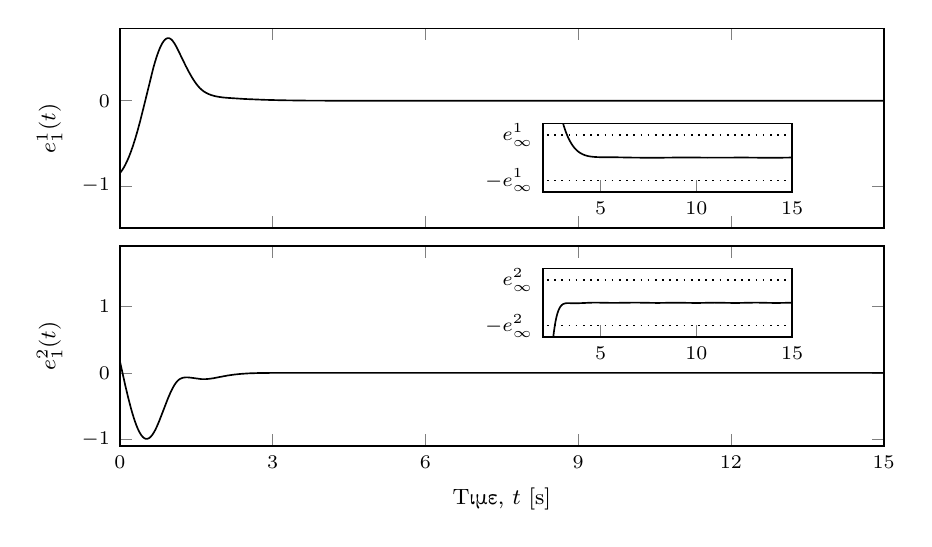
\begin{tikzpicture}

\begin{axis}[%
width=\figurewidth,
height=0.465\figureheight,
at={(0\figurewidth,0.507\figureheight)},
scale only axis,
xmin=0,
xmax=15,
xtick={0,3,6,9,12,15},
xticklabels={\empty},
ymin=-1.5,
ymax=0.85,
ylabel style={font=\color{white!15!black}},
ylabel={$e_1^1(t)$},
axis background/.style={fill=white},
xlabel style={font=\footnotesize},ylabel style={font=\footnotesize},ticklabel style={font=\scriptsize},x tick label style={font=\scriptsize},y tick label style={font=\scriptsize},legend style={font=\scriptsize}
]
\addplot [color=black, forget plot]
  table[row sep=crcr]{%
0	-0.8507\\
0.0258893802924707	-0.83133801279727\\
0.0520778695758413	-0.808720731138516\\
0.0782663588592101	-0.783054379696107\\
0.104454848142579	-0.754347389463051\\
0.142041020175668	-0.707869292654339\\
0.179627192208757	-0.65524831563391\\
0.217213364241847	-0.59660849124977\\
0.255781988061594	-0.530355956384216\\
0.307444035131487	-0.432382995355201\\
0.349531300938498	-0.345240385108625\\
0.401819323285832	-0.228718737784833\\
0.464511975263539	-0.0790741154592336\\
0.655562682377669	0.386104001853798\\
0.694107409816993	0.466432839358843\\
0.727758652616339	0.529588911624179\\
0.76015588918292	0.58366189501357\\
0.789192926360474	0.62602908060013\\
0.814834428068346	0.658232871919166\\
0.838181192055682	0.683026304826184\\
0.859585369723888	0.701797047838037\\
0.882324815332606	0.717456338439804\\
0.899865893493281	0.726455067379609\\
0.920492649332115	0.733552371980974\\
0.941526145210046	0.73688063022909\\
0.960652569590914	0.73647659783156\\
0.978418718184152	0.733192660604947\\
1.00131218604304	0.724900487538706\\
1.02118160068197	0.714124503891458\\
1.04560956574671	0.696658313812959\\
1.07067249854314	0.674557817427647\\
1.10046320354967	0.643937500050072\\
1.1398422252138	0.598388317323455\\
1.21002694114195	0.511121112077211\\
1.29594209992101	0.405859939978473\\
1.35555585539707	0.337631970293339\\
1.41137717336915	0.278583202265185\\
1.45779119140665	0.23406421074862\\
1.49895909700305	0.199041961247774\\
1.53573824484431	0.171555461684036\\
1.57166116690962	0.148195431116783\\
1.60766419521011	0.128170202634395\\
1.64767246403025	0.109688052807671\\
1.69093626872893	0.0936342325015449\\
1.73769947971462	0.0798448550036266\\
1.7930125475609	0.0670181622550636\\
1.85545415655264	0.0561008216627492\\
1.92607148418924	0.0473342747610666\\
2.0188781175014	0.0391341335971891\\
2.11343112761492	0.0341943682472738\\
2.44858550135605	0.0208810366400876\\
2.83386994173132	0.0112180352447968\\
3.17241050662611	0.00582707212705458\\
3.61450539588635	0.00225806051783373\\
4.27621380766376	0.000412033226917075\\
6.01231356884686	5.92150261677915e-05\\
15	1.79372239248465e-05\\
};
\end{axis}

\begin{axis}[%
width=0.326\figurewidth,
height=0.159\figureheight,
at={(0.554\figurewidth,0.592\figureheight)},
scale only axis,
xmin=2,
xmax=15,
ytick={-0.005, 0.005},
xtick pos = bottom,
scaled y ticks = false,
ytick style={draw=none},
yticklabels={$-e_\infty^1$, $e_\infty^1$},
ymin=-0.0075,
ymax=0.0075,
axis background/.style={fill=white},
xlabel style={font=\footnotesize},ylabel style={font=\footnotesize},ticklabel style={font=\scriptsize},x tick label style={font=\scriptsize},y tick label style={font=\scriptsize},legend style={font=\scriptsize}
]
\addplot [color=black, forget plot]
  table[row sep=crcr]{%
3.04439448491035	0.00750919839340547\\
3.07429156077556	0.00708408880186084\\
3.10505224575437	0.00666744386960794\\
3.13723029650782	0.00625362768111515\\
3.16941468957564	0.00586232290233113\\
3.19984199370212	0.00551386985769753\\
3.23012617782407	0.00518778257292141\\
3.26313456376402	0.0048528478540657\\
3.29846175526377	0.00451476759324798\\
3.33616771663029	0.00417541431160728\\
3.37199140270746	0.00387267995468754\\
3.41149925167859	0.00356016385214808\\
3.45235714423201	0.00325933337198414\\
3.49369107497387	0.00297611106672058\\
3.53784161434843	0.00269471516072883\\
3.57833077426327	0.00245594186883835\\
3.61984681747332	0.00223004133241211\\
3.66747944986135	0.00199324246176147\\
3.71416573865901	0.00178275120535432\\
3.76271548101365	0.00158484722975594\\
3.81227934708108	0.00140330595775495\\
3.86675371124866	0.00122583898623851\\
3.92053525221204	0.00107121287373602\\
3.98117780083114	0.000918180968188409\\
4.04924667779683	0.000767915733137059\\
4.11742405323052	0.000638856356625084\\
4.18786138952567	0.000526521327552487\\
4.26431240998093	0.000425896979786344\\
4.34555994922191	0.000340011442927945\\
4.42364639484049	0.000277464804989691\\
4.53401500963362	0.000211083716621374\\
4.65107257161698	0.000160265564915107\\
4.79381716762074	0.000118954111403724\\
4.99649460942128	8.3499696717837e-05\\
5.1221852159191	7.7531649084861e-05\\
5.87419257741304	6.61634617191709e-05\\
6.49290862764376	1.59893477178485e-05\\
6.77124994303091	-4.58055381535871e-06\\
7.62745779151404	-3.0073444133194e-05\\
8.03038859415041	-2.77836643984841e-05\\
9.21827738551151	2.93408876235191e-05\\
9.97219220620731	1.94208361481429e-05\\
10.606419102346	-1.31913678060869e-05\\
10.8431973603513	-4.7069586326387e-06\\
11.3344103177505	1.01377186823015e-06\\
11.7614579931151	2.07287252251831e-07\\
12.2444392946398	1.54948503858776e-05\\
12.5346151286188	1.49092501580128e-05\\
13.2827998984117	-1.73059794565944e-05\\
14.0946364478967	-3.40743143159017e-05\\
14.3831878219361	-2.33107878582217e-05\\
15	1.79372239248465e-05\\
};
\addplot [color=black, dotted, forget plot]
  table[row sep=crcr]{%
0.699999999999999	0.00500000000000078\\
15	0.00500000000000078\\
};
\addplot [color=black, dotted, forget plot]
  table[row sep=crcr]{%
0.699999999999999	-0.00500000000000078\\
15	-0.00500000000000078\\
};
\end{axis}

\begin{axis}[%
width=\figurewidth,
height=0.465\figureheight,
at={(0\figurewidth,0\figureheight)},
scale only axis,
xmin=0,
xmax=15,
xtick={ 0,  3,  6,  9, 12, 15},
xlabel style={font=\color{white!15!black}},
xlabel={Time, $t$ [\si{\second}]},
ymin=-1.1,
ymax=1.9,
ylabel style={font=\color{white!15!black}},
ylabel={$e_1^2(t)$},
axis background/.style={fill=white},
xlabel style={font=\footnotesize},ylabel style={font=\footnotesize},ticklabel style={font=\scriptsize},x tick label style={font=\scriptsize},y tick label style={font=\scriptsize},legend style={font=\scriptsize}
]
\addplot [color=black, forget plot]
  table[row sep=crcr]{%
0	0.172000000000001\\
0.104454848142579	-0.187252911238449\\
0.160834106192212	-0.368327356852539\\
0.217213364241847	-0.533973754078618\\
0.255781988061594	-0.635992361160556\\
0.291500780498144	-0.720897312092333\\
0.323387289764831	-0.788085092192917\\
0.349531300938498	-0.836652846604647\\
0.375675312112165	-0.87901536112247\\
0.401819323285832	-0.91490581436325\\
0.429813286422668	-0.945906968233295\\
0.454288642188862	-0.966550069983358\\
0.478151286312224	-0.980769380252468\\
0.500152107828706	-0.988665810478674\\
0.519597716701773	-0.991476350000196\\
0.54071246563328	-0.990129227370556\\
0.561959403119758	-0.98423112170755\\
0.583925253852689	-0.973504935474516\\
0.608000073110238	-0.956614512700005\\
0.631696366012312	-0.935023877946032\\
0.655562682377669	-0.908571713179844\\
0.687377161257125	-0.866462109466715\\
0.721028404056471	-0.814195043229923\\
0.763357164902455	-0.738972472609115\\
0.818169680066537	-0.631432019717383\\
0.941526145210046	-0.386687078662339\\
0.990262817246311	-0.29990719559618\\
1.03115913906562	-0.235232817423915\\
1.06616478659993	-0.187502468257922\\
1.09754574273095	-0.15172436171806\\
1.12600009952073	-0.125420337137832\\
1.15362428088711	-0.105479473964987\\
1.18153979556245	-0.0905658799304394\\
1.21111507284635	-0.0797236327974762\\
1.24433679598266	-0.0722775125442059\\
1.28392845049045	-0.0683045404389091\\
1.33355229857663	-0.0680324168688813\\
1.38895793137309	-0.072153924309351\\
1.60766419521011	-0.0946720200821005\\
1.67625091921728	-0.0945079056602793\\
1.74980545616616	-0.0900128304081935\\
1.83803649030618	-0.0804157852576459\\
1.95046566716839	-0.0635041314983962\\
2.11343112761492	-0.0401463651577973\\
2.25114320846735	-0.0252189310757505\\
2.38088406541299	-0.015053618439115\\
2.53459676957116	-0.00744342179267221\\
2.71978592836983	-0.00277128167257423\\
2.99815923011619	-0.000413995365041941\\
3.71416573865901	-9.62793370682391e-05\\
15	2.9791696698922e-05\\
};
\end{axis}

\begin{axis}[%
width=0.326\figurewidth,
height=0.159\figureheight,
at={(0.554\figurewidth,0.254\figureheight)},
scale only axis,
xmin=2,
xmax=15,
ymin=-0.0075,
ymax=0.0075,
ytick={-0.005, 0.005},
xtick pos = bottom,
scaled y ticks = false,
ytick style={draw=none},
yticklabels={$-e_\infty^2$, $e_\infty^2$},
axis background/.style={fill=white},
xlabel style={font=\footnotesize},ylabel style={font=\footnotesize},ticklabel style={font=\scriptsize},x tick label style={font=\scriptsize},y tick label style={font=\scriptsize},legend style={font=\scriptsize}
]
\addplot [color=black, forget plot]
  table[row sep=crcr]{%
2.53202725925877	-0.00753810391968202\\
2.54441718830964	-0.00709064573143436\\
2.55751107996095	-0.00664209776718572\\
2.56845119340846	-0.00628576410402637\\
2.57939130685597	-0.00594557371200821\\
2.59128528515524	-0.00559335103991465\\
2.60365619588038	-0.00524571422995024\\
2.61841572686722	-0.00485479481259254\\
2.63144024120738	-0.00453036299839304\\
2.64446475554755	-0.00422424946404476\\
2.65748926988771	-0.00393559037934033\\
2.67337602996843	-0.00360591815898204\\
2.68926279004915	-0.00329953324559717\\
2.70717215255628	-0.002980358793641\\
2.7260928162766	-0.00267139256819071\\
2.74044531343032	-0.0024551531337913\\
2.75653653192422	-0.00223018865218272\\
2.77661841616077	-0.00197372956960784\\
2.79670030039732	-0.00174235095066777\\
2.81900208519772	-0.00151240231403094\\
2.84130386999812	-0.00130833315073176\\
2.86360565479853	-0.00112758938079693\\
2.88590743959893	-0.000967764555275252\\
2.9139421069352	-0.000793198628056047\\
2.94083174604694	-0.000650148597198807\\
2.96817750450673	-0.000526444265696924\\
2.99596698807438	-0.000421425967283895\\
3.02376479706121	-0.000336116808156817\\
3.05506189491753	-0.000261507469046407\\
3.0910037037012	-0.000197720690064074\\
3.13293976778686	-0.0001437162102782\\
3.18459714832576	-9.86656767238969e-05\\
3.23841421982265	-7.27338175643411e-05\\
3.29846175526377	-6.53321374670668e-05\\
3.42506027556172	-7.69042459758396e-05\\
3.67438941804718	-9.71765702608707e-05\\
3.85486616127645	-8.51478570851327e-05\\
4.07453167992071	-4.89474429059555e-05\\
4.45344339553417	2.59041000543192e-05\\
4.65107257161698	4.4176914656191e-05\\
4.86396204181763	4.09035304649308e-05\\
5.39095056799544	-1.70668403853824e-08\\
5.65376271348305	-1.14537612656562e-05\\
5.96523906962545	-1.23042645050475e-06\\
6.77917617821224	4.69045481548136e-05\\
7.07818409564845	3.34476074108636e-05\\
7.97144180661933	-2.97555606376676e-05\\
8.2455159537499	-1.17983547909262e-05\\
8.81354916424361	3.36086349399523e-05\\
9.0691834082261	2.88787351951925e-05\\
9.45009317126906	-1.12713634869976e-06\\
9.89770414005185	-3.03738705742518e-05\\
10.1954609508851	-2.42489815871494e-05\\
10.5020726407525	2.24064534037893e-06\\
10.9476312348432	3.46137031588256e-05\\
11.2147317834358	2.80434216666237e-05\\
11.5353612525667	-2.62241844062316e-06\\
11.9519247861094	-3.1928184775154e-05\\
12.2351203692658	-2.39865563411712e-05\\
12.6046914339117	9.95124204372644e-06\\
13.0085905032293	3.85584735305144e-05\\
13.2954628893819	3.38431483868362e-05\\
13.6119932160703	5.54552234177663e-06\\
14.0634517889374	-3.07184657160064e-05\\
14.3279618909009	-2.73753360069406e-05\\
14.6063547700303	-3.75265192076313e-06\\
15	2.9791696698922e-05\\
};
\addplot [color=black, dotted, forget plot]
  table[row sep=crcr]{%
0.699999999999999	0.00500000000000078\\
15	0.00500000000000078\\
};
\addplot [color=black, dotted, forget plot]
  table[row sep=crcr]{%
0.699999999999999	-0.00500000000000078\\
15	-0.00500000000000078\\
};
\end{axis}
\end{tikzpicture}%
%      \begin{minipage}[t]{0.50\textwidth}
%          \selectlanguage{english}
%          \begin{center}
%              % This file was created by matlab2tikz.
%
\tikzstyle{every node}=[font=\footnotesize]
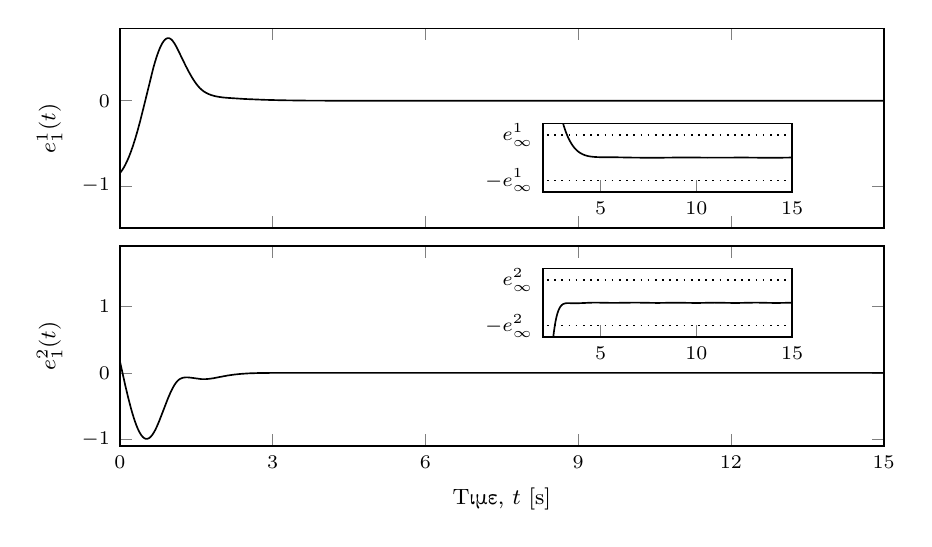
\begin{tikzpicture}

\begin{axis}[%
width=\figurewidth,
height=0.465\figureheight,
at={(0\figurewidth,0.507\figureheight)},
scale only axis,
xmin=0,
xmax=15,
xtick={0,3,6,9,12,15},
xticklabels={\empty},
ymin=-1.5,
ymax=0.85,
ylabel style={font=\color{white!15!black}},
ylabel={$e_1^1(t)$},
axis background/.style={fill=white},
xlabel style={font=\footnotesize},ylabel style={font=\footnotesize},ticklabel style={font=\scriptsize},x tick label style={font=\scriptsize},y tick label style={font=\scriptsize},legend style={font=\scriptsize}
]
\addplot [color=black, forget plot]
  table[row sep=crcr]{%
0	-0.8507\\
0.0258893802924707	-0.83133801279727\\
0.0520778695758413	-0.808720731138516\\
0.0782663588592101	-0.783054379696107\\
0.104454848142579	-0.754347389463051\\
0.142041020175668	-0.707869292654339\\
0.179627192208757	-0.65524831563391\\
0.217213364241847	-0.59660849124977\\
0.255781988061594	-0.530355956384216\\
0.307444035131487	-0.432382995355201\\
0.349531300938498	-0.345240385108625\\
0.401819323285832	-0.228718737784833\\
0.464511975263539	-0.0790741154592336\\
0.655562682377669	0.386104001853798\\
0.694107409816993	0.466432839358843\\
0.727758652616339	0.529588911624179\\
0.76015588918292	0.58366189501357\\
0.789192926360474	0.62602908060013\\
0.814834428068346	0.658232871919166\\
0.838181192055682	0.683026304826184\\
0.859585369723888	0.701797047838037\\
0.882324815332606	0.717456338439804\\
0.899865893493281	0.726455067379609\\
0.920492649332115	0.733552371980974\\
0.941526145210046	0.73688063022909\\
0.960652569590914	0.73647659783156\\
0.978418718184152	0.733192660604947\\
1.00131218604304	0.724900487538706\\
1.02118160068197	0.714124503891458\\
1.04560956574671	0.696658313812959\\
1.07067249854314	0.674557817427647\\
1.10046320354967	0.643937500050072\\
1.1398422252138	0.598388317323455\\
1.21002694114195	0.511121112077211\\
1.29594209992101	0.405859939978473\\
1.35555585539707	0.337631970293339\\
1.41137717336915	0.278583202265185\\
1.45779119140665	0.23406421074862\\
1.49895909700305	0.199041961247774\\
1.53573824484431	0.171555461684036\\
1.57166116690962	0.148195431116783\\
1.60766419521011	0.128170202634395\\
1.64767246403025	0.109688052807671\\
1.69093626872893	0.0936342325015449\\
1.73769947971462	0.0798448550036266\\
1.7930125475609	0.0670181622550636\\
1.85545415655264	0.0561008216627492\\
1.92607148418924	0.0473342747610666\\
2.0188781175014	0.0391341335971891\\
2.11343112761492	0.0341943682472738\\
2.44858550135605	0.0208810366400876\\
2.83386994173132	0.0112180352447968\\
3.17241050662611	0.00582707212705458\\
3.61450539588635	0.00225806051783373\\
4.27621380766376	0.000412033226917075\\
6.01231356884686	5.92150261677915e-05\\
15	1.79372239248465e-05\\
};
\end{axis}

\begin{axis}[%
width=0.326\figurewidth,
height=0.159\figureheight,
at={(0.554\figurewidth,0.592\figureheight)},
scale only axis,
xmin=2,
xmax=15,
ytick={-0.005, 0.005},
xtick pos = bottom,
scaled y ticks = false,
ytick style={draw=none},
yticklabels={$-e_\infty^1$, $e_\infty^1$},
ymin=-0.0075,
ymax=0.0075,
axis background/.style={fill=white},
xlabel style={font=\footnotesize},ylabel style={font=\footnotesize},ticklabel style={font=\scriptsize},x tick label style={font=\scriptsize},y tick label style={font=\scriptsize},legend style={font=\scriptsize}
]
\addplot [color=black, forget plot]
  table[row sep=crcr]{%
3.04439448491035	0.00750919839340547\\
3.07429156077556	0.00708408880186084\\
3.10505224575437	0.00666744386960794\\
3.13723029650782	0.00625362768111515\\
3.16941468957564	0.00586232290233113\\
3.19984199370212	0.00551386985769753\\
3.23012617782407	0.00518778257292141\\
3.26313456376402	0.0048528478540657\\
3.29846175526377	0.00451476759324798\\
3.33616771663029	0.00417541431160728\\
3.37199140270746	0.00387267995468754\\
3.41149925167859	0.00356016385214808\\
3.45235714423201	0.00325933337198414\\
3.49369107497387	0.00297611106672058\\
3.53784161434843	0.00269471516072883\\
3.57833077426327	0.00245594186883835\\
3.61984681747332	0.00223004133241211\\
3.66747944986135	0.00199324246176147\\
3.71416573865901	0.00178275120535432\\
3.76271548101365	0.00158484722975594\\
3.81227934708108	0.00140330595775495\\
3.86675371124866	0.00122583898623851\\
3.92053525221204	0.00107121287373602\\
3.98117780083114	0.000918180968188409\\
4.04924667779683	0.000767915733137059\\
4.11742405323052	0.000638856356625084\\
4.18786138952567	0.000526521327552487\\
4.26431240998093	0.000425896979786344\\
4.34555994922191	0.000340011442927945\\
4.42364639484049	0.000277464804989691\\
4.53401500963362	0.000211083716621374\\
4.65107257161698	0.000160265564915107\\
4.79381716762074	0.000118954111403724\\
4.99649460942128	8.3499696717837e-05\\
5.1221852159191	7.7531649084861e-05\\
5.87419257741304	6.61634617191709e-05\\
6.49290862764376	1.59893477178485e-05\\
6.77124994303091	-4.58055381535871e-06\\
7.62745779151404	-3.0073444133194e-05\\
8.03038859415041	-2.77836643984841e-05\\
9.21827738551151	2.93408876235191e-05\\
9.97219220620731	1.94208361481429e-05\\
10.606419102346	-1.31913678060869e-05\\
10.8431973603513	-4.7069586326387e-06\\
11.3344103177505	1.01377186823015e-06\\
11.7614579931151	2.07287252251831e-07\\
12.2444392946398	1.54948503858776e-05\\
12.5346151286188	1.49092501580128e-05\\
13.2827998984117	-1.73059794565944e-05\\
14.0946364478967	-3.40743143159017e-05\\
14.3831878219361	-2.33107878582217e-05\\
15	1.79372239248465e-05\\
};
\addplot [color=black, dotted, forget plot]
  table[row sep=crcr]{%
0.699999999999999	0.00500000000000078\\
15	0.00500000000000078\\
};
\addplot [color=black, dotted, forget plot]
  table[row sep=crcr]{%
0.699999999999999	-0.00500000000000078\\
15	-0.00500000000000078\\
};
\end{axis}

\begin{axis}[%
width=\figurewidth,
height=0.465\figureheight,
at={(0\figurewidth,0\figureheight)},
scale only axis,
xmin=0,
xmax=15,
xtick={ 0,  3,  6,  9, 12, 15},
xlabel style={font=\color{white!15!black}},
xlabel={Time, $t$ [\si{\second}]},
ymin=-1.1,
ymax=1.9,
ylabel style={font=\color{white!15!black}},
ylabel={$e_1^2(t)$},
axis background/.style={fill=white},
xlabel style={font=\footnotesize},ylabel style={font=\footnotesize},ticklabel style={font=\scriptsize},x tick label style={font=\scriptsize},y tick label style={font=\scriptsize},legend style={font=\scriptsize}
]
\addplot [color=black, forget plot]
  table[row sep=crcr]{%
0	0.172000000000001\\
0.104454848142579	-0.187252911238449\\
0.160834106192212	-0.368327356852539\\
0.217213364241847	-0.533973754078618\\
0.255781988061594	-0.635992361160556\\
0.291500780498144	-0.720897312092333\\
0.323387289764831	-0.788085092192917\\
0.349531300938498	-0.836652846604647\\
0.375675312112165	-0.87901536112247\\
0.401819323285832	-0.91490581436325\\
0.429813286422668	-0.945906968233295\\
0.454288642188862	-0.966550069983358\\
0.478151286312224	-0.980769380252468\\
0.500152107828706	-0.988665810478674\\
0.519597716701773	-0.991476350000196\\
0.54071246563328	-0.990129227370556\\
0.561959403119758	-0.98423112170755\\
0.583925253852689	-0.973504935474516\\
0.608000073110238	-0.956614512700005\\
0.631696366012312	-0.935023877946032\\
0.655562682377669	-0.908571713179844\\
0.687377161257125	-0.866462109466715\\
0.721028404056471	-0.814195043229923\\
0.763357164902455	-0.738972472609115\\
0.818169680066537	-0.631432019717383\\
0.941526145210046	-0.386687078662339\\
0.990262817246311	-0.29990719559618\\
1.03115913906562	-0.235232817423915\\
1.06616478659993	-0.187502468257922\\
1.09754574273095	-0.15172436171806\\
1.12600009952073	-0.125420337137832\\
1.15362428088711	-0.105479473964987\\
1.18153979556245	-0.0905658799304394\\
1.21111507284635	-0.0797236327974762\\
1.24433679598266	-0.0722775125442059\\
1.28392845049045	-0.0683045404389091\\
1.33355229857663	-0.0680324168688813\\
1.38895793137309	-0.072153924309351\\
1.60766419521011	-0.0946720200821005\\
1.67625091921728	-0.0945079056602793\\
1.74980545616616	-0.0900128304081935\\
1.83803649030618	-0.0804157852576459\\
1.95046566716839	-0.0635041314983962\\
2.11343112761492	-0.0401463651577973\\
2.25114320846735	-0.0252189310757505\\
2.38088406541299	-0.015053618439115\\
2.53459676957116	-0.00744342179267221\\
2.71978592836983	-0.00277128167257423\\
2.99815923011619	-0.000413995365041941\\
3.71416573865901	-9.62793370682391e-05\\
15	2.9791696698922e-05\\
};
\end{axis}

\begin{axis}[%
width=0.326\figurewidth,
height=0.159\figureheight,
at={(0.554\figurewidth,0.254\figureheight)},
scale only axis,
xmin=2,
xmax=15,
ymin=-0.0075,
ymax=0.0075,
ytick={-0.005, 0.005},
xtick pos = bottom,
scaled y ticks = false,
ytick style={draw=none},
yticklabels={$-e_\infty^2$, $e_\infty^2$},
axis background/.style={fill=white},
xlabel style={font=\footnotesize},ylabel style={font=\footnotesize},ticklabel style={font=\scriptsize},x tick label style={font=\scriptsize},y tick label style={font=\scriptsize},legend style={font=\scriptsize}
]
\addplot [color=black, forget plot]
  table[row sep=crcr]{%
2.53202725925877	-0.00753810391968202\\
2.54441718830964	-0.00709064573143436\\
2.55751107996095	-0.00664209776718572\\
2.56845119340846	-0.00628576410402637\\
2.57939130685597	-0.00594557371200821\\
2.59128528515524	-0.00559335103991465\\
2.60365619588038	-0.00524571422995024\\
2.61841572686722	-0.00485479481259254\\
2.63144024120738	-0.00453036299839304\\
2.64446475554755	-0.00422424946404476\\
2.65748926988771	-0.00393559037934033\\
2.67337602996843	-0.00360591815898204\\
2.68926279004915	-0.00329953324559717\\
2.70717215255628	-0.002980358793641\\
2.7260928162766	-0.00267139256819071\\
2.74044531343032	-0.0024551531337913\\
2.75653653192422	-0.00223018865218272\\
2.77661841616077	-0.00197372956960784\\
2.79670030039732	-0.00174235095066777\\
2.81900208519772	-0.00151240231403094\\
2.84130386999812	-0.00130833315073176\\
2.86360565479853	-0.00112758938079693\\
2.88590743959893	-0.000967764555275252\\
2.9139421069352	-0.000793198628056047\\
2.94083174604694	-0.000650148597198807\\
2.96817750450673	-0.000526444265696924\\
2.99596698807438	-0.000421425967283895\\
3.02376479706121	-0.000336116808156817\\
3.05506189491753	-0.000261507469046407\\
3.0910037037012	-0.000197720690064074\\
3.13293976778686	-0.0001437162102782\\
3.18459714832576	-9.86656767238969e-05\\
3.23841421982265	-7.27338175643411e-05\\
3.29846175526377	-6.53321374670668e-05\\
3.42506027556172	-7.69042459758396e-05\\
3.67438941804718	-9.71765702608707e-05\\
3.85486616127645	-8.51478570851327e-05\\
4.07453167992071	-4.89474429059555e-05\\
4.45344339553417	2.59041000543192e-05\\
4.65107257161698	4.4176914656191e-05\\
4.86396204181763	4.09035304649308e-05\\
5.39095056799544	-1.70668403853824e-08\\
5.65376271348305	-1.14537612656562e-05\\
5.96523906962545	-1.23042645050475e-06\\
6.77917617821224	4.69045481548136e-05\\
7.07818409564845	3.34476074108636e-05\\
7.97144180661933	-2.97555606376676e-05\\
8.2455159537499	-1.17983547909262e-05\\
8.81354916424361	3.36086349399523e-05\\
9.0691834082261	2.88787351951925e-05\\
9.45009317126906	-1.12713634869976e-06\\
9.89770414005185	-3.03738705742518e-05\\
10.1954609508851	-2.42489815871494e-05\\
10.5020726407525	2.24064534037893e-06\\
10.9476312348432	3.46137031588256e-05\\
11.2147317834358	2.80434216666237e-05\\
11.5353612525667	-2.62241844062316e-06\\
11.9519247861094	-3.1928184775154e-05\\
12.2351203692658	-2.39865563411712e-05\\
12.6046914339117	9.95124204372644e-06\\
13.0085905032293	3.85584735305144e-05\\
13.2954628893819	3.38431483868362e-05\\
13.6119932160703	5.54552234177663e-06\\
14.0634517889374	-3.07184657160064e-05\\
14.3279618909009	-2.73753360069406e-05\\
14.6063547700303	-3.75265192076313e-06\\
15	2.9791696698922e-05\\
};
\addplot [color=black, dotted, forget plot]
  table[row sep=crcr]{%
0.699999999999999	0.00500000000000078\\
15	0.00500000000000078\\
};
\addplot [color=black, dotted, forget plot]
  table[row sep=crcr]{%
0.699999999999999	-0.00500000000000078\\
15	-0.00500000000000078\\
};
\end{axis}
\end{tikzpicture}%
%          \end{center}
%          \selectlanguage{greek}
%      \end{minipage}%\
%      \hfill
%      \begin{minipage}[t]{0.48\textwidth}
%        Σφάλματα παρακολούθησης εξόδου
%      \end{minipage}

    \end{frame}
    
    \begin{frame}
        \frametitle{Ακαδημαϊκό παράδειγμα}
        \selectlanguage{english}
        % This file was created by matlab2tikz.
%
\tikzstyle{every node}=[font=\footnotesize]
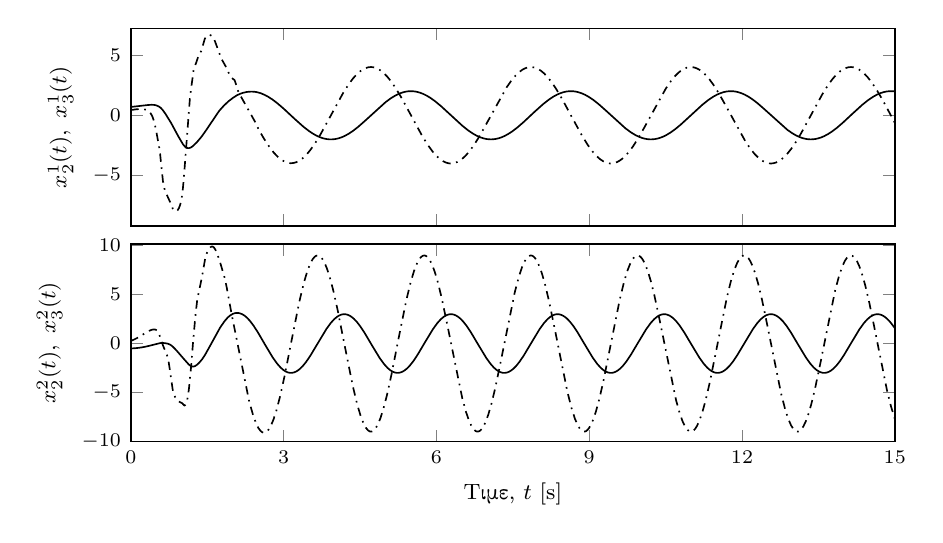
\begin{tikzpicture}

\begin{axis}[%
width=\figurewidth,
height=0.46\figureheight,
at={(0\figurewidth,0.501\figureheight)},
scale only axis,
xmin=0,
xmax=15,
xtick={0,3,6,9,12,15},
xticklabels={\empty},
ymin=-9.2,
ymax=7.2,
ylabel style={font=\color{white!15!black}},
ylabel={$x_2^1(t),\ x_3^1(t)$},
axis background/.style={fill=white},
xlabel style={font=\footnotesize},ylabel style={font=\footnotesize},ticklabel style={font=\scriptsize},x tick label style={font=\scriptsize},y tick label style={font=\scriptsize},legend style={font=\scriptsize}
]
\addplot [color=black, forget plot]
  table[row sep=crcr]{%
0	0.6904\\
0.160834106192212	0.767846843419173\\
0.336459295351665	0.852634311455237\\
0.401819323285832	0.868183473322999\\
0.442479769498089	0.863293055223536\\
0.478151286312224	0.841439437595922\\
0.512240604310017	0.797733493332169\\
0.549129795557976	0.721577073390209\\
0.585579808538007	0.611427278912021\\
0.622433164515732	0.442954820144706\\
0.68207474811055	0.08787824520026\\
0.789192926360474	-0.646193744898166\\
0.927368234611725	-1.72912082011149\\
1.02118160068197	-2.40445159764561\\
1.0620637387512	-2.60821415148699\\
1.09171082109352	-2.69356664333355\\
1.11703751383091	-2.72712633523306\\
1.13792410678431	-2.72533216888685\\
1.1619487330652	-2.69733738040062\\
1.18967473719271	-2.63799826780719\\
1.2278940147182	-2.51168079125101\\
1.29594209992101	-2.23010097734148\\
1.3869936803879	-1.77191521325112\\
1.45565213223369	-1.36585026991848\\
1.73366415423078	0.372033702747229\\
1.82803116969612	0.81303104632916\\
1.91646261019794	1.16554772792659\\
2.00612243030818	1.45383352824225\\
2.0831841700412	1.662896137184\\
2.14539162603574	1.78116208611714\\
2.20748000699365	1.86975246002527\\
2.26397855789261	1.92456463691164\\
2.31527046318562	1.95327541174526\\
2.36480386139433	1.96200648495015\\
2.41315883193432	1.95371966033903\\
2.45736497065977	1.93047537852226\\
2.50491292055109	1.88473873820531\\
2.56115778444345	1.80752717044875\\
2.6249279840373	1.69229656421927\\
2.69455837674273	1.53502815443069\\
2.77661841616077	1.31141116714705\\
2.87103958306533	1.01042245007605\\
2.99596698807438	0.558541387522814\\
3.21664848656974	-0.309824462718064\\
3.38718935515181	-0.951330300123539\\
3.49853868176765	-1.31612495855382\\
3.58779828795151	-1.56273848293392\\
3.66747944986135	-1.74134033808471\\
3.73237041046181	-1.85452318420671\\
3.79167583525255	-1.93083301940753\\
3.84407198183612	-1.97578316967533\\
3.89420331847394	-1.99857091003004\\
3.93782120655626	-2.00212560690995\\
3.98426417316842	-1.9892413240047\\
4.0327559033063	-1.95754922388561\\
4.08573518248294	-1.90192581715648\\
4.14396388490148	-1.81625592214062\\
4.20825929314959	-1.69318840800191\\
4.28209124518734	-1.51758893118498\\
4.36733769833703	-1.27408880103003\\
4.46775620496318	-0.940572497902608\\
4.59959594030997	-0.447778512702682\\
5.00182114727083	1.09402077472132\\
5.10367825757872	1.41022368035375\\
5.1887859695247	1.63005381314169\\
5.26368131753228	1.78473039381004\\
5.32844272340854	1.88636476831344\\
5.38596267534225	1.9501827089989\\
5.43850555024629	1.98600493332419\\
5.48627961382349	1.99952935652395\\
5.53044709836024	1.99576545507156\\
5.57745972129927	1.97466337875543\\
5.62562791472463	1.93496051175244\\
5.68075617538581	1.867538127188\\
5.74003870194739	1.76976170131093\\
5.80877895655185	1.62538701474815\\
5.88832765051244	1.42024267155857\\
5.97981500992158	1.14034409987316\\
6.09149874377907	0.748039831846826\\
6.25221066462731	0.123708189554277\\
6.51044508422304	-0.878170775469558\\
6.62531412752706	-1.26426886853279\\
6.71729512341257	-1.52640979491237\\
6.7943943599447	-1.70678147880713\\
6.86278600172654	-1.83299984130159\\
6.92285566155438	-1.91568144631938\\
6.97712997455088	-1.9666734162125\\
7.02698449949287	-1.99313763575174\\
7.07301514956759	-1.99997444317419\\
7.11956286218819	-1.98965417597241\\
7.16646822208493	-1.96182541257783\\
7.21746323883386	-1.91201085057538\\
7.27302158204332	-1.83514864706037\\
7.33501305187242	-1.72272634723957\\
7.40754740705084	-1.5577781003479\\
7.48844197253472	-1.33538015975923\\
7.58438416387551	-1.02690978891922\\
7.70678478597409	-0.580343832473615\\
7.92971961526699	0.301821762015937\\
8.0993358548506	0.942580056729113\\
8.20942301761797	1.30508206867581\\
8.30048730270663	1.55801306983371\\
8.3774409145081	1.73186294747138\\
8.44613736558862	1.85255209835942\\
8.50633887967683	1.92967315725241\\
8.55878154734728	1.97411503479648\\
8.60848922497025	1.99621822981013\\
8.65477159434245	1.99908463374929\\
8.70106984227337	1.98484650443692\\
8.74876906675137	1.95239358814121\\
8.80005396882393	1.89767847147582\\
8.85750806303247	1.81272078877123\\
8.9204580737753	1.69224140349973\\
8.9957773990789	1.51308581216718\\
9.08182390271961	1.26675024939768\\
9.18255049149944	0.931444428817683\\
9.31468767768609	0.436831551925261\\
9.7126805456825	-1.08904320564728\\
9.81566292972164	-1.40913304473385\\
9.90142178336015	-1.63071444521795\\
9.97639374112162	-1.78540475679225\\
10.0397945578047	-1.88506571885431\\
10.0960357560392	-1.94817470251843\\
10.1484503253794	-1.98483288735891\\
10.1954609508851	-1.99918192981336\\
10.2418026101387	-1.99604766780167\\
10.2886311803289	-1.97549087041961\\
10.3370137026239	-1.93605970731076\\
10.3908768519788	-1.87086453649511\\
10.4510133069447	-1.77248948602644\\
10.519433525253	-1.62951297190768\\
10.5973469142999	-1.42977421205037\\
10.6883782297119	-1.15287432308099\\
10.7981229465278	-0.76939634655611\\
10.9556045680085	-0.159688696966384\\
11.2244160408238	0.883747648898153\\
11.3400300337132	1.2713643875745\\
11.4329728924592	1.53479492543882\\
11.5121466443379	1.71781287630824\\
11.5817708214935	1.84336601912388\\
11.6428449082971	1.92418510505227\\
11.697359767872	1.97213661041383\\
11.7472545817268	1.99550734390741\\
11.793576962799	1.99941387056073\\
11.8389149944716	1.98662708550031\\
11.8839460890315	1.95777021747166\\
11.9372961490532	1.90307549644835\\
11.9924623446954	1.8237680221621\\
12.0528452326402	1.71158013526363\\
12.1247331965018	1.5456652398245\\
12.2074322180702	1.31560240712358\\
12.3053082244739	0.997467124014058\\
12.4297314740768	0.539771053791338\\
12.8906576084257	-1.20815115482565\\
12.9880942186321	-1.49390852826081\\
13.0665534204234	-1.68335783039504\\
13.1348604178839	-1.814752285093\\
13.1963430329301	-1.90416061339523\\
13.2533306704959	-1.9613849360134\\
13.3045532038899	-1.99113205185853\\
13.35124651637	-2.00004267152968\\
13.3980475353812	-1.99147204555479\\
13.4449210402166	-1.96541257643194\\
13.4960652839164	-1.91730249755538\\
13.5520880776453	-1.84163035639485\\
13.6119932160703	-1.73519654234964\\
13.6827612612501	-1.57756895115662\\
13.7630876965854	-1.36061107938006\\
13.857731208001	-1.06047609692372\\
13.9754017560096	-0.635854591688613\\
14.1669404872974	0.119041904398095\\
14.364478312728	0.878322340265607\\
14.4796032217388	1.26522639402433\\
14.572556635458	1.52974448593967\\
14.6527365378631	1.71586324829848\\
14.7225817278509	1.84222242577016\\
14.7830594488529	1.92271434859764\\
14.8366725983551	1.97060686955108\\
14.8861576387278	1.99473518307936\\
14.9336560005832	1.99953991350233\\
14.9792424339333	1.98721133075025\\
15	1.9761223720337\\
};
\addplot [color=black, dash dot, forget plot]
  table[row sep=crcr]{%
0	0.4773\\
0.000257073003341546	0.434700898760987\\
0.0913606035008936	0.490236779717721\\
0.160834106192212	0.515749341353903\\
0.198420278225301	0.518608386461324\\
0.23600645025839	0.509202808486048\\
0.2755575258648	0.479605246757304\\
0.307444035131487	0.433917162149335\\
0.336459295351665	0.36733057668769\\
0.362603306525331	0.277768879440091\\
0.388747317698998	0.147335013622666\\
0.422668912618699	-0.115569417579611\\
0.454288642188862	-0.507368656931853\\
0.489538504749916	-1.15688574627888\\
0.567043456591318	-2.96603362349448\\
0.592198027279284	-4.0533129457085\\
0.628608632180118	-5.48131809777736\\
0.655562682377669	-6.06080277614259\\
0.687377161257125	-6.44862770013244\\
0.779452332821029	-7.30111240291822\\
0.818169680066537	-7.73145489851482\\
0.847539419277211	-7.90250888025156\\
0.867165184926794	-7.95708408841704\\
0.882324815332606	-7.96758643563971\\
0.899865893493281	-7.94304723124412\\
0.920492649332115	-7.8596525225641\\
0.941526145210046	-7.70855475825282\\
0.966574619121994	-7.4282776929489\\
0.990262817246311	-7.02114148451309\\
1.01362535866852	-6.36578750622916\\
1.04045826513101	-5.09331794774401\\
1.15964505617575	1.52609670584198\\
1.22972350799145	3.73924382908951\\
1.33062612614889	4.9863936486768\\
1.39092218235828	5.40297514453027\\
1.41625456895759	5.84782504901482\\
1.44924953544752	6.34155862554804\\
1.47280345613076	6.521203922477\\
1.49895909700305	6.6233181475209\\
1.51910084123906	6.65819887859494\\
1.54128404604607	6.66362171141934\\
1.5595103185642	6.6451628740889\\
1.57773659108234	6.60596999053633\\
1.59971346855842	6.5266536673303\\
1.62693498940042	6.36113917774242\\
1.6528568326877	6.10556568063754\\
1.77336598485335	4.71084310136185\\
1.88674964027164	3.85867362907582\\
1.93119530424882	3.39073557915139\\
1.97110695298277	3.14174325393083\\
2.00357129286953	3.0153645750891\\
2.03298893155219	2.9281494907899\\
2.04510735011259	2.80294477648771\\
2.11172941851081	1.91285097519773\\
2.38088406541299	-0.11779241673695\\
2.43973074217723	-0.561593486961224\\
2.50725237591776	-1.17769278006701\\
2.61190346969714	-1.93927082428285\\
2.71978592836983	-2.63544011160402\\
2.80413422866412	-3.09714016195072\\
2.87847351133213	-3.43026707116618\\
2.94083174604694	-3.64654287545215\\
3.01644261869321	-3.85049620036074\\
3.06039559992111	-3.924784608168\\
3.09754427781956	-3.96270013884662\\
3.13293976778686	-3.97769906810656\\
3.16641887252516	-3.97260243989935\\
3.20464377110929	-3.94562591103654\\
3.24453224134868	-3.89744363095111\\
3.2842973680424	-3.82224984780691\\
3.33363232372085	-3.69360939394459\\
3.38718935515181	-3.5129580576966\\
3.45235714423201	-3.23945676887159\\
3.52486773577222	-2.87000440774204\\
3.61450539588635	-2.32962747276381\\
3.72023396259328	-1.59832528212733\\
3.86930320489183	-0.453436257800224\\
4.16496482400317	1.83667752888128\\
4.27621380766376	2.57530742706654\\
4.3678587481775	3.0912242876741\\
4.44058193422572	3.42515203015119\\
4.50006371953798	3.64665431201419\\
4.56224305016477	3.82240543087508\\
4.61181542144438	3.92060255099279\\
4.65107257161698	3.97110265578138\\
4.6873019488232	3.99600426338795\\
4.71487707332729	4.00090293401391\\
4.74245219783138	3.99363447186157\\
4.77669551102429	3.96771266002644\\
4.8109388242172	3.92319684712693\\
4.85393352910128	3.84131538155051\\
4.90494467572996	3.70745676436264\\
4.96342840803239	3.50673849789871\\
5.03097886525652	3.21673582118914\\
5.09972144853062	2.85854166376338\\
5.1887859695247	2.317407169233\\
5.2956416752367	1.57354818991171\\
5.44777835915058	0.400141062852116\\
5.71974175805279	-1.71808918966528\\
5.83442018326502	-2.49423766462701\\
5.92780166951846	-3.03104679286447\\
6.00688365892944	-3.40485653500071\\
6.07421802732694	-3.65589034171106\\
6.13253600736722	-3.81995723357433\\
6.1823790450646	-3.91931066603341\\
6.22554977541004	-3.97401373697032\\
6.26218182239927	-3.99663451836754\\
6.29546204232956	-3.99873253513354\\
6.32890690281243	-3.9831567764541\\
6.36550422401399	-3.94578724709186\\
6.40781733548697	-3.87631722438069\\
6.45580734975229	-3.76418003357179\\
6.50877419130584	-3.5995752570479\\
6.5690148665271	-3.36366918272871\\
6.63861544190974	-3.03091227976484\\
6.71729512341257	-2.58456253325857\\
6.81492288008386	-1.94324051217172\\
6.94238956623078	-0.998933982975442\\
7.37784795524564	2.31900029445415\\
7.47512668729794	2.90580167062383\\
7.55503122797633	3.30620204575883\\
7.62546309616175	3.5893769352444\\
7.68559335006242	3.77528650340305\\
7.73752999574501	3.89221377761995\\
7.77993310734368	3.95647258924388\\
7.81704064945095	3.9893434273524\\
7.85312839580836	4.00023622170617\\
7.88554045922697	3.99226477494192\\
7.92213597061812	3.96312146673372\\
7.96189728054924	3.90743945970819\\
8.00684254914657	3.81486347722659\\
8.05697162991938	3.67523976761159\\
8.11527888194212	3.46618242519853\\
8.18243983177916	3.16743322203568\\
8.26132322819375	2.74449407604484\\
8.35185814468628	2.1753630421511\\
8.46602346372577	1.35896342952564\\
8.64142464791375	-0.0163530617911629\\
8.8616542220396	-1.72046945493555\\
8.97445039558102	-2.48456789806562\\
9.0691834082261	-3.0304905851003\\
9.14849163946343	-3.40474854380414\\
9.21502512529542	-3.65280207091319\\
9.27487038243962	-3.82146627078202\\
9.32478185463932	-3.9203912329061\\
9.36737611074542	-3.97380508596714\\
9.40462583172781	-3.99683036050659\\
9.43913760357192	-3.99828113860491\\
9.47397459805372	-3.98034358684276\\
9.5105334759238	-3.9412495082009\\
9.55158632087355	-3.87229905519817\\
9.59921343371162	-3.75932621327511\\
9.65214921869934	-3.59373514264774\\
9.7126805456825	-3.35524519651683\\
9.78413935863699	-3.01104977566581\\
9.86327370109372	-2.55792820703912\\
9.96378913637868	-1.89228381813804\\
10.0918808913863	-0.937442456836958\\
10.5046988176444	2.22252636390274\\
10.6044665540546	2.83775471712392\\
10.6874558741978	3.26450229595915\\
10.760130536546	3.56450999036309\\
10.8200741449914	3.75595496550035\\
10.8726203860337	3.87953431066852\\
10.9145062389153	3.94743128642879\\
10.9476312348432	3.98153524082401\\
10.9795245675042	3.99786220020481\\
11.0115278454429	3.99789750819587\\
11.0446341300603	3.98070296724182\\
11.0810494347135	3.94164484314712\\
11.1234337060755	3.86988456362491\\
11.1688940272335	3.76203802823461\\
11.2244160408238	3.58825002560633\\
11.2866839895261	3.34077475085648\\
11.3592790138485	2.98738250021685\\
11.4413889570139	2.51279512813792\\
11.5399733137927	1.85445847920207\\
11.6700669500538	0.880292501092182\\
12.0673121895708	-2.167596086229\\
12.1691342204367	-2.80258037178262\\
12.2535042614264	-3.24225262681401\\
12.3233955441307	-3.5371841006927\\
12.3860476917459	-3.74289405779427\\
12.4401097186596	-3.87341158791619\\
12.485914804207	-3.94889872971661\\
12.5256294567497	-3.98720639092777\\
12.5616453779708	-3.9999267846264\\
12.5939358616187	-3.99389634988745\\
12.6286780877983	-3.96892547440375\\
12.6662811063252	-3.92038119128108\\
12.7105229763528	-3.83499585411025\\
12.7599985212251	-3.70405807167943\\
12.8173035283688	-3.50650827554906\\
12.88289028232	-3.22465668023351\\
12.9596951752153	-2.82470061687274\\
13.0447786281848	-2.30441052639829\\
13.1551521409428	-1.53265463127222\\
13.3106012205231	-0.329196059417267\\
13.5775830442034	1.74576196150089\\
13.6910498052818	2.51024201147672\\
13.7812767941931	3.02897811761862\\
13.857731208001	3.39148650534738\\
13.9254953172019	3.64675807129341\\
13.9835330898513	3.8127187337003\\
14.0319625209032	3.912010301532\\
14.0733916055381	3.9677606544789\\
14.1094527968281	3.99410533359527\\
14.1425568635615	4.00000315843962\\
14.1779648612476	3.98691514698826\\
14.209735006231	3.95816597395787\\
14.247828287649	3.90267639630985\\
14.2912995372693	3.81178981406091\\
14.3406996792043	3.67351793548224\\
14.3988152692318	3.46477638740297\\
14.4637916201263	3.17636899898661\\
14.5421981051197	2.75789499731093\\
14.6324168618496	2.19298930436092\\
14.7463155054467	1.38071225865706\\
14.9156096066809	0.0555962909193273\\
15	-0.616496481986548\\
};
\end{axis}

\begin{axis}[%
width=\figurewidth,
height=0.46\figureheight,
at={(0\figurewidth,0\figureheight)},
scale only axis,
xmin=0,
xmax=15,
xtick={ 0,  3,  6,  9, 12, 15},
xlabel style={font=\color{white!15!black}},
xlabel={Time, $t$ [\si{\second}]},
ymin=-10,
ymax=10.2,
ylabel style={font=\color{white!15!black}},
ylabel={$x_2^2(t),\ x_3^2(t)$},
axis background/.style={fill=white},
xlabel style={font=\footnotesize},ylabel style={font=\footnotesize},ticklabel style={font=\scriptsize},x tick label style={font=\scriptsize},y tick label style={font=\scriptsize},legend style={font=\scriptsize}
]
\addplot [color=black, forget plot]
  table[row sep=crcr]{%
0	-0.506500000000001\\
0.0782663588592101	-0.478317323830696\\
0.142041020175668	-0.444040202445198\\
0.217213364241847	-0.387899618512431\\
0.291500780498144	-0.314173905777521\\
0.375675312112165	-0.21010258124031\\
0.572928295644111	0.0462935224356738\\
0.608000073110238	0.0575851733864532\\
0.645334261078229	0.051110409145771\\
0.68207474811055	0.0289521051236115\\
0.721028404056471	-0.0137853007809436\\
0.75375333774385	-0.0731786228516391\\
0.784322629590751	-0.162305172096199\\
0.82484018406292	-0.33490473903076\\
0.892990308213669	-0.699319681965497\\
1.04560956574671	-1.61569871059687\\
1.13792410678431	-2.15500486606561\\
1.17672502181114	-2.3009539530319\\
1.20086420742117	-2.34466602545586\\
1.22107803596211	-2.35060578707029\\
1.24129519325883	-2.33507982097055\\
1.26385164784228	-2.28965282750898\\
1.29390482408732	-2.18434982476718\\
1.34029394788292	-1.9583559549838\\
1.39885252570949	-1.59906886044693\\
1.45351307306072	-1.16860720493168\\
1.54735947021878	-0.294631614211827\\
1.74980545616616	1.62011195215553\\
1.83303383000115	2.25282918397454\\
1.89960112338797	2.65766268465126\\
1.95046566716839	2.88067790367614\\
1.99735659053487	3.02475131227792\\
2.03460594727999	3.096800355311\\
2.06537432478759	3.12614160311658\\
2.09189009733685	3.12990241373217\\
2.11885013578146	3.11430256388753\\
2.15017016953609	3.07240780112183\\
2.18667494992151	2.9926055541433\\
2.22863576634768	2.85973224717829\\
2.27561187934731	2.65587840339546\\
2.33317495203115	2.33644966475122\\
2.40371537261646	1.85723171447329\\
2.49226104978239	1.14838731562078\\
2.63795249837747	-0.156020159759676\\
2.78331237757295	-1.41589777204551\\
2.87103958306533	-2.05757568886696\\
2.9427480585054	-2.4770079766969\\
2.99815923011619	-2.72316009072968\\
3.04439448491035	-2.87108712619687\\
3.08264393324835	-2.95158231440688\\
3.11631419765659	-2.99014009269184\\
3.14152082522878	-2.99899201779253\\
3.16941468957564	-2.98876849705087\\
3.1983194516169	-2.95608746083387\\
3.23219818832372	-2.8895182591114\\
3.27139052587231	-2.77532033800555\\
3.31676838748482	-2.5952303623563\\
3.37199140270746	-2.31156087436067\\
3.43951027990682	-1.87959743437311\\
3.52227979143264	-1.24727324320689\\
3.64311691130315	-0.198544195073467\\
3.83676655001389	1.47699481704202\\
3.92399244308088	2.10230479062031\\
3.99326808554389	2.4987102878113\\
4.04924667779683	2.74113896494976\\
4.09650248487276	2.8859950614346\\
4.13494320245137	2.96118592930525\\
4.16703690567631	2.99384339843021\\
4.19457333437222	2.99976286971698\\
4.22335645901508	2.98408476179688\\
4.25256089339284	2.9454580884348\\
4.28696682332568	2.87100380631168\\
4.32769198473756	2.74346441388005\\
4.37656421177025	2.53662852634651\\
4.4338218215692	2.2254529157124\\
4.50361437133676	1.7586326289141\\
4.58737645917555	1.09899503165457\\
4.73326048966335	-0.187727819506273\\
4.88401906725032	-1.47738190971465\\
4.97175953143377	-2.10590003543412\\
5.0392612256627	-2.49261043499549\\
5.09595366841899	-2.73921288464722\\
5.14242729593876	-2.88267595901972\\
5.18213276554592	-2.96100776154984\\
5.21408041829604	-2.99359895456341\\
5.24213339355111	-2.9995630323817\\
5.26906829852757	-2.98530930713804\\
5.29890379582019	-2.94678937936364\\
5.33363032141503	-2.8722818161606\\
5.37521105340627	-2.74219179995488\\
5.42382494328848	-2.53623054853497\\
5.47997608199921	-2.23164646181983\\
5.54808928526982	-1.77833948666765\\
5.63472235727578	-1.09768632780751\\
5.77428872897188	0.13230100933592\\
5.93089412499375	1.47485295752809\\
6.01794204466132	2.09936746930439\\
6.08659083184597	2.49325477174804\\
6.14233678303959	2.73622051514027\\
6.189624041457	2.88268909722779\\
6.22862913468234	2.96000158514886\\
6.26062784830456	2.99322086161394\\
6.28924078384934	2.99958514535215\\
6.31383013456971	2.98740526722432\\
6.34390239029779	2.95043884428752\\
6.37821306747174	2.8789867663235\\
6.41801602531492	2.75798600530496\\
6.46599755388382	2.56009429716103\\
6.52253166423154	2.25934551940422\\
6.58745371615955	1.83462109246233\\
6.67028997576202	1.19442039278347\\
6.79946708718886	0.0658329254933712\\
6.97480328156133	-1.44900142979144\\
7.06208482059526	-2.07964253780846\\
7.12978721001917	-2.47306261278345\\
7.18715968249856	-2.72740691756952\\
7.23549763572196	-2.87939349225524\\
7.27458171253557	-2.95818320109183\\
7.30632520931452	-2.9923045026337\\
7.33216761994939	-3.00006500369624\\
7.35883603430075	-2.98917939944601\\
7.38772425629318	-2.95581948971794\\
7.421304389135	-2.88918994846966\\
7.4607086783901	-2.77371529638909\\
7.50799115318942	-2.58422681468115\\
7.56305440499012	-2.29845032675903\\
7.62945248686633	-1.87146270096024\\
7.71376046471407	-1.22515176085793\\
7.83438284019342	-0.176297736094325\\
8.02327835627621	1.45904502915873\\
8.11077487270786	2.08929211421887\\
8.17848355332481	2.48067376385735\\
8.23682056171665	2.73656709634404\\
8.28441825221281	2.88369825597774\\
8.32342008841491	2.96059567576821\\
8.35490879869744	2.99316660528752\\
8.38189012163193	2.99984533870569\\
8.40858758139448	2.98711949858443\\
8.43974878771209	2.9480599545319\\
8.47365820260027	2.87633143638698\\
8.51369692628993	2.75343225766958\\
8.56137936506288	2.55547311314501\\
8.61730908054593	2.25710012945274\\
8.68578242783771	1.80650491787908\\
8.77225737068256	1.13162200458341\\
8.90784562975938	-0.0600048822243728\\
9.0691834082261	-1.44888049626077\\
9.15614701837203	-2.07746806362449\\
9.22609853469248	-2.48276960984751\\
9.28317230752725	-2.73342369000985\\
9.32982894311594	-2.87921055799106\\
9.36952074946143	-2.95897416900299\\
9.40163916033368	-2.99287133015381\\
9.43081149705507	-2.99959998144058\\
9.45766197676885	-2.98550127506994\\
9.48681315060893	-2.94828369561745\\
9.52149754515483	-2.87468582612999\\
9.56132737943311	-2.75187827142883\\
9.60918952095398	-2.55257699996436\\
9.66311377132781	-2.26533838891735\\
9.73145831431817	-1.81741768097199\\
9.81733666579937	-1.14925416190405\\
9.948435869302	0.000531457129255841\\
10.1168100793036	1.45224500141299\\
10.205408603898	2.0908184520515\\
10.2745016780359	2.48883828214012\\
10.3299911836987	2.73201731440518\\
10.3782346814129	2.88225925546792\\
10.4176183062926	2.96031287768232\\
10.448533376536	2.99269156584616\\
10.4758298389913	2.99989994748702\\
10.5020726407525	2.98787440169595\\
10.532211827259	2.9512410825101\\
10.5666869750716	2.87980672476067\\
10.606419102346	2.75937084527645\\
10.653824954993	2.56462108404423\\
10.7100542816532	2.26686745431036\\
10.7766709554339	1.83161684873046\\
10.8627373767201	1.1641847941385\\
10.9955262064736	0.000432490476548253\\
11.1628165215763	-1.44286775478713\\
11.2514885663473	-2.08361357122995\\
11.3201975617826	-2.4812927824143\\
11.3766113750589	-2.72988771080017\\
11.4236185523047	-2.87768753439281\\
11.4621399642332	-2.95630551233753\\
11.4945157013143	-2.99190145107587\\
11.5228024072944	-2.99992073868172\\
11.5481499810851	-2.98876434530767\\
11.5775634435056	-2.95417861645193\\
11.6113044367313	-2.88622889806914\\
11.6514197590037	-2.7670816417681\\
11.6989009899752	-2.57448358144615\\
11.7538225804863	-2.28695626170009\\
11.8198521698085	-1.86009350081194\\
11.9013971658429	-1.23459410105681\\
12.0241213980346	-0.167754762255942\\
12.2132313557945	1.46819753124038\\
12.2994027483357	2.08824985847157\\
12.3667742213195	2.47813720500621\\
12.4245598920985	2.7326737491314\\
12.4718013540572	2.88018218302737\\
12.5117757165612	2.95996633133532\\
12.5444749743478	2.99364029118529\\
12.5716045682373	2.99973394578291\\
12.5991049513295	2.9856435328016\\
12.6286780877983	2.9478364035525\\
12.6631397621261	2.87456415307879\\
12.7037310051318	2.74897053494055\\
12.7515040942506	2.54916307180805\\
12.8080361215347	2.24558014677043\\
12.8757298526591	1.79817610744416\\
12.962845952772	1.11661106755507\\
13.0991870600635	-0.0829520965232184\\
13.2586311182151	-1.45405131688242\\
13.3447853495899	-2.07648612790908\\
13.4116673278502	-2.46638529279912\\
13.4697582426852	-2.72519535757923\\
13.5178696874774	-2.87732252144628\\
13.5577984677322	-2.95822421852093\\
13.5881680631553	-2.9914036082655\\
13.6156317941676	-3.00004507800974\\
13.6439470017759	-2.98764658701914\\
13.6735003381331	-2.9517341331507\\
13.7082854458916	-2.87979601393289\\
13.7491216552467	-2.75544097706143\\
13.7971426724075	-2.5565340567517\\
13.8519455152498	-2.26510736915546\\
13.9193853753001	-1.82361389221771\\
14.0050401698603	-1.15829348778636\\
14.1364609576275	-0.00635666242559552\\
14.3061022358244	1.45620279922205\\
14.3939751038427	2.08938929096896\\
14.4602892475424	2.47366986043816\\
14.5183601972753	2.73046386844324\\
14.5656209907104	2.87872516360765\\
14.6054878559087	2.95895260600547\\
14.6377800440609	2.99297370380301\\
14.6661128007384	2.9997102588878\\
14.6933745852339	2.9857460841856\\
14.7241797628803	2.94596088036406\\
14.7584761658251	2.8721209308958\\
14.7992968871365	2.74473104919384\\
14.8472985886091	2.54249667883758\\
14.9035212304778	2.23906067818572\\
14.972808802444	1.77878559451548\\
15	1.57601991813808\\
};
\addplot [color=black, dash dot, forget plot]
  table[row sep=crcr]{%
0	0.332800000000001\\
0.00023329173099107	0.276929639032236\\
0.0520778695758413	0.387611924587375\\
0.123247934159123	0.573277819056928\\
0.217213364241847	0.869138939647756\\
0.336459295351665	1.24766466213595\\
0.388747317698998	1.37300775824506\\
0.429813286422668	1.43318031136819\\
0.454288642188862	1.44331792852287\\
0.475423424102488	1.42886654936744\\
0.497129983708378	1.3823342183682\\
0.51714534590452	1.29863335613914\\
0.538608133152106	1.14051898109767\\
0.560152981265576	0.861023844335071\\
0.631696366012312	-0.235226666768284\\
0.707567906936733	-1.17919424745491\\
0.736957086576151	-1.78072599330094\\
0.763357164902455	-2.67119898774317\\
0.818169680066537	-4.67119361770811\\
0.850550906888881	-5.27609419175476\\
0.882324815332606	-5.62663383240558\\
0.913617064052502	-5.83016424927328\\
0.941526145210046	-5.92993514747089\\
1.00606911665507	-6.09464996750794\\
1.03425884775409	-6.26992707776541\\
1.05076086636241	-6.33510803540701\\
1.0620637387512	-6.30746499465786\\
1.07558687458083	-6.19769254426659\\
1.09754574273095	-5.89244749878195\\
1.11918539155968	-5.40701182232508\\
1.14176034364329	-4.47915898920368\\
1.18394718243811	-2.20359734706757\\
1.21975053702575	0.178014676317472\\
1.26905936654659	3.01439260764407\\
1.30001665158838	4.39655598497105\\
1.33647847100438	5.36222298777643\\
1.39288643334346	6.75846995066683\\
1.45993025057962	8.76001635425303\\
1.4954547563723	9.30471437128968\\
1.53019244364256	9.6558105938171\\
1.5595103185642	9.83960402333456\\
1.58381201525505	9.91025482293362\\
1.59176274190673	9.91598717329347\\
1.59971346855842	9.91268328107672\\
1.61408779327354	9.88296838233174\\
1.63211935805788	9.80111011012949\\
1.65804120134516	9.59709499982893\\
1.69460760610684	9.1604782817254\\
1.75384078165001	8.24537791526\\
1.84572366111453	6.60958395199872\\
1.88048915892303	5.73103963950765\\
1.97939909271245	2.93026185603114\\
2.32191097922728	-5.92222834243228\\
2.3930213388433	-7.22045063308812\\
2.46045192871118	-8.18888630802093\\
2.50491292055109	-8.65112377964635\\
2.54441718830964	-8.92759581020308\\
2.57574460237347	-9.05938668204334\\
2.599532558972	-9.10735421021789\\
2.61841572686722	-9.1132276222293\\
2.63144024120738	-9.10064864202326\\
2.65097701271763	-9.05637480688992\\
2.67867161666201	-8.94170005461515\\
2.70717215255628	-8.76092464319223\\
2.74849092267727	-8.3883845222535\\
2.79670030039732	-7.79458964856671\\
2.85617172653173	-6.84218476431569\\
2.92802005038078	-5.41080195137806\\
3.01400189257054	-3.38597245052376\\
3.14581135394973	0.105686945078638\\
3.31048792995153	4.365316429413\\
3.39482396212082	6.19804050239996\\
3.46365492320134	7.40452842470565\\
3.51969184709306	8.15659864784167\\
3.56595249795947	8.60484491069831\\
3.60382255271242	8.84875395891505\\
3.63148186438824	8.95487518054287\\
3.65475195821807	8.9964224281624\\
3.67438941804718	8.99737625309077\\
3.68820935441883	8.97932250838934\\
3.70809751472475	8.92626524765613\\
3.73237041046181	8.81849183791178\\
3.76271548101365	8.61811982174109\\
3.80325997694811	8.23944464777109\\
3.84772469774724	7.68452643122597\\
3.90377953515288	6.79180031089911\\
3.97075183038416	5.4763714684394\\
4.05421607733039	3.5364882241754\\
4.18128047922125	0.202193767208204\\
4.3576796956921	-4.36762988673587\\
4.44283530511122	-6.21460911969929\\
4.51085096381265	-7.40501690008252\\
4.56726973196693	-8.1610905879445\\
4.61181542144438	-8.5940426417175\\
4.65107257161698	-8.8487220474591\\
4.67811024065517	-8.95297912750739\\
4.69649365699123	-8.99027052720928\\
4.71487707332729	-9.00022612175307\\
4.73326048966335	-8.98281598401842\\
4.7510130261296	-8.94007944327761\\
4.77669551102429	-8.83343817706724\\
4.8109388242172	-8.60988411742092\\
4.85393352910128	-8.20104881450333\\
4.89971327361005	-7.61619286558916\\
4.95811984568512	-6.66353396203444\\
5.02681149864275	-5.28400666143558\\
5.11398752883713	-3.22104078978473\\
5.25829433653699	0.601914022776429\\
5.40802733457071	4.44173112893458\\
5.49326421118516	6.27739982536279\\
5.55904312839434	7.42007621917096\\
5.61653347217348	8.18415021837684\\
5.66456009824416	8.63699918274729\\
5.70294831290958	8.87060113562095\\
5.73093738814826	8.96697371697454\\
5.75369067264609	8.99878337806153\\
5.76854035770855	8.9969452393091\\
5.78578547149854	8.97241108655634\\
5.80877895655185	8.90237555897171\\
5.83830972041909	8.75039281511738\\
5.87419257741304	8.47352323158438\\
5.91493674471379	8.04044880438696\\
5.96523906962545	7.34102721696554\\
6.02580125122199	6.27901386657095\\
6.09926125507794	4.71779041164364\\
6.1957891539982	2.33292822114993\\
6.50565066291395	-5.57082969265737\\
6.58007817630657	-6.99773351208139\\
6.64204122439602	-7.92323292205886\\
6.69127239320976	-8.46524252468219\\
6.73383605881401	-8.78559315964499\\
6.76728682544024	-8.93713547368481\\
6.78932163270055	-8.98788748766715\\
6.80453981443301	-9.00002484072801\\
6.82023321849056	-8.99289860360437\\
6.83616423371065	-8.9652813559087\\
6.85744062532864	-8.89648556390746\\
6.88841928460269	-8.73164893258636\\
6.92285566155438	-8.46006406992115\\
6.96656662010676	-7.98594450328225\\
7.01777746242016	-7.2567492436593\\
7.07818409564845	-6.17817366221283\\
7.15335639977667	-4.55831048935871\\
7.25368424439385	-2.05270721234798\\
7.53903964467682	5.27312010257745\\
7.61748431475258	6.82841594321695\\
7.68024742249619	7.805353076827\\
7.73158761298728	8.40046396218399\\
7.77499176950247	8.74884211388383\\
7.80547918895597	8.90522978726599\\
7.83438284019342	8.984766228892\\
7.85312839580836	9.0002766557115\\
7.87257563385952	8.98629520377738\\
7.88554045922697	8.95997980931423\\
7.90488170372183	8.8955504717511\\
7.93730325991586	8.72054811137741\\
7.97509406767664	8.41268831460849\\
8.01853819769341	7.92564968283751\\
8.06994204252618	7.17661651390469\\
8.13281926185052	6.03079536056129\\
8.20942301761797	4.3502616024898\\
8.31517501773489	1.67508107340997\\
8.57177063592527	-4.95188804222124\\
8.65346758158358	-6.62739521850228\\
8.71866715186711	-7.68445538860122\\
8.77225737068256	-8.33557760636481\\
8.81653396963943	-8.71176164474126\\
8.84921574501821	-8.89122216578099\\
8.87521201800345	-8.97304175079692\\
8.89627392980183	-8.99934312590848\\
8.91415185176734	-8.9934859428587\\
8.93307051779121	-8.95912384238296\\
8.95941882881737	-8.86323965888287\\
8.99044564820443	-8.67944031148719\\
9.02853698486844	-8.35126944739667\\
9.07591704312885	-7.79167228701044\\
9.13120229781972	-6.94096353606705\\
9.1974410361723	-5.67326495201268\\
9.27937876036311	-3.80275095353839\\
9.39566581754541	-0.784876823716287\\
9.59671941190103	4.43947273198157\\
9.68200161261622	6.27628857862493\\
9.75117234551509	7.47058149121334\\
9.80769704208739	8.2105409174458\\
9.85381828517011	8.64057661180212\\
9.8919136721387	8.87147364024354\\
9.92000999990167	8.96770688422194\\
9.93943342799175	8.99702953208426\\
9.95355362499422	8.99917579307164\\
9.97219220620731	8.9772882060296\\
9.99455898641705	8.91399151263562\\
10.0244071059012	8.76710586597961\\
10.0597337123594	8.50262539306021\\
10.1001906206921	8.08279233797069\\
10.151439382346	7.38124580116194\\
10.2103824304045	6.36020241341317\\
10.2827658714893	4.83890428536924\\
10.3766355263837	2.53966133029773\\
10.7046473111088	-5.78445847263562\\
10.7766709554339	-7.1282845418091\\
10.83346501921	-7.95684032786571\\
10.8825033953473	-8.48752035457959\\
10.9202323487811	-8.77144037043646\\
10.9556045680085	-8.93571493868908\\
10.9795245675042	-8.98989475227252\\
10.9955262064736	-9.00031563949329\\
11.0115278454429	-8.99000042268784\\
11.0275294844123	-8.95897303180315\\
11.0537379562236	-8.86361910679006\\
11.0810494347135	-8.70599744548879\\
11.1158973096395	-8.42026127724381\\
11.1628165215763	-7.89106173922812\\
11.2179598692318	-7.07057672339529\\
11.2826988801765	-5.86280138677216\\
11.3618212691633	-4.09260703511415\\
11.4722479145455	-1.2626539806323\\
11.7017675026097	4.68748569668853\\
11.7831202771719	6.40519401815803\\
11.8489577344793	7.5213888674213\\
11.9049383187293	8.24184126598706\\
11.9519247861094	8.66813202936525\\
11.9879396227898	8.8787908976163\\
12.0150759542234	8.96921079322717\\
12.0336960095698	8.996911433011\\
12.0528452326402	8.99612961517479\\
12.0721520151523	8.96529713399209\\
12.0963511430599	8.88421649370469\\
12.1247331965018	8.72953647846938\\
12.1610135376491	8.4399247867443\\
12.204714437828	7.95887081063713\\
12.2566200904434	7.21075392041152\\
12.3174834560306	6.11281947764362\\
12.3933791111448	4.46408363196814\\
12.4950917263374	1.90999009105009\\
12.7701539437435	-5.16612083400744\\
12.8487168453282	-6.74419356955266\\
12.9110663063922	-7.73480318941605\\
12.962845952772	-8.35366537116763\\
13.00346643208	-8.69892327178972\\
13.0393349301252	-8.89663594095425\\
13.0665534204234	-8.97806494528797\\
13.0834063174391	-8.99851113141563\\
13.0991870600635	-8.99680867866686\\
13.1188175435196	-8.96655903714621\\
13.1399333486486	-8.89932152292483\\
13.170162502848	-8.74103145762322\\
13.2062424596294	-8.45822889161003\\
13.2503740746983	-7.9782064911768\\
13.3007503812298	-7.26016064614961\\
13.360178437698	-6.20153825900563\\
13.4327278617861	-4.64680449874322\\
13.5327136514328	-2.16186598159097\\
13.8260779061246	5.35706085785572\\
13.9038565473999	6.88416036294814\\
13.9652905990536	7.83020555280921\\
14.0165763416282	8.41781498975177\\
14.0577609408085	8.74619316796432\\
14.090387479425	8.91185050802072\\
14.1143915798053	8.97931643565339\\
14.1303650516936	8.99843233670676\\
14.1486527694955	8.99495217600947\\
14.1669404872974	8.96440561193079\\
14.1953840035281	8.86335238577984\\
14.224086008934	8.69600879208953\\
14.2622591081794	8.37389789293786\\
14.3061022358244	7.86894630525501\\
14.3591705437622	7.07698008231528\\
14.422098810719	5.90763110310414\\
14.500179008143	4.17021416535355\\
14.6100752046492	1.36324875592707\\
14.8447623230125	-4.71975676692518\\
14.9272694507019	-6.45340120418056\\
14.993188757414	-7.56006014319617\\
15	-7.65829028138281\\
};
\end{axis}
\end{tikzpicture}%
    \end{frame}
    
    \begin{frame}
        \frametitle{Ακαδημαϊκό παράδειγμα}
        \selectlanguage{english}
        % This file was created by matlab2tikz.
%
\tikzstyle{every node}=[font=\footnotesize]
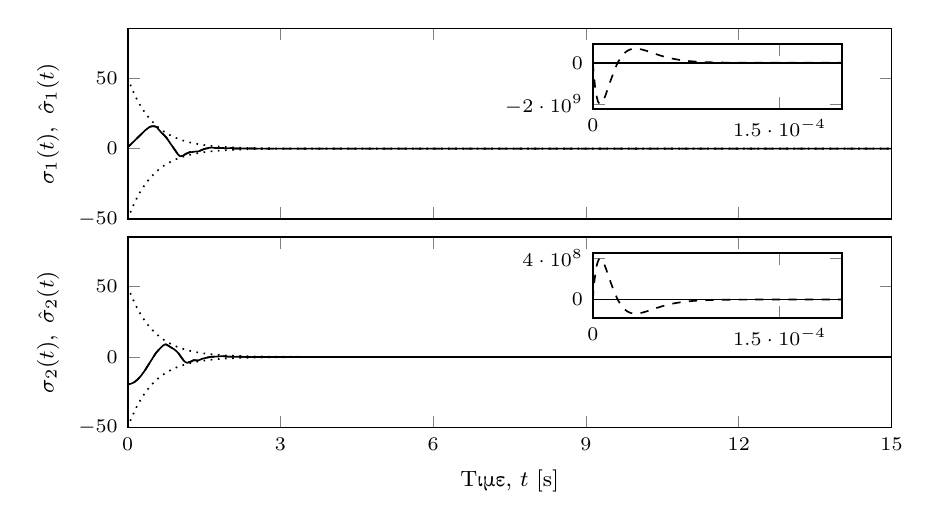
\begin{tikzpicture}

\begin{axis}[%
width=\figurewidth,
height=0.444\figureheight,
at={(0\figurewidth,0.485\figureheight)},
scale only axis,
unbounded coords=jump,
xmin=0,
xmax=15,
xtick={0,3,6,9,12,15},
xticklabels={\empty},
ymin=-50,
ymax=85,
ylabel style={font=\color{white!15!black}},
ylabel={$\sigma_1(t),\ \hat \sigma_1(t)$},
axis background/.style={fill=white},
xlabel style={font=\footnotesize},ylabel style={font=\footnotesize},ticklabel style={font=\scriptsize},x tick label style={font=\scriptsize},y tick label style={font=\scriptsize},legend style={font=\scriptsize}
]
\addplot [color=black, forget plot]
  table[row sep=crcr]{%
0	0.9634\\
0.000246628866978682	0.928955551848901\\
0.142041020175668	5.89232558769147\\
0.349531300938498	13.1464472957026\\
0.412267990909623	14.876030426447\\
0.450880864497304	15.5858301579675\\
0.475423424102488	15.8130286821387\\
0.489538504749916	15.8571277922097\\
0.500152107828706	15.8535819401211\\
0.514692975107268	15.8080742029274\\
0.536503800670932	15.6714846777525\\
0.555195892866781	15.4651500150099\\
0.571457085880914	15.1037627843252\\
0.592198027279284	14.2321848298383\\
0.648743734844709	11.7972393974103\\
0.769711739281581	7.31151965458073\\
0.878534907731153	1.46640435499472\\
0.984340767715231	-3.99529609945366\\
1.01740347967524	-5.12167984112393\\
1.03425884775409	-5.33590493245866\\
1.04045826513101	-5.34296507738832\\
1.04818521605456	-5.30316664095705\\
1.07312968656198	-5.01554213149768\\
1.10338066436838	-4.63463319374656\\
1.13216975149585	-3.86319263605152\\
1.15362428088711	-3.50337376499732\\
1.17552132837331	-3.21215369704484\\
1.21709553915303	-2.49211872477725\\
1.23155300126469	-2.44924991752823\\
1.24433679598266	-2.46239579719968\\
1.25719771566868	-2.48002862492911\\
1.26732346031182	-2.4485601695871\\
1.28779299658626	-2.28009276729484\\
1.31142994617537	-2.14123009237245\\
1.33062612614889	-2.09931812392744\\
1.37147529734574	-2.05282053152131\\
1.38502942940271	-1.98079658257961\\
1.40089011610514	-1.78779145782602\\
1.4884460751108	-0.433101139387684\\
1.55343489439149	0.187116686894349\\
1.60766419521011	0.589484694059504\\
1.63211935805788	0.690579449605034\\
1.64767246403025	0.706902691907279\\
1.66322557000262	0.680384357098575\\
1.68726493135101	0.576610157019827\\
1.72962882874693	0.392582655217353\\
1.75384078165001	0.346666336117345\\
1.77336598485335	0.338261260015619\\
1.79801520786593	0.353346888922724\\
1.86428452160354	0.417817997305287\\
1.87827375029721	0.384232627393022\\
1.93587343337058	0.181642535722665\\
1.95298453261194	0.183450389821878\\
1.97387099955933	0.214318985449639\\
1.99424923936755	0.279698506846502\\
2.02142925494005	0.431067800914803\\
2.03783997873559	0.491889995441012\\
2.04645179675305	0.461073173934116\\
2.06537432478759	0.278704829455856\\
2.08840114083922	0.121190656475788\\
2.10832600030258	0.0780880667744253\\
2.13507166138974	0.0619136092706665\\
2.18887827355335	0.0392744051560321\\
2.22228550890858	0.0231266280283542\\
2.34552829531026	0.0364970090586834\\
2.37760780217245	0.0641085754978601\\
2.42968488574057	0.125493743502636\\
2.44504359768452	0.101669594251881\\
2.47930799578244	0.0368661703506383\\
2.50959183128442	0.0203803906524573\\
2.56480448892596	0.0124254222201898\\
2.85617172653173	0.00344920030848073\\
2.9427480585054	0.0126031780778213\\
2.97791313687798	0.0105478372991001\\
3.04172763240856	0.00350394111224439\\
3.18706710250367	0.00569019289308059\\
3.26726254481816	0.00115155970243208\\
3.5618264058582	-0.000871770875086497\\
4.65107257161698	0.000420248434506831\\
12.4913968566613	-0.000652708727386653\\
13.3150515089598	-0.00059978804929095\\
13.9018539252874	-0.000442936020501605\\
15	0.00102549566699039\\
};
\addplot [color=black, dashed, forget plot]
  table[row sep=crcr]{%
0	0\\
7.105427357601e-14	-60\\
nan	nan\\
2.00029029926441e-05	-60.0000000074506\\
2.0002904022931e-05	60\\
nan	nan\\
0.000245787760697169	50.9032346138029\\
0.000372079771530309	0.933486489126018\\
0.0913606035008954	4.07912940398067\\
0.36260330652533	13.5454936175153\\
0.422668912618697	15.1033908420666\\
0.457696419880421	15.6689687147028\\
0.478151286312226	15.8270824502409\\
0.493334244229146	15.8600099284466\\
0.50619635606936	15.8405966262165\\
0.523953456000029	15.7604701899651\\
0.544921130595625	15.594824390246\\
0.561959403119758	15.34699659747\\
0.579162379629999	14.8291544031645\\
0.707567906936731	9.82925074824588\\
0.756954613463385	7.92484836699344\\
0.814834428068345	4.92134751794416\\
0.996555255431012	-4.49311644923286\\
1.02118160068197	-5.19584677520288\\
1.03735855644255	-5.34554201948294\\
1.04560956574671	-5.32345400948618\\
1.06001321482683	-5.17454527750275\\
1.11059388064463	-4.46935113893084\\
1.15362428088712	-3.50427011344942\\
1.17672502181114	-3.18860179560382\\
1.21576804021667	-2.50071233385258\\
1.22972350799144	-2.45096485175442\\
1.24281599462074	-2.45943531186362\\
1.25719771566867	-2.48023170082329\\
1.26732346031181	-2.4489014639456\\
1.28779299658626	-2.28045871315896\\
1.31142994617537	-2.14140453945948\\
1.33062612614889	-2.09940226934502\\
1.37147529734574	-2.05292923577112\\
1.38502942940271	-1.98103442280392\\
1.40089011610514	-1.78823453762614\\
1.4884460751108	-0.433168755926033\\
1.55343489439149	0.187160901081882\\
1.60766419521011	0.589628069733664\\
1.63211935805788	0.690808672043516\\
1.64767246403024	0.707198863789962\\
1.66322557000262	0.680738440384083\\
1.68726493135102	0.576986615032432\\
1.72962882874693	0.392827321206958\\
1.75384078165001	0.346834115899149\\
1.77336598485336	0.338384441435934\\
1.79801520786592	0.353433001260392\\
1.86428452160354	0.417951179348343\\
1.87827375029721	0.384434576959528\\
1.93587343337058	0.181700089653212\\
1.95298453261194	0.183466536875393\\
1.97387099955933	0.214291818744407\\
1.99424923936755	0.2796201353773\\
2.02142925494005	0.430955412268119\\
2.03783997873559	0.491979176207259\\
2.04645179675305	0.461337947893433\\
2.06537432478759	0.279035516541775\\
2.08840114083922	0.121304054961605\\
2.10832600030258	0.0781163345591409\\
2.13507166138974	0.0619160172496009\\
2.18887827355334	0.0392881968605465\\
2.22228550890858	0.0231176903671653\\
2.34552829531026	0.0364794392763628\\
2.37760780217245	0.064074675736876\\
2.42968488574057	0.12552352087188\\
2.44504359768452	0.101747662078076\\
2.47930799578243	0.0368915378015373\\
2.50959183128442	0.0203841198680053\\
2.56480448892596	0.0124224730347962\\
2.85617172653173	0.0034480626400395\\
2.94274805850539	0.012599635298109\\
2.97791313687798	0.0105559240690383\\
3.04172763240856	0.00350529911036546\\
3.18706710250368	0.00568977232643419\\
3.26726254481817	0.00115297678225801\\
3.5618264058582	-0.000871581576546987\\
4.65107257161699	0.000420331758434145\\
12.4913968566613	-0.000652519324781053\\
13.3150515089598	-0.000600223861546567\\
13.9018539252874	-0.000442842317220027\\
15	0.00102592087856124\\
};
\addplot [color=black, dotted, forget plot]
  table[row sep=crcr]{%
0	50\\
0.0782663588592101	42.7616973511099\\
0.160834106192212	36.2593115649441\\
0.255781988061592	29.9958775328906\\
0.349531300938501	24.8751837125834\\
0.442479769498085	20.662970733071\\
0.531551920293516	17.2985644963085\\
0.619345430683538	14.5201261553691\\
0.707567906936731	12.1787009829914\\
0.797010799217126	10.1912177619397\\
0.882324815332609	8.59963267479851\\
0.966574619121992	7.27307943045363\\
1.0559121669781	6.09040371164961\\
1.14367846207278	5.11715448991642\\
1.23155300126469	4.29966742360475\\
1.31892143643791	3.61755036005575\\
1.40656826601462	3.04312192656836\\
1.49195041574155	2.57247749723535\\
1.57773659108233	2.17399368136937\\
1.667902575921	1.82269476360835\\
1.75872208245084	1.52742377684052\\
1.8495672465187	1.28113318384155\\
1.94096919453089	1.07461424340313\\
2.03460594727999	0.898773541389836\\
2.13094367553134	0.749149384897343\\
2.22994671496816	0.62265941594606\\
2.33317495203115	0.514903791636542\\
2.44327264584876	0.422032951248084\\
2.55751107996095	0.345021974181442\\
2.68396720335558	0.277977870452389\\
2.82643601346452	0.220213608967036\\
2.98541401864025	0.172491518636342\\
3.16941468957564	0.133238952162451\\
3.39100665863631	0.101648446362226\\
3.66747944986135	0.0775871806500845\\
4.04924667779683	0.0601861605591196\\
4.63304745892486	0.0497246002836675\\
5.86204464601352	0.0454044563687859\\
15	0.0450000000046771\\
};
\addplot [color=black, dotted, forget plot]
  table[row sep=crcr]{%
0	-50\\
0.0782663588592101	-42.7616973511099\\
0.160834106192212	-36.2593115649441\\
0.255781988061592	-29.9958775328906\\
0.349531300938501	-24.8751837125834\\
0.442479769498085	-20.662970733071\\
0.531551920293516	-17.2985644963085\\
0.619345430683538	-14.5201261553691\\
0.707567906936731	-12.1787009829914\\
0.797010799217126	-10.1912177619397\\
0.882324815332609	-8.59963267479851\\
0.966574619121992	-7.27307943045363\\
1.0559121669781	-6.09040371164961\\
1.14367846207278	-5.11715448991642\\
1.23155300126469	-4.29966742360475\\
1.31892143643791	-3.61755036005575\\
1.40656826601462	-3.04312192656836\\
1.49195041574155	-2.57247749723535\\
1.57773659108233	-2.17399368136937\\
1.667902575921	-1.82269476360835\\
1.75872208245084	-1.52742377684052\\
1.8495672465187	-1.28113318384155\\
1.94096919453089	-1.07461424340313\\
2.03460594727999	-0.898773541389836\\
2.13094367553134	-0.749149384897343\\
2.22994671496816	-0.62265941594606\\
2.33317495203115	-0.514903791636542\\
2.44327264584876	-0.422032951248084\\
2.55751107996095	-0.345021974181442\\
2.68396720335558	-0.277977870452389\\
2.82643601346452	-0.220213608967036\\
2.98541401864025	-0.172491518636342\\
3.16941468957564	-0.133238952162451\\
3.39100665863631	-0.101648446362226\\
3.66747944986135	-0.0775871806500845\\
4.04924667779683	-0.0601861605591196\\
4.63304745892486	-0.0497246002836675\\
5.86204464601352	-0.0454044563687859\\
15	-0.0450000000046771\\
};
\end{axis}

\begin{axis}[%
width=0.326\figurewidth,
height=0.151\figureheight,
at={(0.609\figurewidth,0.742\figureheight)},
scale only axis,
xmin=0,
xmax=0.0002,
ymin=-2200000000,
ymax=900000000,
xtick = {0,0.00015},
scaled x ticks = false,
ytick = {-2000000000,0},
scaled y ticks = false,
axis background/.style={fill=white},
xlabel style={font=\footnotesize},ylabel style={font=\footnotesize},ticklabel style={font=\scriptsize},x tick label style={font=\scriptsize},y tick label style={font=\scriptsize},legend style={font=\scriptsize}
]
\addplot [color=black, forget plot]
  table[row sep=crcr]{%
0	0.9634\\
4.30763022776226e-05	0.957229628763158\\
8.27225216063487e-05	0.951579383512306\\
0.000122508818010014	0.945936119120988\\
0.000162079393463577	0.940350553995313\\
0.000200466935599497	0.934958107794857\\
};
\addplot [color=black, dashed, forget plot]
  table[row sep=crcr]{%
0	0\\
7.15255737304688e-07	-525012472.944441\\
1.43051147460938e-06	-941476302.416718\\
1.9073486328125e-06	-1253110456.76123\\
2.62260437011719e-06	-1496038275.99116\\
3.33786010742188e-06	-1679204431.42941\\
4.05311584472656e-06	-1842539963.08718\\
4.52995300292969e-06	-1895651356.28088\\
5.00679016113281e-06	-1932149608.92898\\
5.48362731933594e-06	-1953686173.49455\\
5.7220458984375e-06	-1961789302.67313\\
6.19888305664062e-06	-1957872121.74243\\
6.91413879394531e-06	-1933927803.84423\\
7.39097595214844e-06	-1891490221.21991\\
8.10623168945312e-06	-1833650421.78837\\
9.29832458496094e-06	-1682424224.22826\\
1.04904174804688e-05	-1498602236.67011\\
1.28746032714844e-05	-1072851463.3893\\
1.54972076416016e-05	-649282693.550117\\
1.71661376953125e-05	-360769859.46065\\
1.9073486328125e-05	-107894549.002058\\
2.05039978027344e-05	66130502.9101791\\
2.21729278564453e-05	214800929.213071\\
2.31266021728516e-05	311700517.457707\\
2.45571136474609e-05	404524388.321861\\
2.57492065429688e-05	481127113.80277\\
2.69412994384766e-05	542794235.203812\\
2.83718109130859e-05	593547655.942924\\
2.95639038085938e-05	627900483.297276\\
3.07559967041016e-05	650190146.143564\\
3.14712524414062e-05	658487520.116623\\
3.19480895996094e-05	665032897.234284\\
3.24249267578125e-05	669932525.878492\\
3.31401824951172e-05	673289610.968316\\
3.38554382324219e-05	675542029.914966\\
3.45706939697266e-05	675442375.691771\\
3.52859497070312e-05	673209510.748739\\
3.60012054443359e-05	669050972.131845\\
3.67164611816406e-05	663162884.68706\\
3.76701354980469e-05	655729974.550268\\
3.83853912353516e-05	646925679.617069\\
3.93390655517578e-05	634133174.837026\\
4.12464141845703e-05	603964541.368157\\
4.31537628173828e-05	569386571.52936\\
4.62532043457031e-05	506952036.940006\\
5.12599945068359e-05	406336134.478687\\
5.36441802978516e-05	358802724.408646\\
5.65052032470703e-05	307272754.30543\\
5.93662261962891e-05	260793940.108733\\
6.24656677246094e-05	219622187.834305\\
6.38961791992188e-05	201012367.539371\\
6.53266906738281e-05	183682356.693708\\
6.67572021484375e-05	167590823.574584\\
6.81877136230469e-05	152689006.690912\\
6.96182250976562e-05	138922833.586761\\
7.10487365722656e-05	126234690.804205\\
7.2479248046875e-05	114564885.522031\\
7.39097595214844e-05	103852840.661837\\
7.55786895751953e-05	94038062.1127341\\
7.70092010498047e-05	85060910.640765\\
7.84397125244141e-05	76863206.072365\\
7.98702239990234e-05	69388688.6134095\\
8.13007354736328e-05	62583360.1257029\\
8.27312469482422e-05	56395725.5374439\\
8.41617584228516e-05	50776951.5483553\\
8.55922698974609e-05	45680957.1933482\\
8.70227813720703e-05	41064448.8825595\\
8.84532928466797e-05	36886910.9160094\\
8.98838043212891e-05	33071966.003238\\
9.1552734375e-05	29630643.7706261\\
9.29832458496094e-05	26529371.7237682\\
9.44137573242188e-05	23737143.863116\\
9.58442687988281e-05	21225395.9790802\\
9.72747802734375e-05	18967874.0632069\\
9.87052917480469e-05	16940498.9540429\\
0.000100374221801758	14888461.304615\\
0.000102043151855469	13075765.8304095\\
0.00010371208190918	11475973.7421484\\
0.000105381011962891	10065325.0685108\\
0.000107049942016602	8822508.28649235\\
0.000108718872070312	7728442.46468544\\
0.000110387802124023	6766072.43446589\\
0.000112295150756836	5896737.90644693\\
0.000113964080810547	5136113.09234166\\
0.000115633010864258	4471089.83814597\\
0.000117301940917969	3890060.45821953\\
0.00011897087097168	3382759.54763699\\
0.000120878219604492	2940119.94277287\\
0.000122547149658203	2554142.20676947\\
0.000124216079711914	2217776.80676055\\
0.000125885009765625	1924817.97149396\\
0.000127553939819336	1669808.24259734\\
0.000129461288452148	1447952.84962559\\
0.000130891799926758	1286365.13773251\\
0.000132322311401367	1142486.7391696\\
0.000133752822875977	1014420.83032084\\
0.000135183334350586	900467.587366343\\
0.000136375427246094	799104.549611807\\
0.000137805938720703	708969.038110495\\
0.000139236450195312	628842.096547127\\
0.000140666961669922	557633.797013044\\
0.000142097473144531	494369.965731859\\
0.000143527984619141	438180.289828777\\
0.00014495849609375	388287.62804985\\
0.000146389007568359	343998.348778725\\
0.000147819519042969	304693.59934926\\
0.000149250030517578	269821.453175306\\
0.000150680541992188	238889.866239786\\
0.000152111053466797	211460.354483843\\
0.000153541564941406	187142.310513735\\
0.000154972076416016	165587.898167133\\
0.000156402587890625	146487.474835157\\
0.000157833099365234	129565.491844177\\
0.000159263610839844	114576.823050261\\
0.000160694122314453	101303.476602077\\
0.000162124633789062	89551.6515462399\\
0.000163555145263672	79149.1055715084\\
0.000164985656738281	69942.8025507927\\
0.000166416168212891	61796.8107190132\\
0.0001678466796875	54590.4252603054\\
0.000169277191162109	48216.4921340942\\
0.000170707702636719	42579.9124233723\\
0.000172138214111328	37596.3083796501\\
0.000173568725585938	33190.8340814114\\
0.000174760818481445	29297.1153688431\\
0.000176191329956055	25856.3053772449\\
0.000177621841430664	22816.2434127331\\
0.000179052352905273	20130.7061402798\\
0.000180482864379883	17758.7411668301\\
0.000181913375854492	15664.0741426945\\
0.000183343887329102	13814.5814452171\\
0.000184774398803711	12181.8213510513\\
0.00018620491027832	10740.6173377037\\
0.00018763542175293	9468.68783044815\\
0.000189065933227539	8346.31730914116\\
0.000190496444702148	7356.06424403191\\
0.000191926956176758	6482.50180625916\\
0.000193357467651367	5711.98774266243\\
0.000194787979125977	5032.46018409729\\
0.000196218490600586	4433.25651812553\\
0.000197649002075195	3904.9527528286\\
0.000199079513549805	3439.2210996151\\
0.000200510025024414	3028.70373082161\\
};
\end{axis}

\begin{axis}[%
width=\figurewidth,
height=0.444\figureheight,
at={(0\figurewidth,0\figureheight)},
scale only axis,
unbounded coords=jump,
xmin=0,
xmax=15,
xtick={ 0,  3,  6,  9, 12, 15},
xlabel style={font=\color{white!15!black}},
xlabel={Time, $t$ [\si{\second}]},
ymin=-50,
ymax=85,
ylabel style={font=\color{white!15!black}},
ylabel={$\sigma_2(t),\ \hat \sigma_2(t)$},
axis background/.style={fill=white},
xlabel style={font=\footnotesize},ylabel style={font=\footnotesize},ticklabel style={font=\scriptsize},x tick label style={font=\scriptsize},y tick label style={font=\scriptsize},legend style={font=\scriptsize}
]
\addplot [color=black, forget plot]
  table[row sep=crcr]{%
0	-19.1582\\
0.000233291730992846	-19.2147026765749\\
0.0111782716419384	-19.2137939414421\\
0.0258893802924725	-19.1777059122926\\
0.0520778695758395	-19.0144902567652\\
0.0782663588592101	-18.7242839499689\\
0.104454848142577	-18.3075013492374\\
0.142041020175668	-17.490889444608\\
0.198420278225303	-15.799380835287\\
0.255781988061596	-13.545197560023\\
0.336459295351666	-9.60109940748829\\
0.442479769498089	-3.47529298489261\\
0.555195892866781	2.91674220191576\\
0.62243316451573	5.58705688368766\\
0.687377161257125	7.88703293768525\\
0.721028404056472	8.68718415188694\\
0.740948234865712	8.88795380127688\\
0.750552062024315	8.8736872678948\\
0.760155889182919	8.77597998071852\\
0.779452332821027	8.37441349030775\\
0.841516444053873	6.98282416842234\\
0.90674147877289	5.56079865945087\\
0.954730520059837	4.18872152561571\\
1.00131218604304	2.40981244082018\\
1.05076086636241	-0.190118298065876\\
1.10844600291587	-2.90299913056697\\
1.13408786992533	-3.65177163947482\\
1.17162143275957	-4.17920667670824\\
1.17792871524897	-4.13601007573053\\
1.19068390386557	-3.81542127270663\\
1.20893880943754	-3.49050674621543\\
1.22972350799145	-3.38859563504344\\
1.24129519325883	-3.25968936533591\\
1.26385164784228	-2.77179208870765\\
1.28983027241995	-2.34622916541807\\
1.30458196942318	-2.27491356894772\\
1.31599526401017	-2.27936611241836\\
1.33062612614889	-2.32842557867842\\
1.36318680915415	-2.45558339503159\\
1.37461137574393	-2.4532898944781\\
1.38502942940271	-2.40292979361703\\
1.39885252570949	-2.24327582657822\\
1.47712042499003	-1.11169082508838\\
1.56558574273691	-0.379764800498069\\
1.62051139133698	-0.00157073483801895\\
1.6528568326877	0.138667577203883\\
1.67992225659519	0.201622474347491\\
1.71377189206287	0.23878245193038\\
1.74980545616616	0.280905801781326\\
1.77824728565419	0.341480087769082\\
1.80802052847599	0.442584814491376\\
1.8583976115696	0.624541067471043\\
1.87017143163747	0.61689252782244\\
1.88270456754884	0.565979775749916\\
1.93417484631715	0.306495161274306\\
1.95550339805548	0.281494245822309\\
2.01632698006276	0.247332996944575\\
2.03945699446339	0.198048171023277\\
2.07450293866816	0.120483260446271\\
2.09886801033209	0.104246638853201\\
2.1248969056564	0.106741993258318\\
2.15255944128626	0.129964089031368\\
2.20881751225885	0.193614296959588\\
2.22440226138828	0.165404064177338\\
2.26621235773326	0.0708794169549307\\
2.29561617233758	0.0487903845996414\\
2.33692960963243	0.0397109611512541\\
2.39663277812806	0.0435190877043361\\
2.43205138620526	0.0446979762817499\\
2.50725237591776	0.00608326609370735\\
2.60777983278876	-0.00268218910697016\\
2.87103958306533	-0.00627886814634238\\
3.01644261869321	-0.0101075175757082\\
3.10129826178697	-0.00457517626505677\\
3.24250923583549	-0.0055950724766376\\
8.32484112738311	0.00050893574880817\\
9.69341315966935	-0.000315217372850896\\
15	0.000433274803889105\\
};
\addplot [color=black, dashed, forget plot]
  table[row sep=crcr]{%
0	0\\
3.48165940522449e-13	60\\
nan	nan\\
1.99990444755827e-05	60\\
1.99990495488578e-05	-60\\
nan	nan\\
0.000233574120628077	-50.0184185888666\\
0.000392988441930697	-19.2158313073426\\
0.0111782716419384	-19.214664303965\\
0.0258893802924689	-19.1785775214907\\
0.0520778695758395	-19.015360423643\\
0.0782663588592101	-18.7251478942315\\
0.104454848142581	-18.3083541505155\\
0.142041020175668	-17.4917172884065\\
0.198420278225299	-15.8001501811172\\
0.255781988061592	-13.5458799996901\\
0.336459295351666	-9.60161361557132\\
0.442479769498085	-3.47550059967252\\
0.555195892866784	2.9172652788283\\
0.622433164515733	5.58765562613556\\
0.687377161257125	7.88780586010756\\
0.721028404056469	8.68822648506331\\
0.740948234865712	8.88929895062743\\
0.750552062024319	8.87521783226608\\
0.760155889182919	8.77768755684507\\
0.77945233282103	8.37625003178537\\
0.841516444053873	6.98397399398104\\
0.906741478772894	5.5617019456385\\
0.954730520059833	4.1895618794067\\
1.00131218604304	2.41073634742115\\
1.05076086636241	-0.189293857367183\\
1.10844600291586	-2.90285338083306\\
1.13408786992534	-3.65233654210009\\
1.17162143275957	-4.18018423323908\\
1.17792871524897	-4.1374345924277\\
1.19068390386558	-3.81712263427991\\
1.20893880943754	-3.49148960886369\\
1.2278940147182	-3.4008864947255\\
1.23977439189692	-3.2840032454906\\
1.25864392913797	-2.89460543723556\\
1.28779299658626	-2.36574184122415\\
1.30458196942318	-2.27526818094084\\
1.31599526401016	-2.27960052902947\\
1.33062612614889	-2.32858023207643\\
1.36318680915415	-2.45580052784901\\
1.37461137574393	-2.45361152920503\\
1.38502942940271	-2.40338759672786\\
1.39885252570949	-2.24392500677345\\
1.47712042499003	-1.11192394456001\\
1.56558574273691	-0.379863522833084\\
1.62051139133698	-0.00156696268695811\\
1.6528568326877	0.138740621719016\\
1.6799222565952	0.201734597500561\\
1.71377189206287	0.238898094906276\\
1.74980545616616	0.280984853735099\\
1.77824728565419	0.341519909965669\\
1.80802052847599	0.442585546609266\\
1.8583976115696	0.624638036058336\\
1.87017143163747	0.617076900054265\\
1.88270456754884	0.566247786608841\\
1.93417484631715	0.306590132505676\\
1.95550339805548	0.28153745447495\\
2.01632698006276	0.247388530843665\\
2.03945699446339	0.198131922855055\\
2.07450293866817	0.120504575416611\\
2.09886801033209	0.104237296648144\\
2.1248969056564	0.106712956465131\\
2.15255944128626	0.129915330842181\\
2.20881751225885	0.193637651159861\\
2.22440226138828	0.165475937509385\\
2.26621235773326	0.0708933456788969\\
2.29561617233758	0.0487792495814716\\
2.33692960963243	0.0396904303602597\\
2.39663277812806	0.0434947709669657\\
2.43205138620526	0.0446960695634004\\
2.50725237591776	0.00607015361718766\\
2.60777983278876	-0.00269480599149574\\
2.87103958306533	-0.00628489874831217\\
3.01644261869321	-0.0101101423955043\\
3.10129826178697	-0.00457829479891103\\
3.24250923583549	-0.00559603799094788\\
8.3650829646726	0.000354747810476397\\
14.1608445813634	2.76337649296465e-05\\
15	0.000433425307100777\\
};
\addplot [color=black, dotted, forget plot]
  table[row sep=crcr]{%
0	50\\
0.0782663588592101	42.7616973511099\\
0.160834106192212	36.2593115649441\\
0.255781988061592	29.9958775328906\\
0.349531300938501	24.8751837125834\\
0.442479769498085	20.662970733071\\
0.531551920293516	17.2985644963085\\
0.619345430683538	14.5201261553691\\
0.707567906936731	12.1787009829914\\
0.797010799217126	10.1912177619397\\
0.882324815332609	8.59963267479851\\
0.966574619121992	7.27307943045363\\
1.0559121669781	6.09040371164961\\
1.14367846207278	5.11715448991642\\
1.23155300126469	4.29966742360475\\
1.31892143643791	3.61755036005575\\
1.40656826601462	3.04312192656836\\
1.49195041574155	2.57247749723535\\
1.57773659108233	2.17399368136937\\
1.667902575921	1.82269476360835\\
1.75872208245084	1.52742377684052\\
1.8495672465187	1.28113318384155\\
1.94096919453089	1.07461424340313\\
2.03460594727999	0.898773541389836\\
2.13094367553134	0.749149384897343\\
2.22994671496816	0.62265941594606\\
2.33317495203115	0.514903791636542\\
2.44327264584876	0.422032951248084\\
2.55751107996095	0.345021974181442\\
2.68396720335558	0.277977870452389\\
2.82643601346452	0.220213608967036\\
2.98541401864025	0.172491518636342\\
3.16941468957564	0.133238952162451\\
3.39100665863631	0.101648446362226\\
3.66747944986135	0.0775871806500845\\
4.04924667779683	0.0601861605591196\\
4.63304745892486	0.0497246002836675\\
5.86204464601352	0.0454044563687859\\
15	0.0450000000046771\\
};
\addplot [color=black, dotted, forget plot]
  table[row sep=crcr]{%
0	-50\\
0.0782663588592101	-42.7616973511099\\
0.160834106192212	-36.2593115649441\\
0.255781988061592	-29.9958775328906\\
0.349531300938501	-24.8751837125834\\
0.442479769498085	-20.662970733071\\
0.531551920293516	-17.2985644963085\\
0.619345430683538	-14.5201261553691\\
0.707567906936731	-12.1787009829914\\
0.797010799217126	-10.1912177619397\\
0.882324815332609	-8.59963267479851\\
0.966574619121992	-7.27307943045363\\
1.0559121669781	-6.09040371164961\\
1.14367846207278	-5.11715448991642\\
1.23155300126469	-4.29966742360475\\
1.31892143643791	-3.61755036005575\\
1.40656826601462	-3.04312192656836\\
1.49195041574155	-2.57247749723535\\
1.57773659108233	-2.17399368136937\\
1.667902575921	-1.82269476360835\\
1.75872208245084	-1.52742377684052\\
1.8495672465187	-1.28113318384155\\
1.94096919453089	-1.07461424340313\\
2.03460594727999	-0.898773541389836\\
2.13094367553134	-0.749149384897343\\
2.22994671496816	-0.62265941594606\\
2.33317495203115	-0.514903791636542\\
2.44327264584876	-0.422032951248084\\
2.55751107996095	-0.345021974181442\\
2.68396720335558	-0.277977870452389\\
2.82643601346452	-0.220213608967036\\
2.98541401864025	-0.172491518636342\\
3.16941468957564	-0.133238952162451\\
3.39100665863631	-0.101648446362226\\
3.66747944986135	-0.0775871806500845\\
4.04924667779683	-0.0601861605591196\\
4.63304745892486	-0.0497246002836675\\
5.86204464601352	-0.0454044563687859\\
15	-0.0450000000046771\\
};
\end{axis}

\begin{axis}[%
width=0.326\figurewidth,
height=0.151\figureheight,
at={(0.609\figurewidth,0.255\figureheight)},
scale only axis,
xmin=0,
xmax=0.0002,
ymin=-180000000,
ymax=450000000,
xtick = {0,0.00015},
scaled x ticks = false,
ytick = {400000000,0},
scaled y ticks = false,
axis background/.style={fill=white},
xlabel style={font=\footnotesize},ylabel style={font=\footnotesize},ticklabel style={font=\scriptsize},x tick label style={font=\scriptsize},y tick label style={font=\scriptsize},legend style={font=\scriptsize}
]
\addplot [color=black, forget plot]
  table[row sep=crcr]{%
0	-19.1582\\
7.6912450555966e-05	-19.176890868444\\
0.000143596502805821	-19.1930470234881\\
0.000200466935599053	-19.2067884457275\\
};
\addplot [color=black, dashed, forget plot]
  table[row sep=crcr]{%
0	0\\
6.55651092529297e-07	106149664.13061\\
1.37090682983398e-06	190351017.747959\\
2.02655792236328e-06	253356430.69974\\
2.62260437011719e-06	302469656.684179\\
3.27825546264648e-06	339499348.85421\\
4.11272048950195e-06	372517704.880225\\
4.52995300292969e-06	383253000.769071\\
4.94718551635742e-06	390629270.810745\\
5.36441802978516e-06	394980442.49951\\
5.78165054321289e-06	396615531.365957\\
6.19888305664062e-06	395820273.297289\\
6.79492950439453e-06	390974426.489681\\
7.39097595214844e-06	382389571.976228\\
7.98702239990234e-06	370690717.943825\\
9.23871994018555e-06	340106456.212928\\
1.04308128356934e-05	302932570.911147\\
1.28746032714844e-05	216838884.344727\\
1.53779983520508e-05	131190590.8718\\
1.72257423400879e-05	72853508.5523382\\
1.91330909729004e-05	21723848.0513275\\
2.05636024475098e-05	-13461767.3352238\\
2.20537185668945e-05	-43520070.8488228\\
2.32458114624023e-05	-63110663.8895708\\
2.44975090026855e-05	-81876569.7260582\\
2.57492065429688e-05	-97362351.2684852\\
2.70605087280273e-05	-109828006.515452\\
2.84314155578613e-05	-120086589.2672\\
2.96831130981445e-05	-127029251.385283\\
3.0815601348877e-05	-131533064.667844\\
3.13520431518555e-05	-133209221.051925\\
3.19480895996094e-05	-134531130.901551\\
3.24845314025879e-05	-135520279.987664\\
3.30209732055664e-05	-136197538.500703\\
3.37958335876465e-05	-136650933.714061\\
3.45706939697266e-05	-136628768.48193\\
3.52859497070312e-05	-136175300.512842\\
3.60608100891113e-05	-135332497.035991\\
3.68356704711914e-05	-134140017.286327\\
3.75509262084961e-05	-132635215.265996\\
3.83257865905762e-05	-130853162.113619\\
3.92794609069824e-05	-128264282.604143\\
4.11868095397949e-05	-122159936.248996\\
4.30941581726074e-05	-115164326.489971\\
4.61935997009277e-05	-102534213.731153\\
5.12003898620605e-05	-82182068.4695176\\
5.36441802978516e-05	-72567698.0546921\\
5.65648078918457e-05	-62145212.5879145\\
5.94854354858398e-05	-52744566.2018378\\
6.2406063079834e-05	-44417439.6916334\\
6.38365745544434e-05	-40653578.0312831\\
6.52670860290527e-05	-37148579.7680351\\
6.67572021484375e-05	-33894080.9457092\\
6.81877136230469e-05	-30880215.6695708\\
6.96778297424316e-05	-28096044.5363305\\
7.1108341217041e-05	-25529912.5220476\\
7.25388526916504e-05	-23169744.5216102\\
7.40289688110352e-05	-21003286.9912809\\
7.54594802856445e-05	-19018303.5106007\\
7.68899917602539e-05	-17202730.8492677\\
7.83801078796387e-05	-15544801.1181352\\
7.9810619354248e-05	-14033135.031876\\
8.12411308288574e-05	-12656810.898367\\
8.27312469482422e-05	-11405413.4148704\\
8.41617584228516e-05	-10269065.7411854\\
8.56518745422363e-05	-9238447.79480469\\
8.70823860168457e-05	-8304803.31958544\\
8.85128974914551e-05	-7459937.95192194\\
9.00030136108398e-05	-6688404.77854764\\
9.14931297302246e-05	-5992434.10768878\\
9.2923641204834e-05	-5365235.96421725\\
9.44137573242188e-05	-4800539.47101307\\
9.58442687988281e-05	-4292567.62077081\\
9.73343849182129e-05	-3836010.65671623\\
9.88245010375977e-05	-3425998.69280511\\
0.000100493431091309	-3010999.59104288\\
0.00010216236114502	-2644404.97237641\\
0.00010383129119873	-2320867.78090882\\
0.000105500221252441	-2035582.74698919\\
0.000107169151306152	-1784239.79269731\\
0.000108838081359863	-1562979.96870327\\
0.000110507011413574	-1368354.02659297\\
0.000112175941467285	-1192543.40587217\\
0.000113904476165771	-1038717.94662923\\
0.000115633010864258	-904226.6644122\\
0.000117361545562744	-786722.033039093\\
0.00011909008026123	-684127.991545558\\
0.000120818614959717	-594610.81273222\\
0.000122487545013428	-516552.707199275\\
0.000124216079711914	-448527.994332135\\
0.0001259446144104	-389281.635665596\\
0.000127673149108887	-337709.931038558\\
0.000129401683807373	-292843.201598406\\
0.000130772590637207	-260164.674402595\\
0.000132203102111816	-231067.588601232\\
0.000133633613586426	-205168.337997198\\
0.000135064125061035	-182123.157172501\\
0.000136494636535645	-161624.150169909\\
0.000137925148010254	-143395.734845161\\
0.000139355659484863	-127191.395084381\\
0.000140726566314697	-112790.709058762\\
0.000142157077789307	-99996.6646533012\\
0.000143587589263916	-88633.2542002797\\
0.000145018100738525	-78543.31270051\\
0.000146448612213135	-69586.5638062358\\
0.000147879123687744	-61637.8541479111\\
0.000149309635162354	-54585.5651914477\\
0.000150680541992188	-48330.1887795329\\
0.000152111053466797	-42783.0484673381\\
0.000153541564941406	-37865.150152564\\
0.000154972076416016	-33506.1495712399\\
0.000156402587890625	-29643.4265252948\\
0.000157833099365234	-26221.255792439\\
0.000159263610839844	-23190.0646366477\\
0.000160634517669678	-20505.7678091526\\
0.000162065029144287	-18129.1722900867\\
0.000163495540618896	-16025.4449531436\\
0.000164926052093506	-14163.6368160844\\
0.000166356563568115	-12516.2579786181\\
0.000167787075042725	-11058.8979444504\\
0.000169217586517334	-9769.88664031029\\
0.000170588493347168	-8629.99194395542\\
0.000172019004821777	-7622.14991229773\\
0.000173449516296387	-6731.22425591946\\
0.000174880027770996	-5943.79195725918\\
0.000176310539245605	-5247.95226788521\\
0.000177741050720215	-4633.1566041708\\
0.000179111957550049	-4090.05711251497\\
0.000180542469024658	-3610.37189722061\\
0.000181972980499268	-3186.76511651278\\
0.000183403491973877	-2812.74034148455\\
0.000184834003448486	-2482.54574352503\\
0.000186264514923096	-2191.08982414007\\
0.000187695026397705	-1933.86653715372\\
0.000189065933227539	-1706.88877600431\\
0.000190496444702148	-1506.62930840254\\
0.000191926956176758	-1329.96833980083\\
0.000193357467651367	-1174.14697402716\\
0.000194787979125977	-1036.72591978312\\
0.000196218490600586	-915.54885995388\\
0.000197649002075195	-808.709966301918\\
0.000199019908905029	-714.525097966194\\
0.000200450420379639	-631.506271004677\\
};
\end{axis}
\end{tikzpicture}%
    \end{frame}
    
    \begin{frame}
        \frametitle{Ακαδημαϊκό παράδειγμα}
        \selectlanguage{english}
        % This file was created by matlab2tikz.
%
\tikzstyle{every node}=[font=\footnotesize]
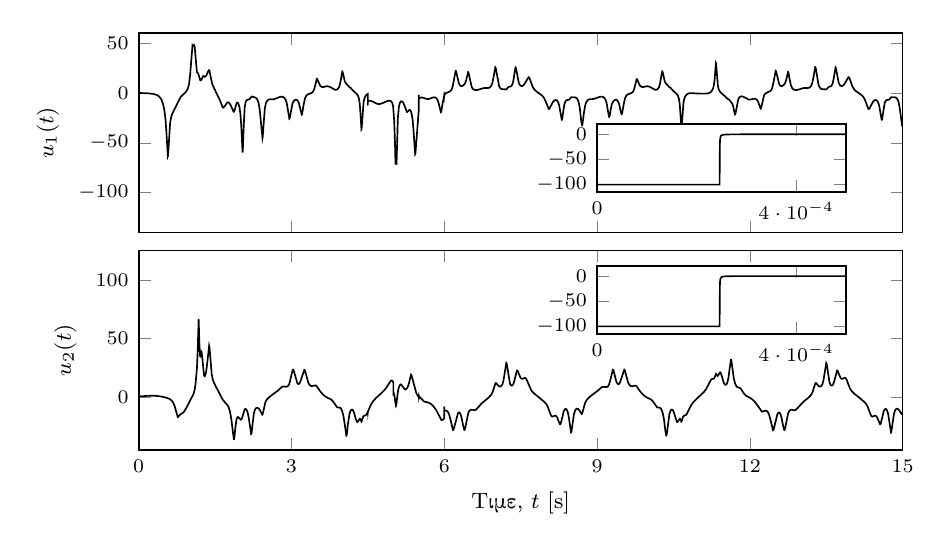
\begin{tikzpicture}

\begin{axis}[%
width=\figurewidth,
height=0.464\figureheight,
at={(0\figurewidth,0.506\figureheight)},
scale only axis,
unbounded coords=jump,
xmin=0,
xmax=15,
xtick={0,3,6,9,12,15},
xticklabels={\empty},
ymin=-140,
ymax=60,
ylabel style={font=\color{white!15!black}},
ylabel={$u_1(t)$},
axis background/.style={fill=white},
xlabel style={font=\footnotesize},ylabel style={font=\footnotesize},ticklabel style={font=\scriptsize},x tick label style={font=\scriptsize},y tick label style={font=\scriptsize},legend style={font=\scriptsize}
]
\addplot [color=black, forget plot]
  table[row sep=crcr]{%
0	-0\\
2.8421709430404e-14	0.603033936428076\\
8.5265128291212e-14	-89.5\\
nan	nan\\
0.000246126881151554	-89.5\\
0.000372079771537415	-0.0224474615202155\\
0.0389836249341613	-0.0632003833495816\\
0.0782663588592101	-0.11979936931246\\
0.123247934159124	-0.209842838714053\\
0.160834106192212	-0.31350496405733\\
0.198420278225299	-0.453798367719315\\
0.236006450258387	-0.647077010498862\\
0.275557525864798	-0.938157048328506\\
0.307444035131482	-1.27628613418047\\
0.336459295351659	-1.71285235840519\\
0.36260330652533	-2.2730718982792\\
0.388747317699	-3.0880400553351\\
0.422668912618704	-4.8091479796133\\
0.450880864497307	-7.26851871856223\\
0.478151286312226	-11.2216497880714\\
0.503174231949032	-17.2182962292815\\
0.525856824501034	-26.6163949586224\\
0.544921130595625	-40.6411253430788\\
0.571457085880908	-63.381027866301\\
0.574399505407314	-62.979646763152\\
0.582337629111791	-57.4372320030107\\
0.616257696851349	-29.9317840182269\\
0.63851531354527	-23.7453039078242\\
0.666167508670824	-19.9691749203709\\
0.824840184062921	-3.84847790534822\\
0.870955092528249	-1.55287602490739\\
0.92736823461172	1.17838200265868\\
0.95473052005984	3.33445411267016\\
0.972496668653079	5.70006911029277\\
0.990262817246304	9.83933666108092\\
1.0098472376618	18.8345506627979\\
1.0559121669781	47.9752273182332\\
1.06616478659993	47.2846791893775\\
1.07067249854313	47.1348405179449\\
1.07558687458082	47.2657352177088\\
1.08879336027479	48.0715970020381\\
1.09462828191224	47.4069590795619\\
1.10338066436839	43.5734091187043\\
1.14176034364328	21.2171799001201\\
1.15563120598333	20.1191996730736\\
1.16565139780721	19.6977214075754\\
1.17552132837331	18.2735677170275\\
1.20785067773313	12.781206145715\\
1.21398562238372	12.648563147546\\
1.21975053702575	12.7261304150199\\
1.22972350799145	13.2293690318156\\
1.24621341342917	14.9661598632365\\
1.26732346031181	17.004456447417\\
1.26905936654659	17.0223883360717\\
1.2742670852509	16.9445143284767\\
1.29797937575469	16.2128917728326\\
1.30229931050577	16.2456723189298\\
1.31142994617537	16.5295370192365\\
1.32769995372114	17.6552202716134\\
1.35555585539707	20.8406995941117\\
1.37774745414212	22.859469559708\\
1.38260210431585	22.7872598767189\\
1.39092218235828	21.8888990615508\\
1.40656826601462	17.8389501028783\\
1.44022809924836	9.5050149398932\\
1.46848648727149	5.92343398575221\\
1.59176274190673	-7.05958009577937\\
1.64767246403025	-14.4043184611395\\
1.65804120134516	-14.7319245918439\\
1.66322557000262	-14.6846531433978\\
1.67625091921728	-14.0310216826166\\
1.74173480519848	-9.43246331382787\\
1.74980545616616	-9.36444748321449\\
1.75384078165001	-9.37908627631113\\
1.76360338325168	-9.54473392348896\\
1.77824728565419	-10.1280741688528\\
1.79801520786593	-11.5332106947023\\
1.82803116969612	-14.9282360447121\\
1.86428452160354	-18.9587765052431\\
1.8672279766205	-18.9699916102831\\
1.87311488665443	-18.6842088215003\\
1.88491997617466	-16.8618935659597\\
1.92350957415945	-9.96326495632853\\
1.93417484631715	-9.61421521426094\\
1.93927060747745	-9.66138512740119\\
1.94741601790307	-9.99497788764381\\
1.96054112894257	-11.2005648265721\\
1.97663504613588	-14.0532058368844\\
1.99424923936755	-19.9892462517076\\
2.01122470518547	-31.1684536689666\\
2.03945699446339	-59.8760774792394\\
2.04376290347213	-57.8403707701097\\
2.05791166582245	-37.2379212000314\\
2.07971167749199	-15.1439078088091\\
2.09712353208329	-9.21252348501663\\
2.11513283671904	-7.31258539647332\\
2.13094367553134	-6.83434371994581\\
2.14539162603573	-6.72045872651243\\
2.15733798478661	-6.63586379479432\\
2.1669377155016	-6.45111569677103\\
2.1789906835382	-5.93584224403544\\
2.21973608566674	-3.46802111989108\\
2.22546063762813	-3.53367156919678\\
2.26621235773325	-4.28177653020921\\
2.28277760112073	-4.45569193687494\\
2.29822867166068	-4.81678872843386\\
2.31527046318563	-5.58650374962686\\
2.33317495203114	-7.05818986066201\\
2.35419209429179	-10.2918107008114\\
2.37561087336805	-16.643244253532\\
2.39663277812807	-27.7696476660451\\
2.42968488574057	-45.2859598908892\\
2.43618883850571	-43.4974680943529\\
2.45035645319182	-32.6549203697937\\
2.47612551808452	-15.4140449133316\\
2.49555509908444	-10.5087930789397\\
2.51917970769681	-7.92753015433716\\
2.54114371539681	-6.87223157301112\\
2.56115778444345	-6.47021643754715\\
2.57574460237346	-6.36965938103565\\
2.58716164824685	-6.35624909039588\\
2.61841572686723	-6.39673696092252\\
2.6249279840373	-6.39087196777118\\
2.63795249837747	-6.34213166677173\\
2.65748926988772	-6.15775131164946\\
2.68396720335558	-5.70553746118598\\
2.77661841616077	-3.8688680644328\\
2.79670030039732	-3.72427483359958\\
2.80413422866411	-3.71461818643571\\
2.81156815693092	-3.73301850479783\\
2.82643601346452	-3.86834973863179\\
2.84130386999813	-4.16734423754946\\
2.86360565479853	-5.06117676089278\\
2.88590743959894	-6.86917971014735\\
2.90778974188359	-10.4175984165904\\
2.92930666183887	-17.0511843557122\\
2.9577912714722	-25.9692898564205\\
2.96100581847681	-25.8422710879724\\
2.96817750450673	-24.4109423738406\\
3.02132407093855	-10.0524917416595\\
3.04706133741215	-8.01058053771327\\
3.07151236860467	-6.9965789611306\\
3.0854305233993	-6.78503167233114\\
3.08821711355026	-6.77775922810429\\
3.09754427781957	-6.8447886000241\\
3.10880622972178	-7.13043011677401\\
3.12435871034495	-7.97023604236263\\
3.14152082522878	-9.71643007359964\\
3.16342305547469	-13.8140890483615\\
3.19984199370212	-21.8659020054863\\
3.2030041534483	-21.7540531084682\\
3.2112022417532	-20.4255279302525\\
3.23427019882337	-12.7780391255033\\
3.26313456376403	-5.63994499612008\\
3.28653565823869	-2.96961757965357\\
3.31048792995153	-1.74956197013317\\
3.33616771663029	-1.11383371280716\\
3.39864126560533	0.124642161680654\\
3.41601959297297	0.875927231387195\\
3.43620039222324	2.53230222143377\\
3.45548264422152	5.64891891556988\\
3.49692281283639	14.2195890490261\\
3.50015455069891	14.1659142212574\\
3.50845979899577	13.4565367804868\\
3.56595249795947	6.96872251288032\\
3.58779828795151	6.20413514899971\\
3.60382255271242	5.98512161568313\\
3.61450539588635	5.95033412159785\\
3.61984681747332	5.95905242022012\\
3.63148186438823	6.02591820694593\\
3.65475195821807	6.28621420150448\\
3.68820935441883	6.67031276857199\\
3.70202929079048	6.73358744549583\\
3.71416573865902	6.71223115997746\\
3.72630218652755	6.61020597725917\\
3.74460022631933	6.30539776983331\\
3.77429962270921	5.50778448631436\\
3.84772469774724	3.39944664432201\\
3.86675371124866	3.19050244479777\\
3.87185269853499	3.18361693421808\\
3.88053713794827	3.23014118691729\\
3.89101124624763	3.39764897815755\\
3.90697160737919	3.93688397559809\\
3.92399244308088	5.02217791667779\\
3.94331238079211	7.30612164069281\\
3.96164793284876	11.3345070084349\\
3.99822514920385	21.5220565328992\\
4.0011119855498	21.3880810423513\\
4.00934983770459	19.9369163935557\\
4.04924667779683	11.1005773212928\\
4.07286233524839	9.4615849308712\\
4.13785032164822	5.8301586246547\\
4.1608206606569	5.06946111974504\\
4.18786138952566	3.44829245181198\\
4.22335645901508	1.57713753436444\\
4.28371643790013	-1.01547105157142\\
4.30727186652803	-3.0000261418969\\
4.32532639016878	-5.87359827308026\\
4.33969546036445	-10.5897529852511\\
4.35525894927343	-21.6390479374863\\
4.37343766752788	-36.5171476418378\\
4.37500093964906	-36.3856118608124\\
4.38055327468851	-33.4336331990083\\
4.41674346275524	-8.75062589148909\\
4.43832856334021	-4.59121080647324\\
4.4617981150716	-2.4580210086451\\
4.48982185994689	-1.12813493136436\\
4.50000030295023	-0.833930470993693\\
4.50008428162512	-12.1744915967123\\
4.50015929417982	-6.99224270690905\\
4.50023008533938	-9.47263942323457\\
4.50030698304154	-8.28013833150278\\
4.50037645291567	-8.8467236365191\\
4.50045313676159	-8.56860974022881\\
4.50052229729826	-8.69639726922799\\
4.50059694548902	-8.62916010836321\\
4.50066766307928	-8.65587873068885\\
4.50074329771013	-8.63748082634211\\
4.53401500963362	-7.80209623015924\\
4.53855867886533	-7.79021976326216\\
4.54310234809704	-7.79646467442745\\
4.55218968656045	-7.85690542729864\\
4.56726973196693	-8.07251018354052\\
4.59348619974276	-8.67885870530934\\
4.67811024065517	-10.8114594853118\\
4.69649365699122	-11.0295633446171\\
4.71487707332729	-11.1101317048322\\
4.72406878149532	-11.0979985944692\\
4.74245219783138	-10.9728182694112\\
4.76813468272606	-10.5972721731453\\
4.8109388242172	-9.62447781876229\\
4.87399055453398	-8.18491443317656\\
4.89971327361005	-7.84049924581217\\
4.91540747996979	-7.74948110465976\\
4.92394995311285	-7.75204644451783\\
4.93249242625592	-7.80398809639827\\
4.94530613597053	-8.01180321864699\\
4.96165888724997	-8.64396550997134\\
4.97780465354201	-10.0123491901404\\
4.99337416024703	-12.7289689332662\\
5.00009744261661	-16.2031081763117\\
5.00015556148077	-17.9484714769178\\
5.00023681724167	-17.0221250868859\\
5.0003150958714	-17.3346308357087\\
5.00037737291643	-17.2547175308467\\
5.000470198751	-17.344904145252\\
5.00259173772341	-18.2788469995639\\
5.01709707424341	-28.2427509756793\\
5.03240782640371	-50.5817382410679\\
5.04160615131062	-71.2755610230492\\
nan	nan\\
5.06219172422215	-72.1794916533924\\
5.08855609078724	-25.0723716330918\\
5.10801312449972	-14.1235584298134\\
5.12809010432588	-9.9344323331749\\
5.14674584799035	-8.55093947416243\\
5.16008008439871	-8.32833536647162\\
5.16756229075349	-8.40486628387058\\
5.17991503088633	-8.82010617988676\\
5.19599108527835	-9.92981041942132\\
5.21689085843731	-12.4735442073989\\
5.26547697786404	-19.0646263086637\\
5.26906829852757	-19.1002276058216\\
5.27355518355797	-19.0328565145139\\
5.28440576269752	-18.5011651719595\\
5.31420997730918	-16.9898643630509\\
5.31594547741147	-16.9791663043811\\
5.32152592606657	-17.028519896138\\
5.33017192274404	-17.3650745156718\\
5.34465000598556	-18.629890071862\\
5.36212176212456	-21.5213334647869\\
5.37828294538798	-26.6735693537319\\
5.39593846064862	-37.3300556263589\\
5.4284126534918	-61.4433889903825\\
5.43104980626363	-61.2188453492949\\
5.43850555024629	-57.6656937183358\\
5.4976537172743	-17.9923202376\\
5.50002458417327	-15.7347320392853\\
5.50009280618309	-1.90001346760707\\
5.50017149278627	-7.46757885102188\\
5.50024896691014	-5.4161874719854\\
5.50032542393127	-6.12671629397863\\
5.50040529546666	-5.89132228420654\\
5.50048195053209	-5.94745190222774\\
5.50061638829973	-5.92297557051941\\
5.52741003561668	-4.7582041275909\\
5.54443800422831	-4.55482714939274\\
5.55174056631132	-4.54665236250366\\
5.55904312839434	-4.57352137594066\\
5.57376839333341	-4.70751055725201\\
5.60423085842164	-5.17893775290437\\
5.65376271348305	-5.96006805496305\\
5.6699587906247	-6.07398929959501\\
5.68075617538581	-6.08373305918657\\
5.6917526828141	-6.03436712338569\\
5.70854612795732	-5.84723954160927\\
5.74003870194738	-5.23905844320494\\
5.78003710023521	-4.49449646998644\\
5.7972822140252	-4.36963233902358\\
5.80877895655186	-4.39551403943936\\
5.82027569907852	-4.53132660172571\\
5.83442018326502	-4.88808141825069\\
5.85171218970414	-5.71149528268562\\
5.87111273932888	-7.41122488575132\\
5.89161739618045	-10.6592644014051\\
5.93257878799542	-19.3368094583789\\
5.93594811399876	-19.2315173629219\\
5.94366985430213	-18.026274284266\\
5.96523906962544	-10.9537116812658\\
5.99095295533797	-4.62504880725396\\
6.0001019406283	-2.07215786798807\\
6.00013905985354	-1.43117290315587\\
6.00021044481377	-2.19689599929315\\
6.00027446026623	-1.86441267465401\\
6.00033735917513	-2.0532642671299\\
6.00040455686626	-1.90906518143355\\
6.00046621140088	-1.9960483586385\\
6.00053618907214	-1.93099905195774\\
6.00059741129404	-1.96325015714501\\
6.00066558034761	-1.93287593283459\\
6.00072098925131	-1.94340733324638\\
6.00080391786668	-1.92682092488634\\
6.03281721603021	-0.203497080829507\\
6.06114023802222	0.473725685685423\\
6.11060571679887	1.54059159514425\\
6.13035720796444	2.42763161498283\\
6.14832677125058	3.95306560687898\\
6.1676223623282	7.00104612009724\\
6.191293018021	13.5266277953211\\
6.22247041613774	22.0664104294849\\
6.22554977541004	22.1391325051927\\
6.23016881431849	21.8633626210543\\
6.2411834705085	19.7279567584893\\
6.28724739439605	9.44778187483936\\
6.31023228738377	7.51690290233449\\
6.32890690281243	6.90807896707445\\
6.33814342390345	6.83626226699018\\
6.34390239029779	6.85703204402786\\
6.35350066762169	6.99287449805203\\
6.36966728401264	7.46763556086458\\
6.39451450744714	8.66739828597453\\
6.4135131118182	10.2271060690085\\
6.43188814459972	13.1404366189022\\
6.46838436555333	21.0716017333015\\
6.4719645830576	20.9517911591319\\
6.48032063869447	19.5427215506809\\
6.53962974426133	5.72481956319189\\
6.56532709660061	3.96245310404369\\
6.58745371615954	3.25128204175897\\
6.60635303368402	2.97516280495468\\
6.62229016060321	2.90553994211994\\
6.63176387693719	2.91959391478986\\
6.6454670068823	2.99962448081125\\
6.66672377802978	3.23397909860809\\
6.70092543837762	3.79108829703526\\
6.76332370784957	4.80374130225496\\
6.78424890545639	4.9662443109888\\
6.79946708718886	5.00568830894743\\
6.81492288008386	4.99222798869287\\
6.84678491052404	4.9323716924841\\
6.85744062532864	4.95667061701694\\
6.8721889594201	5.08091570579082\\
6.88841928460269	5.4053270153593\\
6.90504877043621	6.05216857312244\\
6.92285566155438	7.30439383557274\\
6.94238956623077	9.7960527896031\\
6.96298334463125	14.5574014044418\\
7.0022764769945	25.9198751198425\\
7.00625962946002	25.7625893791566\\
7.0147084500626	24.0871395538429\\
7.07818409564845	6.54886443503345\\
7.10277250032605	4.65309824033095\\
7.12297097813185	3.96424773402175\\
7.14173173400843	3.7223555568485\\
7.15103146662302	3.6969640754666\\
7.16265613239126	3.71876357277178\\
7.1789580978048	3.76024702560402\\
7.18552121571763	3.74392278927785\\
7.19535201640319	3.65430716576999\\
7.21190816224005	3.47914585861491\\
7.21558730575934	3.50614384766288\\
7.2240199391298	3.76337816088679\\
7.24223112231472	5.04002642643513\\
7.26350084401612	6.10671457809295\\
7.27770197352005	6.29016532265484\\
7.29683666297458	6.4389960792346\\
7.3086973458995	6.70815232307163\\
7.32410712930012	7.476591533093\\
7.34070391571848	9.16751151168155\\
7.35883603430075	12.7875037658174\\
7.38081933987685	20.684827808352\\
7.4000435986413	25.7112908714861\\
7.40379550284607	25.5513320357877\\
7.41254994599053	23.7473498797254\\
7.46548258719311	9.82091105262951\\
7.48844197253472	7.74358939007361\\
7.50799115318942	7.02851191297836\\
7.51925555578275	6.92487944323177\\
7.52321237356156	6.93407563038745\\
7.53112600911919	7.01892558515388\\
7.54700805096253	7.44416195271896\\
7.56706599349701	8.44930963918476\\
7.59436410027921	10.6067368569954\\
7.65615611537449	15.9107462892121\\
7.66000019877954	15.8586130992807\\
7.66789470942915	15.4492525811494\\
7.68372998047761	13.559385460049\\
7.74401660236619	5.25765333800388\\
7.77499176950248	3.10711625447557\\
7.81704064945095	1.25408054512401\\
7.92971961526699	-2.9914847217472\\
7.96189728054924	-5.16386112473084\\
7.99014290014833	-8.29610037211387\\
8.05221444221169	-16.1720141365384\\
8.05697162991937	-16.1020564793671\\
8.06744970658018	-15.528425281644\\
8.09465285084472	-12.7566438476489\\
8.13659443530707	-8.89151394353608\\
8.163020649503	-7.51661692391257\\
8.18243983177916	-7.0992174153681\\
8.1863961102335	-7.0789816688022\\
8.1943086671422	-7.10900831520208\\
8.20617750250524	-7.34653634055684\\
8.22031149765691	-7.98834696472296\\
8.23682056171666	-9.39876025471681\\
8.25658197325335	-12.4920230699815\\
8.27828925833175	-18.5527079939373\\
8.30749227331319	-26.9697802724074\\
8.30877273071681	-26.960721508252\\
8.31389456033128	-26.3867234390505\\
8.32626216635131	-22.2716971780349\\
8.35816389349694	-11.4188565005471\\
8.37966551807001	-8.40138792673459\\
8.39975800222976	-7.2745501472783\\
8.41630438644553	-7.00025035328431\\
8.42713851925276	-6.97882057952819\\
8.437404340629	-6.9595677461062\\
8.44512633289025	-6.86949702290298\\
8.45494778785337	-6.56268179132559\\
8.47213125482537	-5.42790591790589\\
8.49326988533019	-4.30913509571451\\
8.49827104833049	-4.27241967514028\\
8.50502838506021	-4.30894378803302\\
8.52485388577496	-4.44263372691007\\
8.53392149651225	-4.42019320100687\\
8.55688714122515	-4.33824655089813\\
8.56397718277849	-4.35882785893581\\
8.57436845364087	-4.46066945292671\\
8.58829577895145	-4.77102967888086\\
8.60407929718241	-5.4536502829729\\
8.62171900833377	-6.84982608113209\\
8.64240635610581	-9.95295484814122\\
8.66129991195484	-15.2029544081268\\
8.68942208844378	-28.0049167275984\\
8.70581183477746	-32.282386835402\\
8.70908463346066	-32.1412037485451\\
8.71699970740396	-30.4336673015417\\
8.74058264751206	-20.5174706792037\\
8.76754215498569	-12.4021583901123\\
8.7925283841959	-8.81901276505992\\
8.81653396963944	-7.19891239250117\\
8.83854251928302	-6.52007629559009\\
8.85750806303247	-6.27464770793392\\
8.87521201800345	-6.19344044970978\\
8.90784562975938	-6.12069577292894\\
8.92676429578326	-6.00175973706533\\
8.94939778430827	-5.73082405576044\\
8.98511389732997	-5.07641556009078\\
9.04563880165736	-3.96127271808945\\
9.0691834082261	-3.73153233149617\\
9.08182390271961	-3.69210405916752\\
9.09115991753052	-3.71030794467408\\
9.10144738319096	-3.78546449891081\\
9.11638858267814	-4.01991338739327\\
9.13456771086707	-4.57190585531136\\
9.15231932891773	-5.53445704592542\\
9.17281449969835	-7.5403337740798\\
9.19224068604782	-11.057103440968\\
9.21502512529543	-18.2949347878362\\
9.23715104798455	-24.1561408177861\\
9.23832598056488	-24.1797106063494\\
9.24067584572555	-24.1100522349829\\
9.24685326270173	-23.2367348782816\\
9.26552034451248	-17.4518421618412\\
9.2916263006024	-11.1917750756706\\
9.31468767768609	-8.75422540148372\\
9.34210419587667	-7.29412935527122\\
9.3630868333134	-6.79088809218835\\
9.36952074946143	-6.75593648158711\\
9.37607894801683	-6.78412432633138\\
9.38515463251036	-6.93819029562937\\
9.39865248893955	-7.45092053320734\\
9.41685506230935	-8.83967467876602\\
9.43663526793124	-11.6856719122453\\
9.46227281491629	-17.937900758929\\
9.48110014329595	-21.3349533086882\\
9.48252839512419	-21.3616244317248\\
9.48538489878068	-21.2851604584238\\
9.49299328944954	-20.2616770097744\\
9.51053347592379	-15.0409469373713\\
9.5442086600296	-6.12825762885656\\
9.56724986194455	-3.26756306532072\\
9.58998563791326	-1.958267135299\\
9.61554586999577	-1.24648484975648\\
9.68959617027163	0.332795031861167\\
9.70959046635942	1.4763565813215\\
9.72817780580843	3.5674256786247\\
9.74768345297373	7.62282468269149\\
9.77774461840714	13.9247561718565\\
9.7811589244683	13.9848401895567\\
9.78537319427222	13.8368407904243\\
9.7962453011416	12.6684181000291\\
9.83792064227096	7.660416003694\\
9.86090984711282	6.49106460366468\\
9.88033273631241	6.07101899008003\\
9.89480890609528	5.97773850706162\\
9.90142178336015	5.98120290486447\\
9.91257471328507	6.03758416213159\\
9.93166405675572	6.23561360851291\\
9.97639374112163	6.73354196331353\\
9.98899834586457	6.76558125315597\\
9.99455898641705	6.75416019851947\\
10.005680267522	6.68025139376931\\
10.0244071059012	6.4013062169017\\
10.0515700932908	5.70924088029017\\
10.135079845905	3.33274081390178\\
10.151439382346	3.18326156102967\\
10.1604065532457	3.19892099096197\\
10.1696153653684	3.30278378024164\\
10.1825381581268	3.62560239324637\\
10.2004347773916	4.50924332729451\\
10.2180292502764	6.12108658849725\\
10.2372615999134	9.39847777334622\\
10.2586382420274	16.0307757483368\\
10.2808544652088	21.6690028963715\\
10.2843270151162	21.5290803439681\\
10.2927439772175	20.0043499473554\\
10.3335024431613	10.9981943339947\\
10.3575538677356	9.34739649665607\\
10.4176183062926	5.91608988680647\\
10.4435735157187	5.10141743221061\\
10.4683771267954	3.64546439134475\\
10.5073249945363	1.56456749581933\\
10.5678733819358	-1.06578524055953\\
10.5909178279563	-3.03201197619187\\
10.6083716506375	-5.80208677237901\\
10.624056163109	-11.0722093813957\\
10.6392422461699	-22.2664110700513\\
10.6567228431158	-36.1375418724805\\
10.6582779715069	-35.9699248847678\\
10.6641427462959	-32.6969956935084\\
10.6990344227522	-8.90711474141072\\
10.7201246423822	-4.70421545928988\\
10.7444485196271	-2.44783868825618\\
10.7719451214659	-1.12842525339845\\
10.7981229465278	-0.49963393083334\\
10.8200741449915	-0.260553883820748\\
10.8383311897807	-0.184540415357063\\
10.8529297014926	-0.174631760348618\\
10.8726203860337	-0.206037871372587\\
10.9030540191836	-0.306535111472357\\
10.9635779011737	-0.515804172211077\\
10.9955262064736	-0.583615861981258\\
11.0275294844123	-0.623813994354165\\
11.0719456085502	-0.655033441350227\\
11.0992570870401	-0.660571313335453\\
11.1158973096395	-0.652853079204746\\
11.1309701025116	-0.632565173464741\\
11.150661510262	-0.57403168195242\\
11.1688940272335	-0.465927518946728\\
11.1872806863048	-0.270074288151534\\
11.2107125155844	0.183419741285164\\
11.2341002982119	0.985791885579602\\
11.2566245735122	2.27849379970091\\
11.2778054773832	4.43207359565356\\
11.2939030187558	7.58498483181215\\
11.3098469717169	14.0411969007829\\
11.3344103177505	30.079610962947\\
11.3373777083947	29.7692778283281\\
11.3445117332802	25.4476821150628\\
11.3723904628281	7.43034112093338\\
11.3920898647084	3.39918477411361\\
11.4161914137192	1.17216238827204\\
11.446958232712	-0.441814167746628\\
11.5156985653234	-3.41958029922912\\
11.5564323592281	-5.61603819257307\\
11.6023773741004	-7.11461960911068\\
11.656806255863	-10.840519251231\\
11.6722705839712	-12.9953766713051\\
11.6927361015623	-18.2980286092796\\
11.7096656881877	-21.6024373213304\\
11.7135612233669	-21.4523278976825\\
11.7215248319978	-19.8867281119979\\
11.7751240486201	-5.98567493770156\\
11.7988053056126	-4.16670216042408\\
11.8198521698085	-3.49343619515848\\
11.835567414469	-3.36087288217652\\
11.8456101544767	-3.40163892946369\\
11.8597922819471	-3.58767087774942\\
11.8839460890315	-4.14304639648586\\
11.9762554098691	-6.55049001157602\\
11.9924623446954	-6.66196285069144\\
12.0015077885066	-6.66170277513585\\
12.0105532323178	-6.62061585101355\\
12.0289087038022	-6.43804370779573\\
12.0818316663154	-5.80278193583955\\
12.0915113174784	-5.7791457500563\\
12.0963511430599	-5.78860391047839\\
12.1082613581398	-5.88548121646886\\
12.121322972522	-6.14134601557683\\
12.1383740924207	-6.79836675441516\\
12.1586899019056	-8.29566571742259\\
12.1811388559384	-11.3101310736616\\
12.2132313557945	-15.7574276717167\\
12.2178533920179	-15.529389647252\\
12.2270974644647	-13.9757716533435\\
12.2814984352499	-2.15595075948561\\
12.3053082244739	-0.599939006228666\\
12.3303496277082	0.188331416549175\\
12.4047483713828	1.97068381347587\\
12.4223308906412	3.0666339863927\\
12.4416964228228	5.3538831222611\\
12.4613839278689	9.55670754116699\\
12.5082538657538	22.2168625349996\\
12.5117757165612	22.0824335278326\\
12.5206850872106	20.6897708407424\\
12.5796807711002	8.50471957868584\\
12.6018981926206	7.18153516875196\\
12.6174890680414	6.87505255181142\\
12.6214940360954	6.86150412135765\\
12.6268820748725	6.88098100710636\\
12.6359437299786	7.00430833213143\\
12.6530152981501	7.50228667861438\\
12.6775981926062	8.69534735783131\\
12.6972393221247	10.3300287956347\\
12.7150955153497	13.2003300914222\\
12.7515040942506	21.1648010266556\\
12.754556315166	21.0872390096678\\
12.7613590727399	20.1292547306042\\
12.7807845483614	14.1779877386943\\
12.8080361215347	7.63209347802673\\
12.8305313573958	5.07016826772967\\
12.8529475613312	3.79734052503737\\
12.8757298526591	3.17086706894352\\
12.8945412714786	2.95694660388033\\
12.9061922606371	2.92289875725007\\
12.9197709021379	2.958316661106\\
12.9350931021001	3.07700284268707\\
12.9596951752152	3.3974256252759\\
13.0137145743786	4.3566602895839\\
13.0502223262445	4.87573519268956\\
13.071997118483	5.0207455622744\\
13.0834063174391	5.0429367523613\\
13.0991870600635	5.02737021690926\\
13.1297874871191	4.969822766281\\
13.1399333486486	4.99118274895153\\
13.150079210178	5.05876827693807\\
13.1664099123717	5.31249346644704\\
13.1838928001772	5.88335877124295\\
13.2028490253739	7.06594625500817\\
13.2226062432542	9.36296293843499\\
13.2437989013046	13.9287596055968\\
13.2855760446577	26.0082812157629\\
13.2869641177807	25.9983790714489\\
13.2911283371496	25.6504417069824\\
13.3021356627242	22.7924040104713\\
13.34909279411	8.2769491712463\\
13.3717396297177	5.57732174698096\\
13.394642587264	4.30428312182373\\
13.4151774168395	3.82518919319644\\
13.4292177727968	3.71897789122013\\
13.4362379507754	3.71212238847886\\
13.4507097665107	3.75158420817645\\
13.4626150641197	3.77747551256675\\
13.4697582426852	3.7568787050652\\
13.4821874084831	3.62567675988377\\
13.4947493169454	3.50293466344664\\
13.500347174696	3.55739180275071\\
13.5090188737037	3.88240276554411\\
13.5577984677322	6.28651289620814\\
13.5834533088273	6.51004968498978\\
13.5964420615156	6.89071777563423\\
13.6119932160703	7.85847166839775\\
13.6297197941121	10.0969361077249\\
13.6473493226175	14.3783078458332\\
13.6839323307301	25.742345156285\\
13.6876328493279	25.5078368087214\\
13.6967447318717	23.4685481862676\\
13.7451517147417	10.3124496770119\\
13.7691138569141	7.89980975122134\\
13.7888921449304	7.0783452400965\\
13.8026430240589	6.92829306989019\\
13.8122881019646	6.99240134031601\\
13.8260779061246	7.30547733004353\\
13.8445547697855	8.11539088972044\\
13.8723099981409	10.1325772049981\\
13.9382084396517	15.9190242123558\\
13.9440745473218	15.8441221386401\\
13.9538135919157	15.2265812722958\\
13.9713572932272	12.8719322321942\\
14.021410201164	5.80255544303398\\
14.0521905275824	3.45459858102303\\
14.090387479425	1.63448786951257\\
14.1547486754295	-0.604663726088887\\
14.2025595048796	-2.46525003461818\\
14.2312615102855	-4.08499041119134\\
14.2593550652705	-6.54067155151056\\
14.2883954943603	-10.5707334092108\\
14.3279618909009	-15.9591952772675\\
14.335604563883	-16.140643495883\\
14.3406996792043	-16.0559109066616\\
14.3512088903136	-15.4577505839911\\
14.3782716900836	-12.6929329783462\\
14.4193781685772	-8.91080487528536\\
14.4462797572069	-7.50722259453572\\
14.4637916201263	-7.10973829069428\\
14.4708264180488	-7.07082525142995\\
14.4796032217388	-7.12693175025136\\
14.4913297711073	-7.40344550371046\\
14.5060784995001	-8.1478625690262\\
14.5238163715345	-9.84550793647757\\
14.544183827095	-13.4538189042263\\
14.567939831098	-20.8785777545822\\
14.5899892055016	-26.899513798438\\
14.5913229556266	-26.9183799261713\\
14.5953242060016	-26.6234116467628\\
14.6046209417871	-24.1422800321931\\
14.6489258710367	-10.0267834681654\\
14.6708955987629	-7.78662228973931\\
14.6898485013309	-7.08450589770416\\
14.7039528369429	-6.9572771143647\\
14.7182769673895	-6.93999581630214\\
14.7262597012664	-6.8710227650882\\
14.7356372028964	-6.62944830722489\\
14.7494262713743	-5.8386058659616\\
14.7764782819866	-4.26875347702143\\
14.7818150942782	-4.23453043449796\\
14.788054657268	-4.27247076080575\\
14.8084087997741	-4.41634485809404\\
14.8188669150698	-4.38897146646325\\
14.8386950295194	-4.31841913423057\\
14.8472985886091	-4.3407281123109\\
14.8574436509956	-4.44061059836147\\
14.8728014402159	-4.79418708115469\\
14.8896303570778	-5.57496624861801\\
14.9075506892122	-7.11620847886013\\
14.9272694507019	-10.2762848314531\\
14.9474058213132	-16.2525679450243\\
14.9891993205763	-32.2093302966594\\
14.9918589451348	-32.1035293915337\\
14.9987829342858	-30.7842449021551\\
15	-30.4187342271749\\
};
\end{axis}

\begin{axis}[%
width=0.326\figurewidth,
height=0.158\figureheight,
at={(0.60\figurewidth,0.6\figureheight)},
scale only axis,
xmin=0,
xmax=0.0005,
ymin=-115,
ymax=20,
xtick = {0, 4e-4},
scaled x ticks = false,
axis background/.style={fill=white},
xlabel style={font=\footnotesize},ylabel style={font=\footnotesize},ticklabel style={font=\scriptsize},x tick label style={font=\scriptsize},y tick label style={font=\scriptsize},legend style={font=\scriptsize}
]
\addplot [color=black, forget plot]
  table[row sep=crcr]{%
0	-0\\
2.8421709430404e-14	0.603033936428076\\
2.22695760498937e-07	-100\\
0.000246078065231359	-100\\
0.000246628866975129	-19.7755725436816\\
0.000247149861422713	-9.47139255396654\\
0.000247670855870297	-5.97732791297092\\
0.000248403529539587	-3.81247319704084\\
0.000249136203223088	-2.741600431772\\
0.000250174720690666	-1.92196015979735\\
0.00025151908194232	-1.35640269532834\\
0.000252863443208184	-1.03000954158391\\
0.000254419968712227	-0.791687836039884\\
0.000256188658468659	-0.614626934897586\\
0.000257957348225091	-0.492546272705226\\
0.000259829200430772	-0.398769809883717\\
0.000261804215099914	-0.324880753437512\\
0.000263779229769057	-0.268216301551348\\
0.000265754244423988	-0.223672877529211\\
0.000268096863180745	-0.182218155206556\\
0.000270439481937501	-0.149892684517312\\
0.000272782100680047	-0.124410194941206\\
0.000275124719436803	-0.104178132454052\\
0.00027746733819356	-0.0880392812542254\\
0.000279809956936106	-0.075125997557862\\
0.000281942490730103	-0.065611232032424\\
0.000284590848977473	-0.0561595681471232\\
0.000286768577197449	-0.0499614471997347\\
0.000288946305431637	-0.0449020242699731\\
0.000291806380388948	-0.039639623266595\\
0.000294666455360471	-0.0356064400159966\\
0.000296841648633972	-0.0331823531574287\\
0.000299285318547504	-0.0309844908224903\\
0.000301728988461036	-0.0292336198834846\\
0.000304172658388779	-0.0278390197651817\\
0.000307229836863598	-0.0264870817421041\\
0.000310287015324207	-0.0254705772210855\\
0.000313344193799026	-0.0247065687266996\\
0.000314872783036435	-0.0243990887509682\\
0.000316686345172457	-0.0240870350368567\\
0.000318499907294267	-0.0238237853521923\\
0.000320313469430289	-0.0236017568544895\\
0.0003221270315521	-0.0234145479797263\\
0.000323940593688121	-0.0232567533043664\\
0.000325754155809932	-0.0231238021113569\\
0.000327567717945954	-0.0230118271918514\\
0.000329785001767391	-0.0228987080786567\\
0.000332002285574617	-0.0228071467397797\\
0.000334219569396055	-0.0227331104393897\\
0.000336436853217492	-0.0226733216732384\\
0.00033865413703893	-0.0226251168937779\\
0.000340871420860367	-0.0225863295980702\\
0.000343088704667593	-0.0225551953549257\\
0.000345565465153186	-0.022527711833078\\
0.000348042225624567	-0.0225063838695263\\
0.00035051898611016	-0.0224899391279649\\
0.000352995746581541	-0.0224773683404464\\
0.000355472507052923	-0.0224678670844298\\
0.000357949267538515	-0.0224607982636513\\
0.000360426028009897	-0.0224556598654004\\
0.000364310609185736	-0.0224505618490554\\
0.000368195190361575	-0.0224480998168843\\
0.000372079771537415	-0.0224474615202155\\
0.000375964352699043	-0.0224480862165564\\
0.000379848933874882	-0.0224495846628372\\
0.000383733515050722	-0.0224516916274524\\
0.000387618096226561	-0.0224542182612311\\
0.000392988441930697	-0.0224581647235169\\
0.00040372913333897	-0.0224669597297833\\
0.000419840170465591	-0.0224810636652393\\
0.000475254445149176	-0.0225306832928709\\
0.000514886032988215	-0.0225662623588647\\
};
\end{axis}

\begin{axis}[%
width=\figurewidth,
height=0.464\figureheight,
at={(0\figurewidth,0\figureheight)},
scale only axis,
unbounded coords=jump,
xmin=0,
xmax=15,
xtick={ 0,  3,  6,  9, 12, 15},
xlabel style={font=\color{white!15!black}},
xlabel={Time, $t$ [\si{\second}]},
ymin=-45,
ymax=125,
ylabel style={font=\color{white!15!black}},
ylabel={$u_2(t)$},
axis background/.style={fill=white},
xlabel style={font=\footnotesize},ylabel style={font=\footnotesize},ticklabel style={font=\scriptsize},x tick label style={font=\scriptsize},y tick label style={font=\scriptsize},legend style={font=\scriptsize}
]
\addplot [color=black, forget plot]
  table[row sep=crcr]{%
0	-0\\
6.53699316899292e-13	-60.5\\
nan	nan\\
0.000233286350436401	-60.5\\
0.000233779483806984	100\\
0.000348042225624567	0.571389593767975\\
0.0651721142175319	0.771963237567434\\
0.179627192208756	1.12603399949147\\
0.217213364241843	1.19740273975626\\
0.236006450258387	1.21665723389975\\
0.255781988061599	1.22292602471421\\
0.275557525864798	1.21364337500032\\
0.307444035131482	1.16427335722112\\
0.336459295351659	1.08232448299196\\
0.375675312112165	0.918226066588716\\
0.422668912618704	0.646442341690857\\
0.472695561892749	0.264107250694693\\
0.519597716701767	-0.210487238363939\\
0.571457085880908	-0.904455981811381\\
0.601753604880074	-1.45559503332895\\
0.628608632180118	-2.19537177150333\\
0.655562682377663	-3.33142948742932\\
0.682074748110551	-5.13722941592297\\
0.707567906936731	-8.03085400958422\\
0.766558440621992	-16.9793623857974\\
0.774582036051299	-16.8473202559069\\
0.797010799217119	-15.5438268994069\\
0.821504932064727	-14.6362440513905\\
0.86716518492679	-13.4429355409885\\
0.892990308213669	-12.1394765934437\\
0.934243819891336	-9.16199464790689\\
1.07558687458082	2.73458519361493\\
1.09754574273094	6.1604211136291\\
1.11703751383091	11.9375403269558\\
1.14367846207277	25.0850870005413\\
1.15763813107954	39.1935398303367\\
1.17552132837331	66.5311353189521\\
1.17792871524897	65.6488021948294\\
1.18866557051985	48.0764913038075\\
1.20356930136974	35.3706889595599\\
1.20893880943754	34.8309211520115\\
1.21220320455076	35.0707532513272\\
1.23155300126469	38.5246791452773\\
1.23521198781118	38.228936298592\\
1.24281599462074	35.6501911217561\\
1.28199617744254	18.5777355218146\\
1.29390482408732	17.7767252861598\\
1.29797937575469	17.8555270590449\\
1.30686462834058	18.5542091326263\\
1.32184760886565	21.2429988270537\\
1.34029394788291	27.2207537715331\\
1.38260210431585	43.9788567362799\\
1.38895793137308	42.8475933615636\\
1.40089011610513	36.4917915321455\\
1.43280998783673	19.4931661235838\\
1.45565213223369	14.7474426452517\\
1.48494173448006	11.5910497225041\\
1.64767246403025	-2.03531876997782\\
1.68726493135101	-4.21532868951584\\
1.74577013068232	-7.0052708378706\\
1.76848468405252	-9.00346800525939\\
1.79301254756089	-12.5659591397299\\
1.81802584908606	-18.7763106702841\\
1.8672279766205	-35.8651077855053\\
1.87017143163747	-35.8513560424733\\
1.87827375029721	-34.3835800575908\\
1.89960112338797	-25.206016791254\\
1.92193773725936	-18.6836529115734\\
1.93927060747745	-17.0735630914454\\
1.94741601790307	-16.9535465988766\\
1.95298453261194	-17.0292558390058\\
1.96557885982966	-17.5281830013586\\
2.00357129286954	-19.2424840652972\\
2.00867356774683	-19.1930052253239\\
2.0188781175014	-18.7369668599809\\
2.03298893155218	-17.1708711242501\\
2.08144792376659	-10.3250229583108\\
2.09363457558565	-10.0744770856952\\
2.0988680103321	-10.1060758652866\\
2.10832600030258	-10.3590461311301\\
2.12288131569808	-11.2716222059556\\
2.14126364017734	-13.5424602546746\\
2.16211652828696	-18.1922597562841\\
2.20748000699365	-31.4025148678577\\
2.21015501752404	-31.310534605683\\
2.21718666242489	-30.0938811318956\\
2.23387956082961	-23.3512510192841\\
2.26174475805196	-13.6699886628706\\
2.28277760112073	-10.6314645807033\\
2.30372702942415	-9.37673807415219\\
2.31815632162599	-9.08649978955405\\
2.32566563682857	-9.06766817462984\\
2.33317495203114	-9.12496396225325\\
2.34552829531026	-9.36713897458422\\
2.36480386139434	-10.0961422093101\\
2.38579846027379	-11.4930728259032\\
2.42496315608165	-15.0464583908412\\
2.42968488574057	-14.8814362537567\\
2.43973074217723	-13.4334651159423\\
2.48896700048034	-3.9681135668035\\
2.51661019738441	-2.00890674021198\\
2.55751107996095	-0.147280336359756\\
2.61841572686723	1.94612362831418\\
2.73239970418338	5.56384768014998\\
2.81156815693092	8.77863622609179\\
2.83386994173132	9.07631147714028\\
2.84130386999813	9.09512070915571\\
2.84873779826492	9.0841781226933\\
2.87103958306533	8.96155130808197\\
2.88590743959894	8.89568895319007\\
2.89334136786573	8.89231890777371\\
2.90340494925543	8.93592732242354\\
2.91648599432588	9.10340542295526\\
2.93187988475505	9.53750879557512\\
2.9465806834223	10.3822737903589\\
2.96387449288878	12.3557450876303\\
2.9916845641845	17.6380428349988\\
3.0237647970612	23.2233868840304\\
3.03141278848399	23.4675224396315\\
3.03651144943251	23.2789674495463\\
3.04706133741215	22.089282529165\\
3.11631419765659	11.7115295379997\\
3.13293976778687	11.1818586275123\\
3.13723029650782	11.1693065421863\\
3.14581135394974	11.2980132037101\\
3.16042723842422	12.0146288147165\\
3.17840214072706	13.8271739308221\\
3.2523461437797	23.3043798808445\\
3.2558359155626	23.2482511649797\\
3.26313456376403	22.7812412614478\\
3.27758249745352	20.7127557287365\\
3.33109693081141	12.1329820707672\\
3.35700723474415	10.3143519370611\\
3.3795547481828	9.62331029284081\\
3.39482396212082	9.47019088883125\\
3.40245856908984	9.4620518358676\\
3.41149925167859	9.49654983813799\\
3.43123556069789	9.67652254608366\\
3.46557620220214	9.98023436197282\\
3.47258739647175	9.96224174602609\\
3.48091979642837	9.84608534931401\\
3.49159768076004	9.48986702771245\\
3.51364626125039	8.12769344339705\\
3.57420468216201	4.30835027618794\\
3.62566434093078	1.95953577608317\\
3.67438941804718	0.291142571444666\\
3.71416573865902	-0.647464963737391\\
3.77429962270921	-1.91095822120803\\
3.80325997694811	-2.99418520181324\\
3.83311383410276	-4.73660369031374\\
3.89420331847394	-8.51716160573622\\
3.9101636796055	-8.81681108859685\\
3.92399244308088	-8.87680479598288\\
3.93782120655626	-8.89654933918625\\
3.94856783839109	-8.97983085291234\\
3.95954057517613	-9.20946482950451\\
3.97392769521238	-9.87947388913246\\
3.9920288196289	-11.5687414778496\\
4.01657849153821	-15.3637248650909\\
4.0371238869219	-20.7321790200368\\
4.07620102459305	-32.8623875497118\\
4.07953971393771	-32.7310150423426\\
4.08713198862606	-31.2967341738222\\
4.10821901887491	-23.0964335764934\\
4.1363967620498	-14.6376445143109\\
4.15874857898376	-11.6099470237833\\
4.17799002406903	-10.6343497058621\\
4.18457093437345	-10.5661219696504\\
4.18786138952566	-10.5789003090787\\
4.19457333437222	-10.7003792576758\\
4.2082592931496	-11.3460143266235\\
4.22748355225349	-13.1828527175414\\
4.25920517360503	-18.1584036337477\\
4.28371643790013	-21.0524350560174\\
4.29021720875124	-21.2242935222683\\
4.29517873451425	-21.1720775416789\\
4.30544557653894	-20.6589652752066\\
4.34194548733596	-18.349542425293\\
4.34696006095947	-18.4557477902598\\
4.35635868224121	-19.2227492599333\\
4.37285521419646	-20.999715872675\\
4.37656421177024	-20.8275634424325\\
4.38737419486735	-19.1198729170079\\
4.40803525749874	-16.5794960979314\\
4.42364639484049	-15.9967849556913\\
4.4617981150716	-15.2179186791295\\
4.47967238474634	-14.2315068587374\\
4.50013921049451	-12.2767355833225\\
4.50021592479621	-12.4397056424746\\
4.50029653992327	-12.3354754747522\\
4.50037044730334	-12.3750475751108\\
4.50045976349101	-12.3433527643065\\
4.51085096381264	-11.1902816426532\\
4.56224305016477	-6.18866435192592\\
4.60570568087718	-3.30954175501412\\
4.66008512796304	-0.706141205835294\\
4.76813468272606	3.53499693280278\\
4.83264499328892	6.3554905262216\\
4.87399055453398	8.86011862831134\\
4.95384860911359	14.1513744206089\\
4.96342840803239	14.2451686687117\\
4.97024825090671	14.1786796751881\\
4.98091574866876	13.8523875654707\\
4.9980548340084	12.7634481320278\\
5.00001831497623	12.0515849344033\\
5.00008885653436	1.38302084059632\\
5.00016162014897	5.48770031329163\\
5.00023681724167	3.59104885845331\\
5.00030725039497	4.49655285067642\\
5.00038592719137	4.06722930878244\\
5.00045928128708	4.25397984830597\\
5.00053095275267	4.1604505198318\\
5.00060597076522	4.19496703938353\\
5.00068947966454	4.17027458635022\\
5.00801935400831	3.48437797017014\\
5.02329818685611	0.948797219578069\\
5.04043368848666	-4.8277008749497\\
5.05170250528985	-7.66233724579325\\
5.05399013906913	-7.50003379650263\\
5.06043099441104	-5.57727847476126\\
5.09469774171511	6.21554704684381\\
5.12054567850271	9.7916322678917\\
5.13821577003233	10.8735404366538\\
5.14242729593876	10.9273111784251\\
5.14890512401615	10.8531734831188\\
5.16008008439871	10.3435321410437\\
5.22532217886112	6.57867812352222\\
5.23193212587435	6.53572339703926\\
5.23854207288758	6.56645258823772\\
5.24931603487816	6.76966786847278\\
5.26547697786404	7.42647328939221\\
5.28440576269752	8.84895618430406\\
5.30379697669542	11.4645264118839\\
5.34794019357297	19.282089008173\\
5.35123038116039	19.1798604603339\\
5.35999438126304	18.1406121718709\\
5.44900584215715	3.71795515898384\\
5.4744806781285	1.49943805348381\\
5.50001785511387	0.0289818952917642\\
5.50012918363818	1.77976049565957\\
5.50020714681855	0.461697347843412\\
5.50027900781393	1.31401629011776\\
5.5003544507566	0.810450583307542\\
5.50042655548506	1.08239113388788\\
5.50049352315395	0.933359796481184\\
5.50056473697032	1.00649303454971\\
5.50063688387974	0.963794798538771\\
5.50070299683026	0.981446772713042\\
5.50077489228744	0.967474390683961\\
5.51160271394828	0.468983604138927\\
5.60035316218351	-3.62242110412831\\
5.62562791472463	-4.01956499766243\\
5.6699587906247	-4.41616918868409\\
5.69735049786183	-4.77160213937341\\
5.72533957310053	-5.39007222437924\\
5.75824132954565	-6.50216727340313\\
5.7972822140252	-8.30996617288142\\
5.84219925757316	-11.0747648297414\\
5.88938842578838	-15.0028039623961\\
5.94366985430213	-19.5047257518807\\
5.95167310819721	-19.6039477686114\\
5.95831104499476	-19.547425183781\\
5.97146394352966	-19.200672153832\\
6.00001129860486	-17.9804564195679\\
6.00007719447812	-8.0828993730204\\
6.00014153446857	-14.0187088837751\\
6.00020779360504	-10.1738145809386\\
6.00027173786017	-12.676081675396\\
6.00033735917513	-11.0586372190547\\
6.00040455686626	-12.0984918823061\\
6.00046955371259	-11.4270085004063\\
6.00053248947643	-11.8593860339288\\
6.00059741129404	-11.5782601864348\\
6.00066154948979	-11.7579360565973\\
6.00072979542577	-11.6403423265377\\
6.00079414526935	-11.714796759915\\
6.0008581737754	-11.6650346060311\\
6.00092132141245	-11.6955221840132\\
6.00098994442878	-11.674203773299\\
6.00105166484802	-11.6863881776316\\
6.00112391861134	-11.6769226965318\\
6.02647214200529	-11.4498097531421\\
6.03416035446934	-11.4706895971148\\
6.04425846844421	-11.5906455268959\\
6.05817990546299	-11.9702547404133\\
6.07536889853388	-12.8822477215909\\
6.09558249447909	-14.8047813596105\\
6.11875400035301	-18.5247801907612\\
6.17183855739574	-28.1221725272882\\
6.17394665492952	-28.1094170813867\\
6.18027094753083	-27.7845770438932\\
6.19463097114902	-25.8179518206913\\
6.27008300722295	-13.5711239798059\\
6.28525400494277	-13.0249160650548\\
6.28924078384934	-13.0076797413818\\
6.2932275627559	-13.041309579753\\
6.30216548105052	-13.3013110304551\\
6.31742798175564	-14.3565676066943\\
6.33814342390345	-17.1600492839555\\
6.36758575401332	-23.7106743178141\\
6.39179303691579	-27.841834305882\\
6.39587524271282	-27.9517328906542\\
6.3993812922766	-27.8722239645669\\
6.40781733548697	-27.0539891700054\\
6.4256349570683	-23.295683676791\\
6.47077117722284	-13.6119478458814\\
6.49290862764376	-11.6366741134689\\
6.51211597714024	-10.9586317881203\\
6.52849439175904	-10.7513495932633\\
6.53591796009391	-10.7325487005312\\
6.5469718449297	-10.7669755774863\\
6.5690148665271	-10.9505873899325\\
6.58745371615954	-11.0614586636772\\
6.59482925601253	-11.0554346077435\\
6.60251177446018	-11.004048570708\\
6.61624222675553	-10.7773683219108\\
6.63518965942346	-10.1694758510238\\
6.67028997576202	-8.4222111225691\\
6.73383605881401	-5.29648429850047\\
6.7943943599447	-3.14455123939793\\
6.8803041220114	-0.0245761108474056\\
6.91923541306652	1.90859724345545\\
6.94685860499152	4.08382865783265\\
6.97247658857179	7.40883090743023\\
7.00764249234479	12.0447116997497\\
7.01317394388381	12.1262803809594\\
7.01777746242016	12.0436983341986\\
7.03011032435968	11.4291805660563\\
7.0664569521842	9.56638160454402\\
7.08713273650764	9.10376274732286\\
7.09608137736681	9.06044399539917\\
7.10277250032605	9.1000357518805\\
7.11280918476491	9.29189034243306\\
7.12637909407552	9.85650081160003\\
7.14405666716208	11.3021228874432\\
7.16265613239126	14.1208188133208\\
7.18420859213506	19.8686622239276\\
7.21746323883386	29.1982084192618\\
7.22245968338933	29.0027632299195\\
7.23127222688368	27.2102219930419\\
7.29043713925866	11.529142314551\\
7.3110694824845	10.090648034504\\
7.32410712930012	9.86267950935168\\
7.32932218802637	9.89843728239694\\
7.33785848379544	10.1086831467152\\
7.35370913774456	11.0151212780748\\
7.37190518598322	13.0020732234536\\
7.39506777470177	17.3150655390598\\
7.42565719480613	22.5651912835821\\
7.43232388964287	22.7755488034314\\
7.43630887403721	22.7183880607206\\
7.44508122211329	22.1919792810184\\
7.46548258719311	19.8305501131235\\
7.49749798358803	16.5860789941335\\
7.51700267526408	15.7230965322632\\
7.52716919134038	15.5827691243149\\
7.53112600911919	15.5762632992515\\
7.53903964467682	15.6312560275189\\
7.55503122797633	15.9368381603185\\
7.5810575184076	16.4249974079088\\
7.58771080934341	16.4149046530535\\
7.59436410027921	16.3063583565402\\
7.60748710975001	15.7465610107126\\
7.62546309616175	14.2044814716014\\
7.71078927333521	5.52476991947968\\
7.75456284809313	3.5384546053012\\
7.83438284019343	0.670688194846861\\
7.96666954358429	-4.08761846117683\\
8.00684254914657	-6.10510239112739\\
8.03275867344182	-8.17615775501132\\
8.06744970658018	-12.4543530393966\\
8.09933585485059	-15.7842637436144\\
8.11753088655925	-16.5102510787561\\
8.12517507420489	-16.5624198537801\\
8.13027119930197	-16.5334004559142\\
8.1441447822202	-16.2873598705065\\
8.17452727487047	-15.734601013336\\
8.18243983177916	-15.7489325650768\\
8.19035238868786	-15.8714555189445\\
8.20222122405089	-16.2925677090479\\
8.22031149765691	-17.5579509718853\\
8.24841441776098	-20.8543140131166\\
8.27218708974856	-23.067893682397\\
8.27523817404015	-23.1162253646263\\
8.27981480047757	-23.0381410674631\\
8.2875229871001	-22.4696805918583\\
8.30277710798781	-19.8862817287508\\
8.34575683666397	-12.0045881139136\\
8.36854250026043	-10.3570925466663\\
8.38189012163193	-10.063148730281\\
8.38724338060103	-10.0777347628602\\
8.39662934682258	-10.294197284562\\
8.41115984974483	-11.1670213399265\\
8.42713851925276	-13.0876659990252\\
8.44714839828697	-17.5387998358705\\
8.48954372121757	-30.1542818317741\\
8.49202783062599	-30.0935288725121\\
8.49827104833049	-29.2455586125388\\
8.51369692628992	-24.3749203802279\\
8.54741511061448	-14.417917385649\\
8.57177063592528	-11.182248342676\\
8.59177761027908	-10.0593424659245\\
8.60407929718241	-9.82045286609204\\
8.60848922497024	-9.80200565702782\\
8.61289915275809	-9.81563348277982\\
8.62171900833377	-9.93285733812378\\
8.63705951215107	-10.4013853644252\\
8.65868363261906	-11.619047315348\\
8.69864586903299	-14.4333667001207\\
8.702966639275	-14.3268489792988\\
8.71140903364306	-13.6002854079868\\
8.73176055630509	-10.0514749829191\\
8.76443991183311	-5.10785443588632\\
8.79503691240525	-2.57700973903711\\
8.83201545255497	-0.699769341365638\\
8.88574297390264	1.257973834865\\
9.02853698486844	6.01335949302437\\
9.08477733251499	8.28082519192932\\
9.10487653841111	8.66638729777084\\
9.12043002720158	8.76067201612081\\
9.13120229781971	8.74735009789396\\
9.15231932891773	8.63725563326652\\
9.16981046555911	8.57363217923097\\
9.18011649354916	8.58945282192832\\
9.19078051526654	8.67024684896431\\
9.20484062871063	8.91754229794586\\
9.21990351561956	9.48092429373892\\
9.23597611540421	10.7663324512353\\
9.25643371397886	13.8791560322729\\
9.31189337906822	23.4001753314399\\
9.31637004051163	23.318684157413\\
9.32478185463933	22.6027123692968\\
9.3439112369477	19.2126123797566\\
9.3806167902636	13.062253601184\\
9.40163916033367	11.4186564594185\\
9.41685506230935	11.0248413603229\\
9.42311095010261	11.046529816074\\
9.43309779858299	11.3083691778403\\
9.44732657477789	12.1986979135676\\
9.46678796763314	14.4592871024538\\
9.53549604929378	23.4852913423739\\
9.54051982960763	23.3447811421251\\
9.54974190566256	22.5019158188406\\
9.57119818361883	18.6921384240586\\
9.60918952095398	12.5454983325721\\
9.63459962424892	10.4672322048031\\
9.65574271088474	9.63120370025159\\
9.67444647610085	9.34360881182081\\
9.68577918087391	9.31425569414839\\
9.69341315966936	9.33922258285288\\
9.70959046635942	9.47115381891035\\
9.74942789924441	9.83325439580254\\
9.75640568432713	9.81320265228199\\
9.76464972873107	9.69425340004901\\
9.77774461840714	9.21878633170502\\
9.80475236268633	7.476764315106\\
9.86090984711282	4.0684053389874\\
9.91257471328507	1.76006376410129\\
9.95867138068645	0.209383239443923\\
10.0001196269695	-0.749231918444863\\
10.0556519028251	-1.90517472341718\\
10.0824770648097	-2.86083915390533\\
10.1126552146507	-4.54452812001936\\
10.1793074599372	-8.65343643097184\\
10.1954609508851	-8.9134927602372\\
10.2078955171512	-8.95056640350322\\
10.2206092035857	-8.95999057037749\\
10.2283490635138	-9.00125385939313\\
10.2387752699885	-9.15639484051428\\
10.2524160270656	-9.64537599469651\\
10.2687568497777	-10.8838126491322\\
10.2916827978982	-13.9320946634191\\
10.3139017265381	-18.762827731985\\
10.3405249620866	-28.4210906913392\\
10.3591375653787	-32.8271868912909\\
10.3607212630219	-32.8174873936136\\
10.3654723559514	-32.3570933105506\\
10.3766355263837	-29.1691400428977\\
10.4223352704962	-14.138520268927\\
10.4435735157187	-11.4892476324052\\
10.4609330285794	-10.6482741130238\\
10.4683771267954	-10.5740546600069\\
10.4733456015927	-10.6133889890108\\
10.4832825511872	-10.9025605026754\\
10.4994464638606	-11.9826137898559\\
10.5215485252735	-14.7062752308058\\
10.5690597887999	-21.1924595863627\\
10.5745382136213	-21.2796740367761\\
10.5781904968355	-21.231122191944\\
10.5878928119875	-20.7632444958133\\
10.6256284104884	-18.3695522740758\\
10.629659495986	-18.4489213244039\\
10.6382598306688	-19.0709658730501\\
10.6556860908551	-20.9430415845356\\
10.6582779715069	-20.8692157141996\\
10.6654642653463	-19.9744312584346\\
10.6921050551939	-16.4904504827507\\
10.7087025390171	-15.9340046671608\\
10.7426126457945	-15.2897092560514\\
10.760130536546	-14.4034067015478\\
10.788929236059	-12.0257460211487\\
10.8529297014926	-6.56697754400622\\
10.8973279093178	-4.01557697962326\\
10.9556045680085	-1.486873490975\\
11.0992570870401	4.40640637946115\\
11.1445840046048	7.10109177531363\\
11.1872806863048	10.6527240207643\\
11.2373283840079	14.7276863922885\\
11.2591925770947	15.4683407147952\\
11.2786137091202	15.6638663261828\\
11.290293504141	15.8156483916118\\
11.3011701943882	16.1946996879898\\
11.3140278271909	17.2657803591092\\
11.3364935999552	19.8680984805476\\
11.3400300337132	19.744985083507\\
11.3643794673696	18.0145157365385\\
11.368600947375	18.0734623002352\\
11.3777979483028	18.5168525467596\\
11.4176768414363	21.1404156124731\\
11.4221331245876	21.0574356831126\\
11.4312896795483	20.4652366953456\\
11.4488146579448	18.0613233327913\\
11.4925149296134	11.8104838366037\\
11.5121466443379	10.6411621136895\\
11.5228024072944	10.4654813340674\\
11.525622784011	10.4725216763885\\
11.5330552219537	10.60093866428\\
11.5452146627454	11.1762683968962\\
11.5612558421552	12.7609918222682\\
11.5809486210676	16.5113030050608\\
11.6036741740949	24.1918675846607\\
11.629574616661	31.9657455134389\\
11.6309665598094	32.0081023894486\\
11.6337504461063	31.9285914702343\\
11.6404712282454	30.8856402949691\\
11.656806255863	25.2439971756844\\
11.6881124352526	15.4826465652092\\
11.7166283609556	10.9904178099952\\
11.7408507014668	8.97793082172593\\
11.7599521878595	8.38974540284227\\
11.7766526155167	8.21360037530464\\
11.7961911342058	8.03171755903973\\
11.8108320851531	7.69715120231319\\
11.8288722544639	6.8924916333188\\
11.8670153135923	4.24396861657401\\
11.9049383187293	2.02142940880871\\
11.9372961490532	0.89749571646928\\
11.9801501475093	-0.0270936409545044\\
12.019598676129	-0.94998698196504\\
12.0576325384078	-2.22050611916885\\
12.1063105390589	-4.39631744103869\\
12.1525758439646	-7.11455952259153\\
12.2364516443192	-12.3397141035941\\
12.2444392946398	-12.328612674291\\
12.2566200904434	-12.1920590470262\\
12.3077432707852	-11.5040691427275\\
12.3150484097193	-11.509358392854\\
12.3233955441307	-11.5789752390678\\
12.3373037112857	-11.8809145816757\\
12.3555160080914	-12.7316684365994\\
12.3768619585107	-14.6348537791908\\
12.4004566967348	-18.3048712674382\\
12.4554666200409	-28.2302999058115\\
12.4594114919262	-28.1464427636209\\
12.468450083318	-27.3614925602284\\
12.4895494218233	-23.683405605823\\
12.5426442328091	-14.4900588579413\\
12.5616453779708	-13.2194425662559\\
12.5716045682373	-13.0523680611462\\
12.5773049226805	-13.101185101807\\
12.5868083163594	-13.414580019069\\
12.6018981926206	-14.5327728899168\\
12.6214940360954	-17.2488591187955\\
12.6510944103613	-23.8717032631517\\
12.674364739383	-27.9045825449862\\
12.6792149192177	-28.0500367283454\\
12.6830605281517	-27.9462736153719\\
12.6921549474092	-26.9750346965497\\
12.711413479913	-22.7182743003198\\
12.7531957636512	-13.7624974351692\\
12.7756017350524	-11.7034957213971\\
12.7951017025511	-11.0012595416574\\
12.8113498945148	-10.791363846654\\
12.8192880729868	-10.7710464705024\\
12.8305313573958	-10.8082833874592\\
12.8571782773342	-11.0336862393955\\
12.8721496378286	-11.1058820014545\\
12.8793100674896	-11.0932845677314\\
12.8906576084257	-10.9865312921138\\
12.9061922606371	-10.6418207679447\\
12.9312625521095	-9.63333772945023\\
13.0447786281848	-4.28544546063574\\
13.1776676838007	0.576777499894732\\
13.209635893885	2.36329135343063\\
13.2348774356789	4.58065000891996\\
13.2609749701368	8.26687358360495\\
13.2897402640266	11.9955970023795\\
13.2954628893819	12.1205804506657\\
13.3007503812298	12.0417566300639\\
13.3128263647415	11.4466770179243\\
13.35124651637	9.49961456992732\\
13.3717396297177	9.07667036115572\\
13.3782389661941	9.04699617788741\\
13.3847383026704	9.07511230749475\\
13.394642587264	9.24343818361096\\
13.4082623797329	9.77227218615597\\
13.4257076838075	11.1237085387382\\
13.4449210402166	13.9252469588926\\
13.4673771831634	19.8434053778307\\
13.5018301366004	29.1851439443571\\
13.5062790223134	28.9067407740322\\
13.51656021062	26.5503716808476\\
13.5664173296546	12.4212074612363\\
13.5881680631553	10.3592662345066\\
13.6047160598758	9.86702691963153\\
13.6083546379731	9.8601648752576\\
13.6156317941676	9.94961746605954\\
13.62868288653	10.4551564345903\\
13.6453135047053	11.791720502069\\
13.6658187485125	14.7457940163557\\
13.7145815408065	22.768481703938\\
13.7196308162262	22.7128604811514\\
13.7290138851775	22.1252220554626\\
13.7530915957517	19.275605061089\\
13.7837093816489	16.3953974327382\\
13.8026430240589	15.6713411060001\\
13.8122881019646	15.5762088580459\\
13.8226304550846	15.6359755503664\\
13.8408593970533	16.0001743996468\\
13.8635169007521	16.4208233786426\\
13.8664097471276	16.431135410359\\
13.8753174027786	16.3546713983574\\
13.8873470213295	15.9342615787479\\
13.9038565473999	14.6957043976741\\
13.934297701205	10.9979590280348\\
13.9713572932272	6.99617150626622\\
14.0027603593603	5.064963262053\\
14.0521905275824	2.98125224103451\\
14.1608445813634	-0.818778630884921\\
14.2523311222928	-4.20099738232365\\
14.2912995372693	-6.19700480317255\\
14.3168928404193	-8.28494633414513\\
14.3512088903136	-12.5426242919654\\
14.3831878219361	-15.8412312237361\\
14.4012353519263	-16.5319642332264\\
14.4084956000098	-16.5762713379461\\
14.4139368842935	-16.5424960045985\\
14.4278124414879	-16.2901708224647\\
14.4567868749586	-15.7530795588229\\
14.4602892475424	-15.7424823920245\\
14.4637916201263	-15.7506879332646\\
14.4737520192788	-15.8908097031456\\
14.4883800254287	-16.4622266993003\\
14.5085348390551	-18.0661745417136\\
14.5589115053228	-23.1398367434496\\
14.5633021503228	-23.0495487144577\\
14.5710177006714	-22.4585427057529\\
14.5861433059415	-19.8697880209481\\
14.6292406337865	-11.9909210710459\\
14.6508312044499	-10.410627118101\\
14.6661128007384	-10.0769337932029\\
14.673466735207	-10.1379697538414\\
14.6837512809837	-10.4804671399415\\
14.6969006691369	-11.4195852432861\\
14.7161245871587	-14.1361082884781\\
14.7372416357802	-19.7762285939464\\
14.7729759592419	-30.2270743730361\\
14.7753108410717	-30.1592049415274\\
14.7818150942782	-29.2392354522857\\
14.7982870878074	-23.9121986672574\\
14.8310175847385	-14.3752587331705\\
14.854907385399	-11.2167642966046\\
14.8760068211218	-10.0562413879513\\
14.8896303570778	-9.83553706531063\\
14.8965757937778	-9.84857810866855\\
14.9075506892122	-10.0207551240263\\
14.9250016666031	-10.6446597266317\\
14.9474058213132	-12.0732893181327\\
14.9815612526964	-14.4617177732958\\
14.9852098837386	-14.3920952229158\\
14.993188757414	-13.792901721802\\
15	-12.8438199719059\\
};
\end{axis}

\begin{axis}[%
width=0.326\figurewidth,
height=0.158\figureheight,
at={(0.60\figurewidth,0.27\figureheight)},
scale only axis,
xmin=0,
xmax=0.0005,
ymin=-115,
ymax=20,
xtick = {0, 4e-4},
scaled x ticks = false,
axis background/.style={fill=white},
xlabel style={font=\footnotesize},ylabel style={font=\footnotesize},ticklabel style={font=\scriptsize},x tick label style={font=\scriptsize},y tick label style={font=\scriptsize},legend style={font=\scriptsize}
]
\addplot [color=black, forget plot]
  table[row sep=crcr]{%
0	-0\\
2.8421709430404e-14	0.603033936428076\\
2.22695760498937e-07	-100\\
0.000246078065231359	-100\\
0.000246628866975129	-19.7755725436816\\
0.000247149861422713	-9.47139255396654\\
0.000247670855870297	-5.97732791297092\\
0.000248403529539587	-3.81247319704084\\
0.000249136203223088	-2.741600431772\\
0.000250174720690666	-1.92196015979735\\
0.00025151908194232	-1.35640269532834\\
0.000252863443208184	-1.03000954158391\\
0.000254419968712227	-0.791687836039884\\
0.000256188658468659	-0.614626934897586\\
0.000257957348225091	-0.492546272705226\\
0.000259829200430772	-0.398769809883717\\
0.000261804215099914	-0.324880753437512\\
0.000263779229769057	-0.268216301551348\\
0.000265754244423988	-0.223672877529211\\
0.000268096863180745	-0.182218155206556\\
0.000270439481937501	-0.149892684517312\\
0.000272782100680047	-0.124410194941206\\
0.000275124719436803	-0.104178132454052\\
0.00027746733819356	-0.0880392812542254\\
0.000279809956936106	-0.075125997557862\\
0.000281942490730103	-0.065611232032424\\
0.000284590848977473	-0.0561595681471232\\
0.000286768577197449	-0.0499614471997347\\
0.000288946305431637	-0.0449020242699731\\
0.000291806380388948	-0.039639623266595\\
0.000294666455360471	-0.0356064400159966\\
0.000296841648633972	-0.0331823531574287\\
0.000299285318547504	-0.0309844908224903\\
0.000301728988461036	-0.0292336198834846\\
0.000304172658388779	-0.0278390197651817\\
0.000307229836863598	-0.0264870817421041\\
0.000310287015324207	-0.0254705772210855\\
0.000313344193799026	-0.0247065687266996\\
0.000314872783036435	-0.0243990887509682\\
0.000316686345172457	-0.0240870350368567\\
0.000318499907294267	-0.0238237853521923\\
0.000320313469430289	-0.0236017568544895\\
0.0003221270315521	-0.0234145479797263\\
0.000323940593688121	-0.0232567533043664\\
0.000325754155809932	-0.0231238021113569\\
0.000327567717945954	-0.0230118271918514\\
0.000329785001767391	-0.0228987080786567\\
0.000332002285574617	-0.0228071467397797\\
0.000334219569396055	-0.0227331104393897\\
0.000336436853217492	-0.0226733216732384\\
0.00033865413703893	-0.0226251168937779\\
0.000340871420860367	-0.0225863295980702\\
0.000343088704667593	-0.0225551953549257\\
0.000345565465153186	-0.022527711833078\\
0.000348042225624567	-0.0225063838695263\\
0.00035051898611016	-0.0224899391279649\\
0.000352995746581541	-0.0224773683404464\\
0.000355472507052923	-0.0224678670844298\\
0.000357949267538515	-0.0224607982636513\\
0.000360426028009897	-0.0224556598654004\\
0.000364310609185736	-0.0224505618490554\\
0.000368195190361575	-0.0224480998168843\\
0.000372079771537415	-0.0224474615202155\\
0.000375964352699043	-0.0224480862165564\\
0.000379848933874882	-0.0224495846628372\\
0.000383733515050722	-0.0224516916274524\\
0.000387618096226561	-0.0224542182612311\\
0.000392988441930697	-0.0224581647235169\\
0.00040372913333897	-0.0224669597297833\\
0.000419840170465591	-0.0224810636652393\\
0.000475254445149176	-0.0225306832928709\\
0.000514886032988215	-0.0225662623588647\\
};
\end{axis}
\end{tikzpicture}%
    \end{frame}
    
    \begin{frame}
        \frametitle{Ρομποτικός βραχίονας}
        Έστω ο ρομποτικός βραχίονας 2 βαθμών ελευθερίας:
        \[
            \ddot q = - M^{-1}(q) \pqty{C(q,\dot q)\dot q + g(q)} + M^{-1}(q)u + M^{-1}(q)d(t),
        \]
        παρουσία εξωτερικών διαταραχών εισόδου:
        \[
            d(t) = \bmqty{
                3\sin(t) + 4 \pqty{\theta(t-3) - \theta(t-5)}\\
                2\cos(t) + 3 \pqty{\theta(t-4) - \theta(t-6)}
            }.
        \]
        
        \pause
        \begin{center}
            \captionof*{table}{\large Παράμετροι του βραχίονα}
            \begin{tabular}{lcccc}
                \toprule
                $i$ & $m_i$ [\si{\kilogram}] & $I_{Z_i}$ [\si{\kilogram\metre^2}] & $\kappa_i$ [\si{\kilogram\metre^2\per\second}] & $\ell_i$ [\si{\metre}]\\ \midrule
                $1$ & $3.2$ & $0.96$ & $1$ & $0.5$ \\
                $2$ & $2.0$ & $0.81$ & $1$ & $0.4$ \\ \bottomrule
            \end{tabular}
        \end{center}
    \end{frame}
    
    \begin{frame}
        \frametitle{Ρομποτικός βραχίονας}
        Θεωρούμε τις ακόλουθες τροχιές παρακολούθησης
        \[
            y_d^1(t) = \frac{90\pi}{180} + \frac{30\pi}{180}\cos(t) \qq{και}  
            y_d^2(t) = \frac{90\pi}{180} - \frac{30\pi}{180}\sin(t),
        \]
        και τα ακόλουθα σύνολα αρχικοποίησης:
        \begin{align*}
            X_0 &= [0, 2\pi]^2 \times [-\pi/2, \pi/2]^2\\
            Y_0^i &= [0, 2\pi] \times [-\flatfrac{\pi}{6},\flatfrac{\pi}{6}],\ i=1,2
        \end{align*}
        
        \pause
        Επιθυμούμε μέγιστο σφάλμα στη μόνιμη κατάσταση $e_\infty^i = \flatfrac{\pi}{180}$ και  ελάχιστος ρυθμό σύγκλισης $\exp(-1.5 t)$, $i =1,2$.\\
        
    \end{frame}
    
    
    \begin{frame}
        \frametitle{Ρομποτικός βραχίονας}
    
        Ελάχιστος ρυθμός σύγκλισης $\exp(-1.5t)$, άρα $b_1^i > 1.5$, $i=1,2$. \\~\
        
        \pause 
        Επιλέγουμε $a_1^i$ ώστε τα πολυώνυμα $ s + a_1^i = 0$ να έχουν αρνητική ρίζα $-b_1^i = -2$, για $i=1,2$.\\~\
        
        \pause
        Επιλέγουμε $\rho_\infty^i$ τέτοιο ώστε $e_\infty^i = \flatfrac{\rho_\infty^i}{b_1^i} =\flatfrac{\pi}{180}$, $i=1,2$.\\~\
        
        \pause
        Το $\rho_0^i$ επιλέγεται κατάλληλο ώστε $\rho_0^i > \abs{\sigma_i(0)}$ για τα σύνολα $X_0$, $Y_0^i$, $i=1,2$.\\
        
        \pause
        \begin{center}
            \captionof*{table}{\large Παράμετροι του ελεγκτή}
            \begin{tabular}{ccccccccc}
                \toprule
                $\rho_0^i$ & $\rho_\infty^i$ & $\lambda_i$ & $a_1^i$ & $\eta_1^i$
                & $\eta_2^i$ & $\mu$ & $k_i$ & $u_i^\star$ \\ \midrule
                $30$ & $0.035$ & $1.5$ & $2$ & $10$ & $25$ & $1\mathrm{e}{-4}$ & $12$ & $30$ \\ \bottomrule
            \end{tabular}
        \end{center}
    \end{frame}
    
    \begin{frame}
        \frametitle{Ρομποτικός βραχίονας}
        \selectlanguage{english}
        % This file was created by matlab2tikz.
%
\tikzstyle{every node}=[font=\footnotesize]
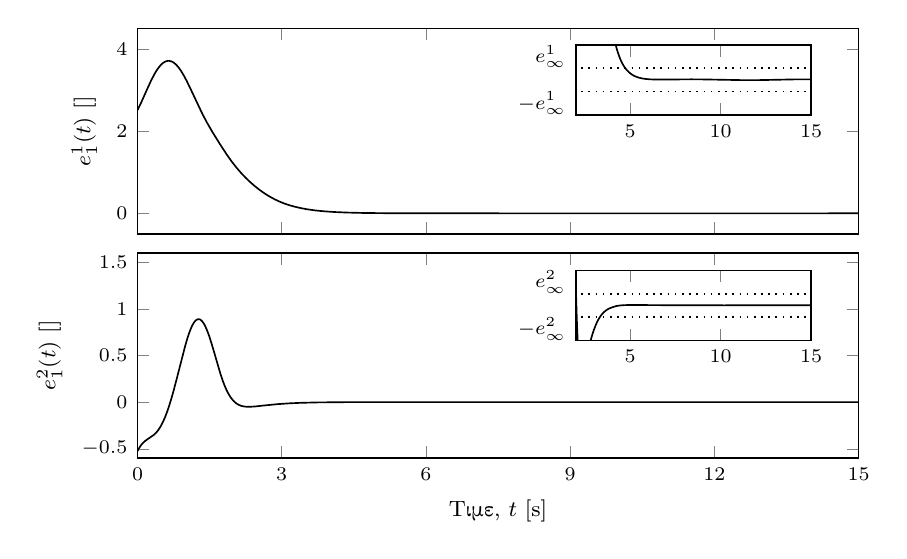
\begin{tikzpicture}

\begin{axis}[%
width=0.944\figurewidth,
height=0.478\figureheight,
at={(0\figurewidth,0.522\figureheight)},
scale only axis,
xmin=0,
xmax=15,
xtick distance=3,
xticklabels={\empty},
ymin=-0.5,
ymax=4.5,
ylabel style={font=\color{white!15!black}},
ylabel={$e_1^1(t)$ [\si{\rad}]},
axis background/.style={fill=white},
xlabel style={font=\footnotesize},ylabel style={font=\footnotesize},ticklabel style={font=\scriptsize},x tick label style={font=\scriptsize},y tick label style={font=\scriptsize},legend style={font=\scriptsize}
]
\addplot [color=black, forget plot]
  table[row sep=crcr]{%
0	2.51327412287183\\
0.0660909396420379	2.67235151771786\\
0.180836592403185	2.97329943568229\\
0.284366058824709	3.23774937183384\\
0.353667900028302	3.39376129719907\\
0.40183260107081	3.48717766993387\\
0.45560552591107	3.57411083663945\\
0.495935219541266	3.62612563799267\\
0.536484488832553	3.66637050799642\\
0.577472909446023	3.69438865666189\\
0.604798523188336	3.70588898947231\\
0.632124136930649	3.71161938650559\\
0.659449750672962	3.71158937104791\\
0.69581662508668	3.70268173646654\\
0.729872726400522	3.68529043396777\\
0.767111872658699	3.65649323307015\\
0.810717108805548	3.61025174639642\\
0.854322344952397	3.55121690371685\\
0.899056388549955	3.47836523206534\\
0.958701780013365	3.36411406750884\\
1.02098832444324	3.22769926327638\\
1.10930584915705	3.01409710316607\\
1.35375535842587	2.40972565747267\\
1.45214476442267	2.19335664473487\\
1.56046829556299	1.97552090918001\\
1.715483223779	1.68344046368741\\
1.86165675878511	1.42186776114133\\
1.95947474771242	1.26090412333102\\
2.05125084352172	1.12303110508366\\
2.14946381145791	0.989115691582157\\
2.24767677939409	0.86783676502162\\
2.35235986184456	0.750953353282545\\
2.44892148720354	0.653466454577629\\
2.54775809132914	0.563287330722769\\
2.65538820849667	0.475614739603921\\
2.74560757734862	0.410247022493493\\
2.85073621103207	0.343023565963238\\
2.95458378770931	0.285580231054603\\
3.05600844763472	0.238299983640893\\
3.17237276165707	0.193425160888507\\
3.28568232022027	0.156994046996717\\
3.40595054907159	0.12518372492805\\
3.54048851604394	0.0966986051464627\\
3.69955699072939	0.0708819425311695\\
3.87149231963165	0.050408843233134\\
4.08981654497144	0.0324991735626305\\
4.34436144777517	0.0193409589695754\\
4.69059070233002	0.00943714389125638\\
5.1950596486038	0.00316877148760319\\
6.12476278067038	0.000370477711042483\\
12.1889903074585	-0.000166362128380726\\
15	0.000366225083421767\\
};
\end{axis}

\begin{axis}[%
width=0.308\figurewidth,
height=0.163\figureheight,
at={(0.574\figurewidth,0.799\figureheight)},
scale only axis,
scaled y ticks = false,
ytick = {-0.0175,0.0175},
ytick style={draw=none},
yticklabels={$-e_\infty^1$, $e_\infty^1$},
xmin=2,
xmax=15,
ymin=-0.02625,
ymax=0.02625,
axis background/.style={fill=white},
xlabel style={font=\footnotesize},ylabel style={font=\footnotesize},ticklabel style={font=\scriptsize},x tick label style={font=\scriptsize},y tick label style={font=\scriptsize},legend style={font=\scriptsize}
]
\addplot [color=black, forget plot]
  table[row sep=crcr]{%
4.18727437574509	0.0266656831612888\\
4.22083478627129	0.0249032341201811\\
4.25439519679749	0.0232543225037247\\
4.28795560732368	0.0217118592776302\\
4.32555950095801	0.0201017862423356\\
4.36316339459233	0.0186082015962921\\
4.40076728822665	0.0172229020816417\\
4.43984349486218	0.0158898866576749\\
4.48039201449891	0.0146129921728235\\
4.52459661680067	0.0133347852848864\\
4.56595994922298	0.0122377375978751\\
4.60732328164529	0.0112287453014837\\
4.64895699198766	0.0102950889548659\\
4.69059070233002	0.00943714389125638\\
4.74028240104325	0.00850393063114652\\
4.78997409975648	0.0076607149707435\\
4.84350869458312	0.00684328947252233\\
4.89896473746647	0.00608610804012244\\
4.96245475579959	0.00531904981443354\\
5.04061420208205	0.00448631203882144\\
5.10226468830174	0.00390796018956507\\
5.16412799516978	0.00339906390042621\\
5.2431240633421	0.00283995560837091\\
5.31522068544955	0.00240656321353505\\
5.38989123433812	0.00202405761604041\\
5.46970963678896	0.00167923300848472\\
5.57613417339007	0.0013058375796291\\
5.68470751324743	0.00100832960357167\\
5.81966485391798	0.00073138907290371\\
5.96650867068311	0.000520079635121462\\
6.12476278067038	0.000370477711042483\\
6.32318392174816	0.000264344944838513\\
6.56958216649834	0.000215594358447646\\
6.92183263344387	0.000233732988874635\\
8.37718925501369	0.000398096518425817\\
8.92845256369849	0.00034255910613723\\
9.59003192506554	0.000193791005997923\\
11.0728828670014	-0.000176677978787509\\
11.6309365872299	-0.000218902810923183\\
12.138258151074	-0.000175184135668971\\
12.7018848548724	-3.93389694561819e-05\\
14.0966139063371	0.000349468479216242\\
14.6248030720684	0.000387514880392459\\
15	0.000366225083421767\\
};
\addplot [color=black, dotted, forget plot]
  table[row sep=crcr]{%
0.699999999999999	0.00874999999999915\\
15	0.00874999999999915\\
};
\addplot [color=black, dotted, forget plot]
  table[row sep=crcr]{%
0.699999999999999	-0.00874999999999915\\
15	-0.00874999999999915\\
};
\end{axis}

\begin{axis}[%
width=0.944\figurewidth,
height=0.478\figureheight,
at={(0\figurewidth,0\figureheight)},
scale only axis,
xmin=0,
xmax=15,
xtick distance = 3,
xlabel style={font=\color{white!15!black}},
xlabel={Time, $t$ [\si{\second}]},
ymin=-0.6,
ymax=1.6,
ylabel style={font=\color{white!15!black}},
ylabel={$e_1^2(t)$ [\si{\rad}]},
axis background/.style={fill=white},
xlabel style={font=\footnotesize},ylabel style={font=\footnotesize},ticklabel style={font=\scriptsize},x tick label style={font=\scriptsize},y tick label style={font=\scriptsize},legend style={font=\scriptsize}
]
\addplot [color=black, forget plot]
  table[row sep=crcr]{%
0	-0.523598775598298\\
0.0282482984885686	-0.496335470077891\\
0.0585224114113441	-0.471601398020104\\
0.0857288129488385	-0.452895002667601\\
0.11518562290904	-0.435877954334291\\
0.146326770262677	-0.420900697707905\\
0.192339866450022	-0.402863716178924\\
0.342094076750822	-0.349661738165191\\
0.376815546583265	-0.332761319971047\\
0.415275832280875	-0.310049012024532\\
0.45560552591107	-0.280929596057339\\
0.495935219541266	-0.245756816879545\\
0.536484488832553	-0.203886788491156\\
0.577472909446023	-0.154754074508045\\
0.618461330059493	-0.0988168181974647\\
0.659449750672962	-0.0363317629363422\\
0.707168658857961	0.0440252923140108\\
0.752576793943083	0.127114341415979\\
0.810717108805548	0.240757742826867\\
0.989845052228302	0.599600220122923\\
1.03655996055071	0.681844929975618\\
1.07293290485388	0.738704041312317\\
1.10930584915705	0.78782498487759\\
1.1335544786925	0.815704917323361\\
1.15780310822795	0.839361752496993\\
1.18230012228336	0.858746969795371\\
1.20427461325725	0.872135424735658\\
1.22372658114963	0.880759244309242\\
1.24956865309951	0.887469870781544\\
1.27182638374009	0.888895496530772\\
1.29324351991665	0.886484519226972\\
1.31143260866958	0.881559524613728\\
1.33362423136743	0.872039924875265\\
1.35375535842587	0.860150477250547\\
1.37388648548431	0.845267878489405\\
1.39401761254276	0.827509930557492\\
1.41726847329472	0.803601020757174\\
1.45214476442267	0.761423341235933\\
1.48976431658434	0.708425768210997\\
1.52666712302163	0.650197722445199\\
1.57173535307678	0.572943293408256\\
1.73039552368339	0.293668615799666\\
1.77398139498391	0.227559553443649\\
1.8128070465224	0.175374094325923\\
1.84522292600311	0.136857049061174\\
1.87809059156711	0.102437614630009\\
1.9086096501216	0.0744951687071111\\
1.93912870867609	0.0502124607672361\\
1.96964776723058	0.0293531367392923\\
2.00022937439817	0.0116280113453389\\
2.04104654969701	-0.00754328537264826\\
2.07580408550577	-0.0202765860050036\\
2.11263394848184	-0.0306469206267277\\
2.16174043244993	-0.0402879127308413\\
2.21084691641802	-0.0461189750105948\\
2.27316500464543	-0.0495034256080764\\
2.34673139848177	-0.0496685326678143\\
2.44892148720354	-0.0461345095455705\\
2.66827668976124	-0.0339764874830344\\
2.92211398817853	-0.0211467039702189\\
3.15753055070054	-0.0127985909640405\\
3.40595054907159	-0.00713953250301991\\
3.74358683966652	-0.00301009050917322\\
4.28795560732368	-0.000333960514902643\\
5.2431240633421	0.00031472420077705\\
15	6.38197133024931e-05\\
};
\end{axis}

\begin{axis}[%
width=0.308\figurewidth,
height=0.163\figureheight,
at={(0.574\figurewidth,0.274\figureheight)},
scale only axis,
unbounded coords=jump,
scaled y ticks = false,
ytick = {-0.0175,0.0175},
ytick style={draw=none},
yticklabels={$-e_\infty^2$, $e_\infty^2$},
xmin=2,
xmax=15,
ymin=-0.02625,
ymax=0.02625,
axis background/.style={fill=white},
xlabel style={font=\footnotesize},ylabel style={font=\footnotesize},ticklabel style={font=\scriptsize},x tick label style={font=\scriptsize},y tick label style={font=\scriptsize},legend style={font=\scriptsize}
]
\addplot [color=black, forget plot]
  table[row sep=crcr]{%
1.99002508057346	0.0172053511643337\\
2.00022937439817	0.0116280113453389\\
2.01043366822288	0.00637476410078364\\
2.02063796204759	0.00143535727620758\\
2.0308422558723	-0.00320053329074987\\
2.04104654969701	-0.00754328537264826\\
2.05125084352172	-0.0116033116824479\\
2.06352746451375	-0.0161279379257735\\
2.07580408550577	-0.0202765860050036\\
2.08808070649779	-0.0240673440732504\\
2.10035732748982	-0.0275181868124506\\
nan	nan\\
2.79990319670516	-0.026868054045341\\
2.8337918729231	-0.0251880637898729\\
2.86768054914104	-0.0235788145442228\\
2.90587908841315	-0.0218521961452964\\
2.93834888794392	-0.0204581632285024\\
2.9708186874747	-0.0191318000884202\\
3.00567721208393	-0.0178000675296595\\
3.0312787620873	-0.0169095284941339\\
3.07575697872721	-0.0153573494560835\\
3.11037958800308	-0.0142259080383749\\
3.14543629862737	-0.0131525515825714\\
3.17979386713534	-0.0121682551889517\\
3.21400363166301	-0.01125163306952\\
3.24984297594164	-0.0103558861761179\\
3.28568232022027	-0.00952271669859606\\
3.33460493739823	-0.00848014733249514\\
3.3835275545762	-0.00753915210030698\\
3.42837354356698	-0.00675874329101767\\
3.47321953255776	-0.00605067386865699\\
3.51806552154855	-0.00540917118253503\\
3.56321258385614	-0.00482507698949419\\
3.60866071948056	-0.00429434386648353\\
3.67683292291718	-0.00359514205460876\\
3.74358683966652	-0.00301009050917322\\
3.80750418304128	-0.00253020422752925\\
3.87149231963165	-0.00211818504611117\\
3.95699861699376	-0.00165896821818556\\
4.17049417048199	-0.000680944143297779\\
4.25439519679749	-0.000420566209619722\\
4.36316339459233	-0.000170355039424308\\
4.48039201449891	1.63388845049184e-05\\
4.62120118509275	0.000160050312578264\\
4.80653799932755	0.00026184484732461\\
5.06646115748065	0.000311686146524437\\
5.49631577093924	0.000301703601653713\\
6.37585526406244	0.000200632495726438\\
7.15697085477277	0.000150234919209069\\
10.1756385548839	5.9263264136078e-05\\
13.8356250037231	0.000119259342195477\\
15	6.38197133024931e-05\\
};
\addplot [color=black, dotted, forget plot]
  table[row sep=crcr]{%
0.699999999999999	0.00874999999999915\\
15	0.00874999999999915\\
};
\addplot [color=black, dotted, forget plot]
  table[row sep=crcr]{%
0.699999999999999	-0.00874999999999915\\
15	-0.00874999999999915\\
};
\end{axis}
\end{tikzpicture}%
    \end{frame}
    
    \begin{frame}
        \frametitle{Ρομποτικός βραχίονας}
        \selectlanguage{english}
        % This file was created by matlab2tikz.
%
\tikzstyle{every node}=[font=\footnotesize]
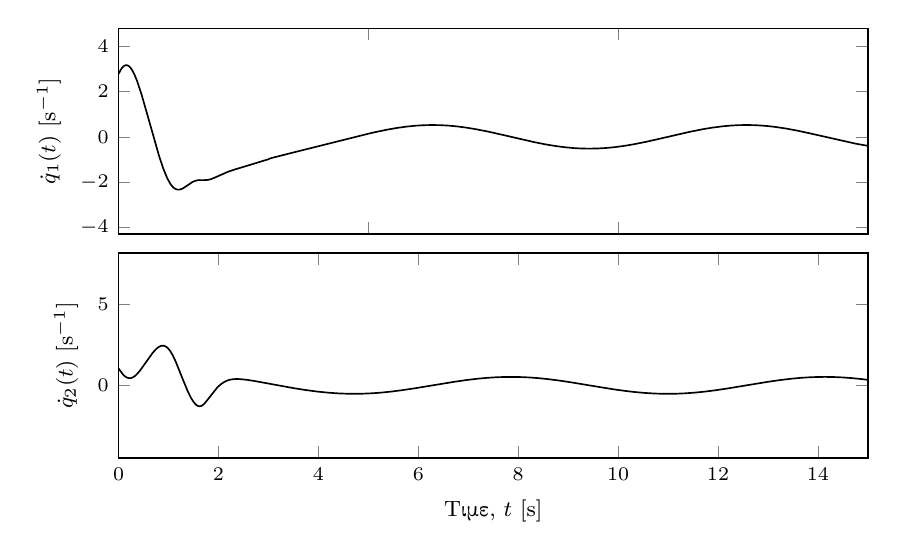
\begin{tikzpicture}

\begin{axis}[%
width=0.981\figurewidth,
height=0.478\figureheight,
at={(0\figurewidth,0.522\figureheight)},
scale only axis,
xmin=0,
xmax=15,
xtick={0,5,10,15},
xticklabels={\empty},
ymin=-4.3,
ymax=4.8,
ylabel style={font=\color{white!15!black}},
ylabel={$\dot q_1(t)$ [\si{\rad\per\second}]},
axis background/.style={fill=white},
xlabel style={font=\footnotesize},ylabel style={font=\footnotesize},ticklabel style={font=\scriptsize},x tick label style={font=\scriptsize},y tick label style={font=\scriptsize},legend style={font=\scriptsize}
]
\addplot [color=black, forget plot]
  table[row sep=crcr]{%
0	2.79252680319093\\
0.0509538831806502	2.99998495027441\\
0.0857288129488385	3.09764644484296\\
0.11518562290904	3.15038268482849\\
0.134823496215841	3.16977197991961\\
0.157830044309513	3.17622822013983\\
0.180836592403185	3.16513082772653\\
0.203843140496858	3.1366677426144\\
0.238352962637364	3.06231737765453\\
0.272862784777873	2.95191304967182\\
0.318946430195862	2.75338785096634\\
0.376815546583265	2.43362172364231\\
0.45560552591107	1.90388517949963\\
0.577472909446023	0.964990321860586\\
0.810717108805548	-0.849641184978744\\
0.899056388549955	-1.43280338426337\\
0.974273416120834	-1.83599675849152\\
1.03655996055071	-2.08592006276174\\
1.0850572196216	-2.22164966244682\\
1.12143016392477	-2.28920419175627\\
1.15780310822795	-2.32874074097425\\
1.18230012228336	-2.34071434421318\\
1.21400059720344	-2.34042002877061\\
1.24956865309951	-2.3215979889061\\
1.29324351991665	-2.27706603403765\\
1.35375535842587	-2.18987341786271\\
1.47539562517463	-2.0067800493303\\
1.52666712302163	-1.95537076258327\\
1.57173535307678	-1.92865430060227\\
1.61992958491004	-1.91678076788751\\
1.68565862397022	-1.91745079852081\\
1.75676140099601	-1.91631908450134\\
1.80504191621471	-1.90120830485258\\
1.85343984239411	-1.8712726681155\\
1.91878266963976	-1.81287970107659\\
2.18629367443398	-1.55181083181825\\
2.32688156999146	-1.44595807629359\\
2.58682140166169	-1.27318911226015\\
3.00141448913614	-0.99239597795621\\
3.02137392429866	-0.966020173728669\\
3.07575697872721	-0.930935231714596\\
3.51806552154855	-0.681868881720765\\
4.48039201449891	-0.150609600073405\\
5.00000000009076	0.138064163312604\\
5.13319634173576	0.205668355245482\\
5.36328510018784	0.312250102661672\\
5.57613417339007	0.39498172578319\\
5.76788536604122	0.453639600353622\\
5.94778797765301	0.493185917704132\\
6.11019018722018	0.515010375985931\\
6.27051257943388	0.523112891928983\\
6.42852660637672	0.517865705203803\\
6.59899072533461	0.497664953012729\\
6.77544207835218	0.461506672265223\\
6.94991540802872	0.411611877824454\\
7.15697085477277	0.336290887402432\\
7.39896695805906	0.230284389413471\\
7.69852329881502	0.0812023228519969\\
8.333356538999	-0.24151754868924\\
8.55252011907245	-0.336802817304326\\
8.74048634138547	-0.405842222408211\\
8.92845256369849	-0.46058588761022\\
9.11826525916181	-0.499398444885598\\
9.26200963562203	-0.516906934793932\\
9.41588739621301	-0.523829303409123\\
9.59003192506554	-0.516735848266171\\
9.76417645391807	-0.494012242363036\\
9.9383209827706	-0.456345991769661\\
10.1281750404612	-0.399605215652949\\
10.3199552802739	-0.327719298085212\\
10.5669037629971	-0.217883568887313\\
10.8699542414638	-0.0657945983164403\\
11.4280079616923	0.219374797440809\\
11.6816687436143	0.331731772614003\\
11.884597369152	0.406637995645863\\
12.0875259946896	0.464859198509995\\
12.2397224638429	0.496108809704509\\
12.3933121788886	0.516015577136645\\
12.5475985168805	0.523780134013528\\
12.7018848548724	0.519099877198265\\
12.8561711928644	0.502085366398315\\
13.0104575308563	0.473140437586276\\
13.1647438688483	0.432952671454167\\
13.3704589861708	0.363566512625315\\
13.5761741034934	0.278846470616013\\
13.8356250037231	0.155724631239684\\
14.7559207417799	-0.30373969643065\\
14.9706028980085	-0.387691065690605\\
15	-0.397878433854268\\
};
\end{axis}

\begin{axis}[%
width=0.981\figurewidth,
height=0.478\figureheight,
at={(0\figurewidth,0\figureheight)},
scale only axis,
xmin=0,
xmax=15,
xlabel style={font=\color{white!15!black}},
xlabel={Time, $t$ [\si{\second}]},
ymin=-4.5,
ymax=8.2,
ylabel style={font=\color{white!15!black}},
ylabel={$\dot q_2(t)$ [\si{\rad\per\second}]},
axis background/.style={fill=white},
xlabel style={font=\footnotesize},ylabel style={font=\footnotesize},ticklabel style={font=\scriptsize},x tick label style={font=\scriptsize},y tick label style={font=\scriptsize},legend style={font=\scriptsize}
]
\addplot [color=black, forget plot]
  table[row sep=crcr]{%
0	1.0471975511966\\
0.000178558049340083	1.03948493757308\\
0.0955477496022397	0.644565838145704\\
0.134823496215841	0.539025400647574\\
0.169333318356349	0.477946101850241\\
0.203843140496858	0.447617497716879\\
0.226849688590528	0.444542862933076\\
0.249856236684201	0.454920629669743\\
0.284366058824709	0.494669097592528\\
0.318946430195862	0.561507144089269\\
0.365241723305784	0.687955042592035\\
0.42871906349094	0.915353969795532\\
0.522821681961396	1.32066326109971\\
0.6844645913154	2.01991846770099\\
0.752576793943083	2.24961465240898\\
0.796182030089932	2.3584873256979\\
0.839787266236781	2.42906250445439\\
0.86923369281825	2.45149799556336\\
0.899056388549955	2.45109552905349\\
0.928879084281661	2.42560987919158\\
0.958701780013365	2.37360958070174\\
0.989845052228302	2.29004294157232\\
1.03655996055071	2.1084792479031\\
1.0850572196216	1.85264063681194\\
1.14567879346022	1.45297005485379\\
1.25762669710135	0.587096422592751\\
1.38395204901354	-0.367910282545298\\
1.45214476442267	-0.79071215831449\\
1.50413300799405	-1.04056679013023\\
1.54920123804921	-1.19358615197087\\
1.58300241059057	-1.26392345102228\\
1.61069779133017	-1.29058651087655\\
1.62916137848991	-1.29217281201627\\
1.64762496564964	-1.28066584702144\\
1.67668430401458	-1.236743996532\\
1.70802707382681	-1.15734818974679\\
1.75676140099601	-0.984907848192501\\
1.97982078674875	-0.115624877209209\\
2.05125084352172	0.0799578497893929\\
2.11263394848184	0.206386394067101\\
2.17401705344196	0.295806911228929\\
2.22312353741005	0.343421225388363\\
2.27316500464543	0.373465781843977\\
2.32984600839343	0.389505893947717\\
2.39476619385409	0.390530922545505\\
2.46904885799141	0.376289802279166\\
2.57380029821751	0.339104847233134\\
2.71983061481949	0.269173526737923\\
2.95458378770931	0.138196207810539\\
3.49564252705316	-0.167231839141873\\
3.74358683966652	-0.288414007750843\\
3.95699861699376	-0.376357214855174\\
4.00000000006521	-0.391925706431827\\
4.04552672055266	-0.406321166488826\\
4.22083478627129	-0.458588060399101\\
4.40076728822665	-0.496682196973396\\
4.57974772669709	-0.518089239665189\\
4.74028240104325	-0.522912606227521\\
4.89896473746647	-0.514286904443884\\
5.07507680928019	-0.48947624328823\\
5.2431240633421	-0.451591838947365\\
5.44310350263868	-0.389987783420189\\
5.65756417828309	-0.306695201317311\\
5.9103465915928	-0.19079246745434\\
5.99999999999181	-0.146362202623269\\
6.19763768005213	-0.0449045830919452\\
6.74603351951591	0.233727215045869\\
6.97799818261357	0.335184230378143\\
7.19469332916636	0.413824195166503\\
7.39896695805906	0.470278683858607\\
7.5803983579208	0.504074337502045\\
7.75683210333399	0.521073620405568\\
7.93735508951264	0.52171988054846\\
8.10090136499366	0.507656158675003\\
8.24569110696962	0.48387886261194\\
8.42102197102838	0.441594382379316\\
8.59951167465071	0.384650704196611\\
8.83446945254198	0.291403695468004\\
9.0703504670084	0.181691060569092\\
9.47393557249719	-0.0257277869452697\\
9.88027280648642	-0.230314348023237\\
10.1281750404612	-0.338644105619037\\
10.3199552802739	-0.408547569842534\\
10.5175140664524	-0.464871901872058\\
10.7177577723105	-0.503499364486975\\
10.8699542414638	-0.519452567124322\\
11.022150710617	-0.523395795513983\\
11.1743471797702	-0.515237568495728\\
11.3265436489235	-0.495166292028765\\
11.5294722744611	-0.450713496492806\\
11.7324008999988	-0.387761721111302\\
11.9353295255364	-0.308894865611123\\
12.1889903074585	-0.192914169065842\\
12.5475985168805	-0.00980096986871182\\
13.0104575308563	0.224974600569226\\
13.2676014275096	0.337811366688115\\
13.4733165448321	0.412394563755157\\
13.6790316621547	0.469585777704213\\
13.8356250037231	0.499944801812456\\
13.9922183452915	0.518069727969479\\
14.1488116868599	0.523517461615056\\
14.3209075871988	0.514733495594864\\
14.4936854023568	0.4906193268328\\
14.6685089619722	0.451355424238626\\
14.8687168326026	0.389581823457952\\
15	0.340446141949046\\
};
\end{axis}
\end{tikzpicture}%
    \end{frame}
    
    \begin{frame}
        \frametitle{Ρομποτικός βραχίονας}
        \selectlanguage{english}
        % This file was created by matlab2tikz.
%
\tikzstyle{every node}=[font=\footnotesize]
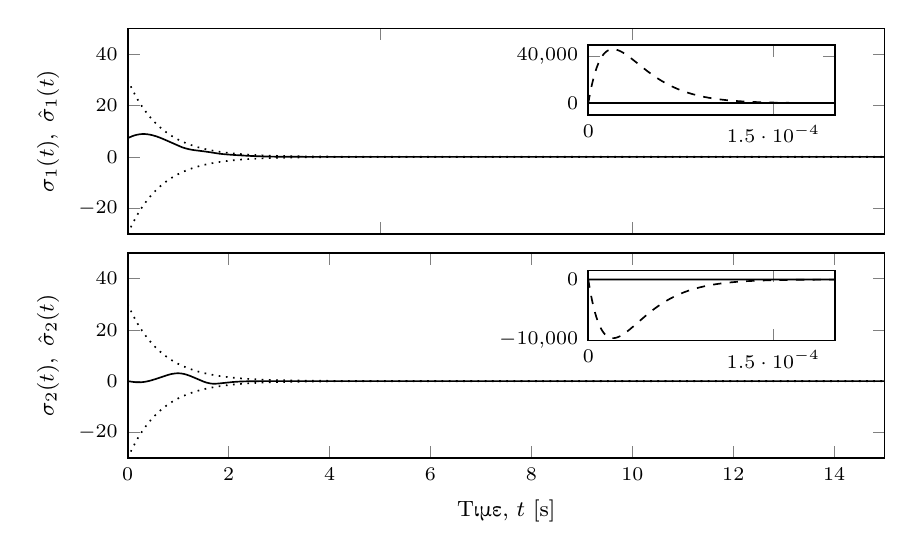
\begin{tikzpicture}

\begin{axis}[%
width=0.991\figurewidth,
height=0.478\figureheight,
at={(0\figurewidth,0.522\figureheight)},
scale only axis,
xmin=0,
xmax=15,
xtick={0,5,10,15},
xticklabels={\empty},
ymin=-30,
ymax=50,
ylabel style={font=\color{white!15!black}},
ylabel={$\sigma_1(t),\ \hat \sigma_1(t)$},
axis background/.style={fill=white},
xlabel style={font=\footnotesize},ylabel style={font=\footnotesize},ticklabel style={font=\scriptsize},x tick label style={font=\scriptsize},y tick label style={font=\scriptsize},legend style={font=\scriptsize}
]
\addplot [color=black, forget plot]
  table[row sep=crcr]{%
0	7.2954762733363\\
0.0857288129488385	8.02087764343114\\
0.146326770262677	8.4204175141355\\
0.192339866450022	8.64655672336024\\
0.238352962637364	8.80040465064285\\
0.272862784777873	8.86735569321313\\
0.295869332871545	8.88914387215856\\
0.318946430195862	8.89305288580403\\
0.342094076750822	8.87943783027045\\
0.365241723305784	8.84889561107417\\
0.40183260107081	8.76786748151283\\
0.442162294701005	8.63540577200902\\
0.495935219541266	8.39569396533899\\
0.563810102574866	8.00434357374873\\
0.645786943801806	7.42349079020822\\
0.741224760171802	6.63442237017222\\
1.07293290485388	3.76557195919163\\
1.14567879346022	3.31029751943399\\
1.21400059720344	2.97496798850647\\
1.28103884769544	2.72370240456643\\
1.34368979489665	2.54246975136395\\
1.44051933404669	2.31440020086987\\
1.53793418053542	2.07468862385194\\
1.62916137848991	1.80316514417517\\
1.80504191621471	1.26206699391619\\
1.87809059156711	1.09495855843381\\
1.95947474771242	0.949304390299764\\
2.06352746451375	0.795897124616474\\
2.21084691641802	0.604601966628426\\
2.35798832520734	0.436450559590371\\
2.47911254338535	0.318886273406219\\
2.58682140166169	0.232325911125214\\
2.69405365229036	0.163255414992321\\
2.79990319670516	0.110947283228159\\
2.92211398817853	0.0677762014013439\\
3.00249585321438	0.052524058932109\\
3.0221254245068	0.0603960174561742\\
3.08144965594007	0.0506139432148451\\
3.23789652784876	0.0265119296199128\\
3.45079653806237	0.00993994539616416\\
3.78619840191636	0.00102807882973011\\
4.60732328164529	-0.000928255271576361\\
15	0.000625677322281248\\
};
\addplot [color=black, dotted, forget plot]
  table[row sep=crcr]{%
0	30\\
0.0955477496022397	25.9989336967413\\
0.19233986645002	22.4901555619394\\
0.295869332871543	19.2602791338603\\
0.401832601070812	16.4349966785703\\
0.495935219541266	14.2760295694871\\
0.591135716317179	12.3809300658203\\
0.695816625086682	10.5868911130505\\
0.79618203008993	9.11212024591008\\
0.899056388549955	7.81413734615192\\
1.00541668833577	6.6669906062661\\
1.10930584915705	5.7100039543817\\
1.21400059720344	4.88524460697276\\
1.31749563825389	4.1878156602318\\
1.41726847329472	3.61057972546333\\
1.51540006550784	3.12116720927892\\
1.61992958491004	2.67330233805938\\
1.7229393737312	2.29557899582052\\
1.8287890932211	1.96370037271144\\
1.92895568915793	1.69463301092852\\
2.0308422558723	1.45942275878951\\
2.13718719046589	1.24939893199893\\
2.24767677939409	1.06392530550929\\
2.36361678857012	0.899680547988748\\
2.47911254338534	0.762138157870087\\
2.59984250510587	0.641692185927369\\
2.71983061481949	0.541760948619725\\
2.85073621103207	0.451414432508955\\
2.99916484749627	0.368298352280256\\
3.15010944522227	0.300767308286254\\
3.31829739833891	0.241508012971419\\
3.49564252705315	0.193273020923154\\
3.72228105854159	0.147658793599618\\
3.98490691920805	0.110976564742309\\
4.30675755414084	0.0818827114494169\\
4.72371850147217	0.0600834323054187\\
5.2911884780804	0.0457081228226812\\
6.24622094630663	0.0375560264724157\\
8.78747789696373	0.0350565046958131\\
15	0.0350000050697723\\
};
\addplot [color=black, dotted, forget plot]
  table[row sep=crcr]{%
0	-30\\
0.0955477496022397	-25.9989336967413\\
0.19233986645002	-22.4901555619394\\
0.295869332871543	-19.2602791338603\\
0.401832601070812	-16.4349966785703\\
0.495935219541266	-14.2760295694871\\
0.591135716317179	-12.3809300658203\\
0.695816625086682	-10.5868911130505\\
0.79618203008993	-9.11212024591008\\
0.899056388549955	-7.81413734615192\\
1.00541668833577	-6.6669906062661\\
1.10930584915705	-5.7100039543817\\
1.21400059720344	-4.88524460697276\\
1.31749563825389	-4.1878156602318\\
1.41726847329472	-3.61057972546333\\
1.51540006550784	-3.12116720927892\\
1.61992958491004	-2.67330233805938\\
1.7229393737312	-2.29557899582052\\
1.8287890932211	-1.96370037271144\\
1.92895568915793	-1.69463301092852\\
2.0308422558723	-1.45942275878951\\
2.13718719046589	-1.24939893199893\\
2.24767677939409	-1.06392530550929\\
2.36361678857012	-0.899680547988748\\
2.47911254338534	-0.762138157870087\\
2.59984250510587	-0.641692185927369\\
2.71983061481949	-0.541760948619725\\
2.85073621103207	-0.451414432508955\\
2.99916484749627	-0.368298352280256\\
3.15010944522227	-0.300767308286254\\
3.31829739833891	-0.241508012971419\\
3.49564252705315	-0.193273020923154\\
3.72228105854159	-0.147658793599618\\
3.98490691920805	-0.110976564742309\\
4.30675755414084	-0.0818827114494169\\
4.72371850147217	-0.0600834323054187\\
5.2911884780804	-0.0457081228226812\\
6.24622094630663	-0.0375560264724157\\
8.78747789696373	-0.0350565046958131\\
15	-0.0350000050697723\\
};
\end{axis}

\begin{axis}[%
width=0.323\figurewidth,
height=0.163\figureheight,
at={(0.603\figurewidth,0.799\figureheight)},
scale only axis,
xmin=0,
xmax=0.0002,
ymin=-10000,
ymax=50000,
scaled y ticks = false,
scaled x ticks = false,
xtick = {0,0.00015},
ytick = {0,40000},
axis background/.style={fill=white},
xlabel style={font=\footnotesize},ylabel style={font=\footnotesize},ticklabel style={font=\scriptsize},x tick label style={font=\scriptsize},y tick label style={font=\scriptsize},legend style={font=\scriptsize}
]
\addplot [color=black, forget plot]
  table[row sep=crcr]{%
0	7.2954762733363\\
2.85463155336174e-08	7.2954760864713\\
3.90358380286671e-07	7.29548077918415\\
0.000178558049340083	7.29780384515835\\
0.000178670583830254	7.29780055545965\\
0.000180402780324052	7.29774945092869\\
0.000181198375756253	7.29773568596859\\
0.000182126744739719	7.29772299824263\\
0.000183820320846628	7.29770315074565\\
0.000186217804525768	7.29767783581035\\
0.000189671676380954	7.29764353561953\\
0.000195025095092838	7.2975923884729\\
0.000200054489301493	7.29754534173188\\
};
\addplot [color=black, dashed, forget plot]
  table[row sep=crcr]{%
0	0\\
1.33952562464401e-06	7871.88392766791\\
2.85554415313527e-06	15555.9968291478\\
4.34539833804592e-06	21972.933824098\\
5.33863203600049e-06	25687.4851118208\\
6.68650318402797e-06	30076.1927577757\\
8.03437433205545e-06	33783.7765707259\\
9.38223820412531e-06	36880.3777483795\\
1.00561737781391e-05	38219.7553157803\\
1.10827459138818e-05	40013.9709929829\\
1.21093107736669e-05	41532.9857069545\\
1.31358829094097e-05	42799.8468570355\\
1.41624550451525e-05	43835.9842996798\\
1.51890199049376e-05	44661.3143580437\\
1.62155920406803e-05	45294.3379121399\\
1.72421569004655e-05	45752.2323813246\\
1.83411248144694e-05	46066.3859638995\\
1.94400927284732e-05	46216.1794984327\\
2.05390606424771e-05	46218.2904705136\\
2.1638028556481e-05	46088.0826856197\\
2.27369964704849e-05	45839.6991195777\\
2.38359643844888e-05	45486.1487042815\\
2.4934925022535e-05	45039.3871956523\\
2.6116453227587e-05	44467.616883255\\
2.72979814326391e-05	43813.2555739182\\
2.84795096376911e-05	43087.6607434613\\
3.08425660477951e-05	41463.124332917\\
3.32056224578992e-05	39665.6566597817\\
3.6977136915084e-05	36580.2955582615\\
4.73194013466127e-05	27912.8074306452\\
5.13045961270109e-05	24796.9495605165\\
5.41036133654416e-05	22735.2895046998\\
5.69026233279146e-05	20789.3163911429\\
5.97016405663453e-05	18963.9768283091\\
6.2574639741797e-05	17217.5934679845\\
6.55216208542697e-05	15559.1463574191\\
6.84686092427e-05	14032.0833795475\\
7.14155903551728e-05	12631.5339664408\\
7.452455611201e-05	11284.5018614975\\
7.76335218688473e-05	10063.6684377934\\
8.07424876256846e-05	8960.61623865582\\
8.39456915855408e-05	7938.22132731228\\
8.72431483003311e-05	6996.91791906664\\
9.05406050151214e-05	6158.53561504811\\
9.38380544539541e-05	5413.53406544297\\
9.56066287471913e-05	5049.26474485271\\
9.73752103163861e-05	4707.93057461482\\
9.91437846096233e-05	4388.25858848526\\
0.00010091235890286	4089.02698752803\\
0.000102680933196098	3809.06560455517\\
0.000104449507489335	3547.25594375029\\
0.000106218081782572	3302.53082027198\\
0.000108312720840331	3033.39403459673\\
0.00011040735989809	2785.19935695579\\
0.000112121691927314	2596.59659415113\\
0.000113836031232495	2420.23458387947\\
0.000115550363261718	2255.37491001724\\
0.000117264702566899	2101.3179015508\\
0.00011897904187208	1957.40124446259\\
0.000120693373901304	1822.99854301882\\
0.000122760684462264	1672.73809661239\\
0.000124827995023225	1534.47949756471\\
0.000126895305584185	1407.31454951827\\
0.000128962616145145	1290.3976843343\\
0.000131029926706105	1182.942469538\\
0.000133097237267066	1084.21812601308\\
0.000135164547828026	993.546145975386\\
0.000137515387905296	899.425445147521\\
0.000139866227982566	814.051146625839\\
0.000142217060783878	736.640854112076\\
0.000144567900861148	666.478144931563\\
0.000146918740938418	602.907552224569\\
0.000149269581015687	545.329852536503\\
0.000151620421092957	493.197654816395\\
0.000153578032040969	453.579622960962\\
0.000155535650264937	417.125254194681\\
0.000157493261212949	383.58902894373\\
0.00015945087216096	352.743701483334\\
0.000161408483108971	324.379026620853\\
0.00016336610133294	298.300571889085\\
0.000165323712280951	274.328599649416\\
0.000167281323228963	252.297014844327\\
0.000169238934176974	232.052381142414\\
0.000171196552400943	213.453004726151\\
0.000173154163348954	196.368079878317\\
0.000175111774296965	180.676890672607\\
0.000177765643456951	161.432790571576\\
0.000180228700628504	145.461117662802\\
0.000182126743311528	134.275410789058\\
0.000184419688594062	121.946761453393\\
0.000186217803275213	113.110702108039\\
0.000188808211532887	101.54934404065\\
0.000191398612514604	91.2354012642681\\
0.000193816267710645	82.6176270416108\\
0.000196233922906686	74.8741121747589\\
0.000198651578102726	67.9174927223066\\
0.000200054491870105	64.2101077731932\\
};
\end{axis}

\begin{axis}[%
width=0.991\figurewidth,
height=0.478\figureheight,
at={(0\figurewidth,0\figureheight)},
scale only axis,
xmin=0,
xmax=15,
xlabel style={font=\color{white!15!black}},
xlabel={Time, $t$ [\si{\second}]},
ymin=-30,
ymax=50,
ylabel style={font=\color{white!15!black}},
ylabel={$\sigma_2(t),\ \hat \sigma_2(t)$},
axis background/.style={fill=white},
xlabel style={font=\footnotesize},ylabel style={font=\footnotesize},ticklabel style={font=\scriptsize},x tick label style={font=\scriptsize},y tick label style={font=\scriptsize},legend style={font=\scriptsize}
]
\addplot [color=black, forget plot]
  table[row sep=crcr]{%
0	0\\
0.000178558049340083	-0.00743352893554672\\
0.125004559562441	-0.365091354729026\\
0.157830044309513	-0.419387738310695\\
0.192339866450022	-0.451530252160664\\
0.215346414543692	-0.45748950411933\\
0.238352962637364	-0.450468770945829\\
0.261359510731037	-0.430194326657332\\
0.295869332871545	-0.374856775749786\\
0.330520253473342	-0.289834684729122\\
0.376815546583265	-0.132891486235643\\
0.42871906349094	0.0957290803900577\\
0.495935219541266	0.459440584677711\\
0.591135716317179	1.06384769601581\\
0.796182030089932	2.40776574005366\\
0.854322344952397	2.70664668297112\\
0.899056388549955	2.88323065017243\\
0.943790432147514	3.00124271202936\\
0.974273416120834	3.04313961869816\\
0.989845052228302	3.05154572377195\\
1.00541668833577	3.05084354154297\\
1.02098832444324	3.0408690059552\\
1.04868427531843	2.99997519675559\\
1.0850572196216	2.9016022304574\\
1.12143016392477	2.75478215236734\\
1.17005161525565	2.49088648992833\\
1.23345256509581	2.0535471224044\\
1.3235586678382	1.31650880768149\\
1.50413300799405	-0.190186834166722\\
1.57173535307678	-0.622679504226145\\
1.61992958491004	-0.843559233271531\\
1.6587356641033	-0.956939220158187\\
1.68565862397022	-1.0002219056496\\
1.70802707382681	-1.0153393376067\\
1.73039552368339	-1.01369323769445\\
1.75676140099601	-0.993940867096923\\
1.79727678590701	-0.936478459584745\\
1.86165675878511	-0.808823076243\\
2.06352746451375	-0.385253331410611\\
2.13718719046589	-0.267433292517333\\
2.198570295426	-0.191628042140323\\
2.25995340038612	-0.135133405375129\\
2.33547447175621	-0.0872660514966057\\
2.42028713577528	-0.0534157964947077\\
2.51541263989186	-0.0305419037556494\\
2.65538820849667	-0.0122670161930589\\
2.86768054914104	-0.000737852712212828\\
3.26178942403451	0.00338478221635086\\
15	8.38644829226354e-05\\
};
\addplot [color=black, dotted, forget plot]
  table[row sep=crcr]{%
0	30\\
0.0955477496022397	25.9989336967413\\
0.19233986645002	22.4901555619394\\
0.295869332871543	19.2602791338603\\
0.401832601070812	16.4349966785703\\
0.495935219541266	14.2760295694871\\
0.591135716317179	12.3809300658203\\
0.695816625086682	10.5868911130505\\
0.79618203008993	9.11212024591008\\
0.899056388549955	7.81413734615192\\
1.00541668833577	6.6669906062661\\
1.10930584915705	5.7100039543817\\
1.21400059720344	4.88524460697276\\
1.31749563825389	4.1878156602318\\
1.41726847329472	3.61057972546333\\
1.51540006550784	3.12116720927892\\
1.61992958491004	2.67330233805938\\
1.7229393737312	2.29557899582052\\
1.8287890932211	1.96370037271144\\
1.92895568915793	1.69463301092852\\
2.0308422558723	1.45942275878951\\
2.13718719046589	1.24939893199893\\
2.24767677939409	1.06392530550929\\
2.36361678857012	0.899680547988748\\
2.47911254338534	0.762138157870087\\
2.59984250510587	0.641692185927369\\
2.71983061481949	0.541760948619725\\
2.85073621103207	0.451414432508955\\
2.99916484749627	0.368298352280256\\
3.15010944522227	0.300767308286254\\
3.31829739833891	0.241508012971419\\
3.49564252705315	0.193273020923154\\
3.72228105854159	0.147658793599618\\
3.98490691920805	0.110976564742309\\
4.30675755414084	0.0818827114494169\\
4.72371850147217	0.0600834323054187\\
5.2911884780804	0.0457081228226812\\
6.24622094630663	0.0375560264724157\\
8.78747789696373	0.0350565046958131\\
15	0.0350000050697723\\
};
\addplot [color=black, dotted, forget plot]
  table[row sep=crcr]{%
0	-30\\
0.0955477496022397	-25.9989336967413\\
0.19233986645002	-22.4901555619394\\
0.295869332871543	-19.2602791338603\\
0.401832601070812	-16.4349966785703\\
0.495935219541266	-14.2760295694871\\
0.591135716317179	-12.3809300658203\\
0.695816625086682	-10.5868911130505\\
0.79618203008993	-9.11212024591008\\
0.899056388549955	-7.81413734615192\\
1.00541668833577	-6.6669906062661\\
1.10930584915705	-5.7100039543817\\
1.21400059720344	-4.88524460697276\\
1.31749563825389	-4.1878156602318\\
1.41726847329472	-3.61057972546333\\
1.51540006550784	-3.12116720927892\\
1.61992958491004	-2.67330233805938\\
1.7229393737312	-2.29557899582052\\
1.8287890932211	-1.96370037271144\\
1.92895568915793	-1.69463301092852\\
2.0308422558723	-1.45942275878951\\
2.13718719046589	-1.24939893199893\\
2.24767677939409	-1.06392530550929\\
2.36361678857012	-0.899680547988748\\
2.47911254338534	-0.762138157870087\\
2.59984250510587	-0.641692185927369\\
2.71983061481949	-0.541760948619725\\
2.85073621103207	-0.451414432508955\\
2.99916484749627	-0.368298352280256\\
3.15010944522227	-0.300767308286254\\
3.31829739833891	-0.241508012971419\\
3.49564252705315	-0.193273020923154\\
3.72228105854159	-0.147658793599618\\
3.98490691920805	-0.110976564742309\\
4.30675755414084	-0.0818827114494169\\
4.72371850147217	-0.0600834323054187\\
5.2911884780804	-0.0457081228226812\\
6.24622094630663	-0.0375560264724157\\
8.78747789696373	-0.0350565046958131\\
15	-0.0350000050697723\\
};
\end{axis}

\begin{axis}[%
width=0.323\figurewidth,
height=0.163\figureheight,
at={(0.603\figurewidth,0.274\figureheight)},
scale only axis,
xmin=0,
xmax=0.0002,
ymin=-10000,
ymax=1500,
scaled y ticks = false,
scaled x ticks = false,
xtick = {0,0.00015},
ytick = {-10000,0},
axis background/.style={fill=white},
xlabel style={font=\footnotesize},ylabel style={font=\footnotesize},ticklabel style={font=\scriptsize},x tick label style={font=\scriptsize},y tick label style={font=\scriptsize},legend style={font=\scriptsize}
]
\addplot [color=black, forget plot]
  table[row sep=crcr]{%
0	0\\
2.26144589660429e-08	4.85084572510175e-07\\
8.15692977832599e-08	-1.65363684012654e-06\\
0.000178558049340184	-0.00743352893554583\\
0.000178657772643426	-0.00742626113572409\\
0.000180402780323745	-0.00729665729258122\\
0.000180999476898314	-0.00727119883126548\\
0.000181762009677018	-0.00724583001394752\\
0.000182856214863998	-0.00721543548428194\\
0.000184419691766202	-0.00717737447486511\\
0.000187081272489833	-0.00711870381330293\\
0.000190535144345087	-0.0070474553420794\\
0.000196233922687247	-0.00693488244744334\\
0.000200054489301857	-0.00686112393049743\\
};
\addplot [color=black, dashed, forget plot]
  table[row sep=crcr]{%
0	0\\
1.33952380565461e-06	-1639.97255691846\\
2.85554233414587e-06	-3240.81857892596\\
4.34539833804592e-06	-4577.66348369222\\
5.3386356739793e-06	-5351.51401413696\\
6.68650318402797e-06	-6265.80533397405\\
8.03437069407664e-06	-7038.19255501781\\
9.38224002311472e-06	-7683.28896031258\\
1.00561737781391e-05	-7962.31064573305\\
1.1082742275903e-05	-8336.08128190819\\
1.21093125926564e-05	-8652.51734990787\\
1.31358829094097e-05	-8916.42055035657\\
1.41624514071736e-05	-9132.25559512193\\
1.5189021723927e-05	-9304.17186578893\\
1.62155902216909e-05	-9436.02383786937\\
1.72421605384443e-05	-9531.39024804197\\
1.83411266334588e-05	-9596.80839642598\\
1.94400945474626e-05	-9627.98471510025\\
2.05390606424771e-05	-9628.39377629141\\
2.1638028556481e-05	-9601.23647050361\\
2.27369946514955e-05	-9549.45934288162\\
2.383596074651e-05	-9475.77266268177\\
2.49349286605138e-05	-9382.66727352706\\
2.61164568655659e-05	-9263.5164960943\\
2.72979832516285e-05	-9127.15969988582\\
2.84795114566805e-05	-8975.96307153155\\
3.08425678667845e-05	-8637.45757023376\\
3.32056242768886e-05	-8262.9271995358\\
3.69771350960946e-05	-7620.05674193708\\
4.73194049845915e-05	-5814.12884904265\\
5.13045961270109e-05	-5164.92844724298\\
5.41036115464522e-05	-4735.37583171167\\
5.6902625146904e-05	-4329.92803998143\\
5.97016405663453e-05	-3949.61543925211\\
6.2574639741797e-05	-3585.75427574096\\
6.55216244922485e-05	-3240.21539209802\\
6.84686092427e-05	-2922.05103320849\\
7.14155921741622e-05	-2630.24628553745\\
7.45245579309994e-05	-2349.59226890525\\
7.76335218688473e-05	-2095.23204687283\\
8.07424858066952e-05	-1865.41176804758\\
8.39456952235196e-05	-1652.39661674764\\
8.72431483003311e-05	-1456.27700738684\\
9.0540603196132e-05	-1281.60106308913\\
9.38380562729435e-05	-1126.38102552474\\
9.56066323851701e-05	-1050.48606807724\\
9.73752066784073e-05	-979.369643811224\\
9.91437827906338e-05	-912.766525670002\\
0.00010091235890286	-850.422150901164\\
0.000102680933196098	-792.092715779181\\
0.000104449509308324	-737.545180552295\\
0.000106218085420551	-686.557194792729\\
0.000108312720840331	-630.483112345421\\
0.000110407358079101	-578.772297529807\\
0.000112121693746303	-539.477342481792\\
0.000113836029413505	-502.732732721226\\
0.000115550366899697	-468.384619340382\\
0.000117264702566899	-436.287226242279\\
0.000118979038234102	-406.302560607042\\
0.000120693375720293	-378.30011312538\\
0.000122760684462264	-346.993758879649\\
0.000124827995023225	-318.187969625858\\
0.000126895305584185	-291.693523399808\\
0.000128962614326156	-267.334246862672\\
0.000131029924887116	-244.94628731523\\
0.000133097235448076	-224.377387639724\\
0.000135164546009037	-205.486181801931\\
0.000137515384267317	-185.876458582854\\
0.000139866224344587	-168.089030317664\\
0.000142217064421857	-151.96088557923\\
0.000144567904499127	-137.342758803105\\
0.000146918742757407	-124.098084857385\\
0.000149269582834677	-112.102016626894\\
0.000151620422911947	-101.240505954354\\
0.000153578035678947	-92.9862735859188\\
0.000155535648445948	-85.391182644833\\
0.000157493261212949	-78.4040797350153\\
0.000159450873979949	-71.9776186888721\\
0.00016140848674695	-66.0679953323506\\
0.000163366099513951	-60.6347000487403\\
0.000165323712280951	-55.6402848695798\\
0.000167281323228963	-51.0501442662298\\
0.000169238935995963	-46.8323101658261\\
0.000171196548762964	-42.9572610113682\\
0.000173154161529965	-39.3977437222857\\
0.000175111774296965	-36.1286074045511\\
0.000177765643456951	-32.1192601682451\\
0.000180228704266483	-28.791705920461\\
0.000182126745130518	-26.4612701063106\\
0.000184419692232041	-23.8927178398917\\
0.000186217805094202	-22.0518151751548\\
0.000188808207894908	-19.6431274203678\\
0.000191398612514604	-17.4943282502973\\
0.000193816267710645	-15.6989091019532\\
0.000196233922906686	-14.0856329535072\\
0.000198651578102726	-12.6362979117348\\
0.000200054490051116	-11.8639049490175\\
};
\end{axis}
\end{tikzpicture}%
    \end{frame}
        
    \begin{frame}
        \frametitle{Ρομποτικός βραχίονας}
        \selectlanguage{english}
        % This file was created by matlab2tikz.
%
\tikzstyle{every node}=[font=\footnotesize]
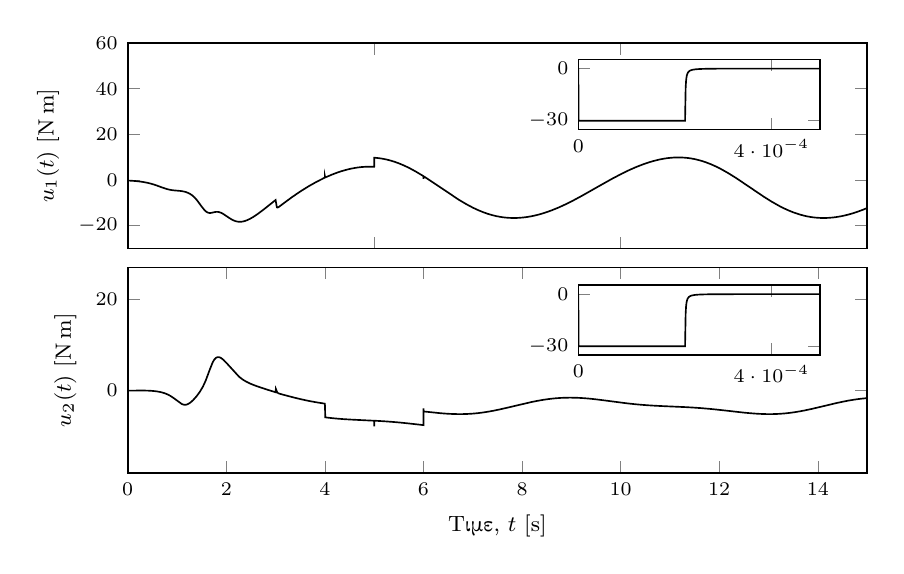
\begin{tikzpicture}

\begin{axis}[%
width=0.968\figurewidth,
height=0.478\figureheight,
at={(0\figurewidth,0.522\figureheight)},
scale only axis,
xmin=0,
xmax=15,
xtick={0,5,10,15},
xticklabels={\empty},
ymin=-30,
ymax=60,
ylabel style={font=\color{white!15!black}},
ylabel={$u_1(t)$ [\si{\newton\metre}]},
axis background/.style={fill=white},
xlabel style={font=\footnotesize},ylabel style={font=\footnotesize},ticklabel style={font=\scriptsize},x tick label style={font=\scriptsize},y tick label style={font=\scriptsize},legend style={font=\scriptsize}
]
\addplot [color=black, forget plot]
  table[row sep=crcr]{%
0	-0\\
0.00022104904765996	-30\\
0.000442188616226247	-0.211453145612346\\
0.0660909396420379	-0.287445637667702\\
0.125004559562441	-0.376158535062046\\
0.180836592403185	-0.482488929225077\\
0.238352962637364	-0.619646064447686\\
0.295869332871543	-0.790515174027806\\
0.353667900028302	-1.00249984223026\\
0.415275832280877	-1.28011420695399\\
0.482491988331201	-1.6511433410095\\
0.563810102574866	-2.19748341517072\\
0.6844645913154	-3.14329775097707\\
0.781646951374317	-3.86039400797483\\
0.83978726623678	-4.18815198481265\\
0.884145040684103	-4.37080073299842\\
0.928879084281661	-4.50076868679362\\
0.974273416120834	-4.59345523676731\\
1.06080859008615	-4.75362394617368\\
1.09718153438933	-4.85355496053767\\
1.1335544786925	-4.9944113357354\\
1.17005161525565	-5.19122887641064\\
1.21400059720344	-5.52266634511755\\
1.25762669710135	-5.9791086454462\\
1.30536957908527	-6.65834360250129\\
1.35375535842587	-7.57447250826529\\
1.40564304291874	-8.83309430413215\\
1.48976431658434	-11.3177351238887\\
1.56046829556299	-13.2482952831889\\
1.60146599775031	-13.9969483752658\\
1.62916137848991	-14.2929849599764\\
1.64762496564964	-14.3963464727832\\
1.66770998405894	-14.4319970194063\\
1.67668430401458	-14.4255615165481\\
1.69311477392242	-14.3849088088867\\
1.7229393737312	-14.2482280955827\\
1.77398139498391	-13.9983873007427\\
1.79727678590701	-13.9401419239149\\
1.8128070465224	-13.9325184257039\\
1.8287890932211	-13.9535470471163\\
1.8452229260031	-14.00667164927\\
1.86987367517611	-14.1454289380203\\
1.89843663060344	-14.3884739350057\\
1.93912870867609	-14.8604352593499\\
2.01043366822288	-15.8932457988521\\
2.10035732748982	-17.1699170700329\\
2.14946381145791	-17.7059442015112\\
2.18629367443398	-18.0005441756846\\
2.22312353741005	-18.1946635192111\\
2.24767677939409	-18.267129663822\\
2.27316500464543	-18.2946638650086\\
2.29312237029278	-18.2831614901283\\
2.31502381638358	-18.2383444701262\\
2.34110293511899	-18.1431725654307\\
2.3777522325733	-17.9383269209141\\
2.42028713577528	-17.6077992359425\\
2.47911254338534	-17.0129542909185\\
2.54775809132914	-16.1597582280249\\
2.63890581543842	-14.8359960587708\\
2.76601452048722	-12.7649115299107\\
3.00000642988953	-8.74271156731254\\
3.02536547326779	-11.9146197219756\\
3.03799463503343	-12.0561538324985\\
3.04763366127573	-12.0105222530946\\
3.06566684334104	-11.7858889846949\\
3.14076315203248	-10.5513056501756\\
3.33460493739823	-7.45704723171126\\
3.51806552154855	-4.76769827052386\\
3.67683292291718	-2.64363566924462\\
3.8288099641662	-0.798035956158248\\
3.95699861699376	0.607949132170969\\
4.0000560688419	1.12077570770816\\
4.00051820005105	1.69527506638823\\
4.00609575995756	1.11578798137667\\
4.01504180132752	1.1928162707408\\
4.13458434016859	2.31027849199505\\
4.23761499153439	3.16352389944021\\
4.34436144777517	3.93477417228232\\
4.43984349486218	4.52259639249391\\
4.52459661680067	4.95982549955039\\
4.6073232816453	5.30661933690248\\
4.67671279888257	5.53427575235917\\
4.74028240104325	5.69055278756812\\
4.78997409975648	5.77699142553015\\
4.82502334695534	5.81873593826496\\
4.8619940422109	5.84527536161605\\
4.89896473746647	5.85362868941011\\
4.93995242044692	5.84137214877086\\
4.98495709115226	5.80154534991976\\
5.00000035233748	5.78202481124013\\
5.00266773753172	9.78075416458626\\
5.04061420208204	9.71658636848957\\
5.08369246107973	9.61897651384106\\
5.13319634173576	9.4746388346283\\
5.1950596486038	9.24565865507477\\
5.26715627071125	8.91052477811907\\
5.3392528928187	8.50215173433269\\
5.4164973684884	7.98425798264662\\
5.49631577093924	7.36357984803871\\
5.60327750835441	6.40056776862869\\
5.71185084821177	5.27849281986934\\
5.83692468321024	3.82292451821327\\
5.98888235353401	1.856312373628\\
6.00002283879784	1.61220595976411\\
6.00010310518725	0.552082126790452\\
6.00022886960313	1.51857257745763\\
6.00029682093976	1.43074944268944\\
6.00044036232342	1.6401148628349\\
6.00065715924	1.68008771052139\\
6.0008568249131	1.68956371295983\\
6.01011780849129	1.56749736927722\\
6.19763768005213	-1.09795862781075\\
6.71662496067965	-8.61625575684744\\
6.86566708427418	-10.530049361102\\
7.00608095719842	-12.1394830744799\\
7.11924838037918	-13.2763532967996\\
7.23241580355994	-14.256100922391\\
7.30786075234712	-14.8175303648728\\
7.39896695805906	-15.3949365498037\\
7.4772218897987	-15.8019986729719\\
7.55815572326211	-16.1363575656193\\
7.62488362723816	-16.3460983460102\\
7.66936889655553	-16.4531109347159\\
7.7276777010745	-16.5540541480547\\
7.78598650559347	-16.6109528449828\\
7.81514090785296	-16.6231014534686\\
7.84429531011245	-16.6245077597216\\
7.87736636710396	-16.6132245568588\\
7.91043742409548	-16.5883961817216\\
7.96427275492981	-16.5194102755563\\
8.01810808576414	-16.4156352310731\\
8.07194341659847	-16.2777876642856\\
8.12985931338885	-16.0922901439331\\
8.18777521017923	-15.8691486574556\\
8.24569110696962	-15.6093217756476\\
8.333356538999	-15.1484319063835\\
8.42102197102838	-14.6092657071175\\
8.50868740305776	-13.995534949185\\
8.59951167465071	-13.2852820831616\\
8.74048634138547	-12.0441105694835\\
8.88146100812023	-10.6521356307547\\
9.02243567485499	-9.13257691786571\\
9.21409484346862	-6.90992521350821\\
9.53198374878137	-3.01311646339606\\
9.82222463020225	0.511590903219883\\
10.0332480116159	2.90327476308499\\
10.1756385548839	4.38643805252077\\
10.3199552802739	5.75468540816431\\
10.4681243699078	6.99484408894088\\
10.5669037629971	7.71765046630894\\
10.6670256159261	8.3573527666386\\
10.7684899286949	8.90308552034672\\
10.8699542414638	9.33844629600535\\
10.9206863978482	9.51253552593068\\
10.9714185542326	9.65642193149491\\
11.022150710617	9.76927911911727\\
11.0728828670014	9.85031308551369\\
11.1236150233858	9.89876999844512\\
11.1743471797702	9.91394462609226\\
11.2250793361546	9.89518930389501\\
11.2758114925391	9.84192332039274\\
11.3265436489235	9.75364259692671\\
11.3772758053079	9.62992952971173\\
11.4280079616923	9.47046285839028\\
11.4787401180767	9.27502742125156\\
11.5294722744611	9.04352365428329\\
11.6309365872299	8.4725449037877\\
11.7324008999988	7.75937292054799\\
11.8338652127676	6.90821612434279\\
11.9353295255364	5.92581817381802\\
12.0367938383052	4.82155148942\\
12.1889903074585	2.96359329081037\\
12.3418833995579	0.900177819007205\\
12.5990272962112	-2.83852830220068\\
12.907599972195	-7.34594893123457\\
13.061886310187	-9.43480805753326\\
13.2161726481789	-11.3265231602978\\
13.3190302068402	-12.4522852243365\\
13.4218877655015	-13.4556110204808\\
13.5247453241628	-14.3275927569089\\
13.6276028828241	-15.0621048229691\\
13.7312294426775	-15.6595086729378\\
13.7834272232003	-15.9057396114133\\
13.8356250037231	-16.1153405440477\\
13.8878227842459	-16.2884639901567\\
13.9400205647687	-16.4253638071579\\
13.9922183452915	-16.5263819327925\\
14.0444161258143	-16.5919355657747\\
14.0966139063371	-16.6225050629841\\
14.1488116868599	-16.618622802044\\
14.1918356619446	-16.5899268827789\\
14.2348596370294	-16.5385536672653\\
14.2778836121141	-16.4648548898559\\
14.3209075871988	-16.3691926813138\\
14.3639315622835	-16.2519377635176\\
14.449979512453	-15.954168692465\\
14.5373912922607	-15.5679940811031\\
14.6248030720684	-15.1008246791388\\
14.7122148518761	-14.5561686828619\\
14.8123187871912	-13.842025604449\\
14.9251148780139	-12.9288855368142\\
15	-12.2635891594649\\
};
\end{axis}

\begin{axis}[%
width=0.316\figurewidth,
height=0.163\figureheight,
at={(0.59\figurewidth,0.799\figureheight)},
scale only axis,
scaled x ticks = false,
xtick = {0, 4e-4},
ytick = {-30, 0},
xmin=0,
xmax=0.0005,
ymin=-35,
ymax=5,
axis background/.style={fill=white},
xlabel style={font=\footnotesize},ylabel style={font=\footnotesize},ticklabel style={font=\scriptsize},x tick label style={font=\scriptsize},y tick label style={font=\scriptsize},legend style={font=\scriptsize}
]
\addplot [color=black, forget plot]
  table[row sep=crcr]{%
0	-0\\
3.90358380286671e-07	-30\\
0.00022104904765996	-30\\
0.000222249302204602	-11.5368437967027\\
0.000223065415646317	-7.42752472699104\\
0.000223925092726063	-5.30007050854785\\
0.000224784769802255	-4.0738880026027\\
0.000225965946281548	-3.05904006589224\\
0.00022746862216394	-2.30036994363781\\
0.000228971298042779	-1.83190242914678\\
0.000230802659718421	-1.46106546368262\\
0.000232962707194417	-1.17571474622188\\
0.000235122754666861	-0.982158570051975\\
0.000237446240248573	-0.834100610763823\\
0.000239933163939554	-0.71856113424365\\
0.000242420087626982	-0.631824339021652\\
0.000244907011317963	-0.564613301436204\\
0.000247808137068262	-0.50340711496866\\
0.00025070926281856	-0.455401349179969\\
0.00025308970619875	-0.423286764548962\\
0.00025547014957894	-0.396234740088062\\
0.000257850592955577	-0.373240123613936\\
0.000260403595948588	-0.352230803707499\\
0.000263129158547315	-0.333196047722769\\
0.000265854721149594	-0.317024200020139\\
0.000268580283748321	-0.303207427995215\\
0.000271860529569068	-0.289144239756816\\
0.000275140775393368	-0.277378643908563\\
0.000278421021214115	-0.267491466342044\\
0.000281935098985997	-0.258610347872668\\
0.000285683008709015	-0.250737234980615\\
0.000289430918432032	-0.244214058311982\\
0.00029317882815505	-0.238796371098985\\
0.00029718363716924	-0.234008346776097\\
0.000301188446183431	-0.23006730099122\\
0.000305193255197622	-0.226819054562803\\
0.000309358895115963	-0.224041770747494\\
0.000313685365942007	-0.221686891165465\\
0.000318011836768051	-0.21977073498314\\
0.000322338307590542	-0.21821081729831\\
0.000324713156047096	-0.2174813871559\\
0.000327088004503651	-0.216829679301739\\
0.000329462852956652	-0.216247389711512\\
0.000331837701413207	-0.215727114813259\\
0.000334212549869761	-0.215262250836965\\
0.000336587398326316	-0.214846904666054\\
0.000338962246779317	-0.214475815475822\\
0.000341613811631447	-0.214108032613378\\
0.000344265376480024	-0.213783774620079\\
0.000346916941328601	-0.213497923669486\\
0.000349568506180731	-0.213245966574711\\
0.000352220071029308	-0.213023922523963\\
0.000354871635881437	-0.212828279245677\\
0.000357523200730014	-0.212655937352004\\
0.000360535928891181	-0.212484944268336\\
0.000363548657052348	-0.212336999455829\\
0.000366561385213515	-0.212209054396954\\
0.000369574113374682	-0.212098463985008\\
0.000372586841539402	-0.212002932995965\\
0.000375599569700569	-0.211920469267096\\
0.000378612297861736	-0.211849343573228\\
0.00038210356971291	-0.211779137360384\\
0.000385594841560533	-0.211720144040829\\
0.000389086113411707	-0.211670661117324\\
0.000392577385262882	-0.211629244414826\\
0.000396068657114057	-0.211594668915218\\
0.000399559928965232	-0.21156589504475\\
0.000403051200812854	-0.211542040576731\\
0.000407194134250943	-0.211519092868247\\
0.000411337067689033	-0.211500978740876\\
0.000415480001127122	-0.211486837492838\\
0.000419622934565211	-0.211475961664643\\
0.000423765867999748	-0.2114677698133\\
0.000427908801437837	-0.211461783582465\\
0.000432051734875927	-0.211457609393246\\
0.000437120175551087	-0.211454500042716\\
0.000442188616226247	-0.211453145612346\\
0.000447257056901407	-0.211453170267262\\
0.000452325497576567	-0.211454278782558\\
0.000457393938251727	-0.211456239327237\\
0.000462462378926887	-0.211458869343844\\
0.000467530819602047	-0.211462025014157\\
0.000473995544719941	-0.211466637382493\\
0.000480460269837835	-0.211471745324559\\
0.00049338972007007	-0.211482955994178\\
0.000506319170302305	-0.211494971094606\\
};
\end{axis}

\begin{axis}[%
width=0.968\figurewidth,
height=0.478\figureheight,
at={(0\figurewidth,0\figureheight)},
scale only axis,
unbounded coords=jump,
xmin=0,
xmax=15,
xlabel style={font=\color{white!15!black}},
xlabel={Time, $t$ [\si{\second}]},
ymin=-18,
ymax=27,
ylabel style={font=\color{white!15!black}},
ylabel={$u_2(t)$ [\si{\newton\metre}]},
axis background/.style={fill=white},
xlabel style={font=\footnotesize},ylabel style={font=\footnotesize},ticklabel style={font=\scriptsize},x tick label style={font=\scriptsize},y tick label style={font=\scriptsize},legend style={font=\scriptsize}
]
\addplot [color=black, forget plot]
  table[row sep=crcr]{%
0	-0\\
2.26144578618914e-08	30\\
2.78048339907855e-08	-22.5\\
nan	nan\\
0.000178559106064569	-22.5\\
0.000178566503141298	30\\
nan	nan\\
0.000179967590113961	29.7665287940332\\
0.000457393938251727	0.000189085207733086\\
0.307372606918381	0.0234422350185888\\
0.376815546583263	0.0109659855760746\\
0.442162294701006	-0.0163229201581885\\
0.495935219541266	-0.0541595303454869\\
0.550147295703709	-0.110516093327533\\
0.604798523188336	-0.190789029219939\\
0.659449750672962	-0.300972235435079\\
0.70716865885796	-0.42798138100526\\
0.752576793943081	-0.581895836475535\\
0.810717108805548	-0.836926349228399\\
0.869233692818248	-1.17245134967958\\
0.928879084281661	-1.60298274740788\\
1.09718153438933	-2.92921756543783\\
1.1335544786925	-3.06898899288539\\
1.15780310822795	-3.10209238560028\\
1.17005161525565	-3.09937237337019\\
1.18230012228336	-3.08355204751014\\
1.20427461325725	-3.02307058374187\\
1.23345256509581	-2.88301518409765\\
1.27489720505854	-2.58303912630428\\
1.3235586678382	-2.11314338184531\\
1.39401761254276	-1.2690865084363\\
1.46377019479865	-0.25095278167635\\
1.52666712302162	0.900960180231205\\
1.58300241059057	2.22273056228974\\
1.6587356641033	4.43134778854157\\
1.7229393737312	6.18247324528386\\
1.75676140099601	6.81059015009902\\
1.78951165559931	7.17831854557297\\
1.8128070465224	7.30885024195408\\
1.8287890932211	7.34432552430301\\
1.8370060096121	7.34742366924189\\
1.85343984239411	7.32606345665419\\
1.86987367517611	7.27203224107924\\
1.89843663060344	7.11310984802887\\
1.93912870867609	6.77600128817348\\
2.00022937439817	6.1082256825583\\
2.25995340038612	3.03731481476479\\
2.33547447175621	2.41409202627594\\
2.40327317449449	1.97220474478677\\
2.47911254338534	1.57146670635117\\
2.57380029821751	1.15464245791481\\
2.69405365229036	0.694801155480537\\
2.86768054914104	0.0907569973782074\\
3.00000184035483	-0.350371220836582\\
3.00567721208393	0.399433323001112\\
3.01008178831102	0.279672480808411\\
3.03295773032383	-0.381330557798695\\
3.05182105445522	-0.553267807229496\\
3.07860331733364	-0.664213624588879\\
3.1649516561788	-0.923697984541466\\
3.3835275545762	-1.54362212649212\\
3.54048851604394	-1.94676617469833\\
3.67683292291718	-2.25874754964905\\
3.80750418304128	-2.52044812025344\\
3.91424546831271	-2.70605658466303\\
4.00001901744172	-2.85498017294094\\
4.00807493578286	-5.85103917896761\\
4.05438468543641	-5.91503039256433\\
4.15852422704419	-6.04056052483925\\
4.27117540206059	-6.15371790125629\\
4.38196534140949	-6.24517601266089\\
4.51080883932656	-6.33192492270013\\
4.66283489543511	-6.4160374755712\\
5.00001027675444	-6.59512827417644\\
5.00014256262783	-7.81601960586669\\
5.00266773753172	-6.58768125618218\\
5.11773051501875	-6.65649051688161\\
5.2431240633421	-6.74369637704252\\
5.38989123433812	-6.86462844169758\\
5.52292190508951	-6.99261906087821\\
5.68470751324744	-7.16975533181503\\
5.9103465915928	-7.44376845120045\\
6.00000007852381	-7.55568126719696\\
6.00011503423429	-3.90506065163592\\
6.00021192430769	-5.11351547577276\\
6.00032024244119	-4.47416664901833\\
6.00041154231959	-4.66510388355269\\
6.00051920077512	-4.54912855264566\\
6.00061402083379	-4.57843355015142\\
6.00072218717598	-4.55693880008457\\
6.3495195929053	-4.94875407828784\\
6.45486227753386	-5.03618424836797\\
6.53386929100528	-5.08691763746037\\
6.62839928417087	-5.12795811371958\\
6.71662496067965	-5.14451150657822\\
6.77544207835217	-5.14285161189641\\
6.83758430968933	-5.12943911951443\\
6.89374985885902	-5.10665509240721\\
6.97799818261357	-5.0530260212851\\
7.04380343159201	-4.99473159733483\\
7.11924838037918	-4.910297511423\\
7.19469332916636	-4.80750922050037\\
7.30786075234712	-4.62077571753917\\
7.41853069099397	-4.40403029108763\\
7.53591308860343	-4.14320894522807\\
7.69852329881502	-3.74366010090506\\
8.18777521017923	-2.50422341310161\\
8.28952382298431	-2.28156175304556\\
8.42102197102838	-2.02930987607316\\
8.50868740305776	-1.88700833663016\\
8.59951167465071	-1.76369597140677\\
8.69349478580722	-1.6634441369536\\
8.78747789696373	-1.59194752051725\\
8.88146100812023	-1.5494942608018\\
8.97544411927674	-1.53570766455246\\
9.0703504670084	-1.54982825005196\\
9.16618005131521	-1.59094727550299\\
9.26200963562203	-1.65668721696175\\
9.35783921992884	-1.74411309664377\\
9.47393557249719	-1.87416813067736\\
9.64808010134972	-2.10467226187018\\
10.1281750404612	-2.78095666718925\\
10.2705655837292	-2.9498242491458\\
10.4187346733631	-3.09860282185106\\
10.5669037629971	-3.2194671829004\\
10.7177577723105	-3.31736728130205\\
10.8699542414638	-3.39733265797969\\
11.3265436489235	-3.61699208578747\\
11.4787401180767	-3.71291837653487\\
11.6309365872299	-3.83032289220785\\
11.7831330563832	-3.97104611263311\\
11.9353295255364	-4.1336370682444\\
12.138258151074	-4.37571131313374\\
12.4961697375499	-4.80966779482085\\
12.5990272962112	-4.91723886551135\\
12.7018848548724	-5.00898138155912\\
12.8047424135337	-5.08035393921326\\
12.907599972195	-5.12707239061035\\
12.9590287515257	-5.13997186043989\\
13.0104575308563	-5.14532928105589\\
13.061886310187	-5.14277882730409\\
13.1133150895176	-5.13201068368458\\
13.1647438688483	-5.11277654015817\\
13.2161726481789	-5.08489441185319\\
13.3190302068402	-5.00281318937504\\
13.4218877655015	-4.8857680835286\\
13.5247453241628	-4.73498126390275\\
13.6276028828241	-4.55288247036193\\
13.7312294426775	-4.34136713165988\\
13.8878227842459	-3.97886728598217\\
14.0966139063371	-3.44620967987712\\
14.3639315622835	-2.75899969241878\\
14.4936854023568	-2.45274900491014\\
14.6248030720684	-2.17650084254813\\
14.7559207417799	-1.94274872787792\\
14.8687168326026	-1.78106164130854\\
14.9706028980085	-1.66910306989781\\
15	-1.64303629134377\\
};
\end{axis}

\begin{axis}[%
width=0.316\figurewidth,
height=0.163\figureheight,
at={(0.59\figurewidth,0.274\figureheight)},
scale only axis,
xmin=0,
xmax=0.0005,
ymin=-35,
ymax=5,
scaled x ticks = false,
xtick = {0, 4e-4},
ytick = {-30, 0},
axis background/.style={fill=white},
xlabel style={font=\footnotesize},ylabel style={font=\footnotesize},ticklabel style={font=\scriptsize},x tick label style={font=\scriptsize},y tick label style={font=\scriptsize},legend style={font=\scriptsize}
]
\addplot [color=black, forget plot]
  table[row sep=crcr]{%
0	-0\\
3.90358380286671e-07	-30\\
0.00022104904765996	-30\\
0.000222249302204602	-11.5368437967027\\
0.000223065415646317	-7.42752472699104\\
0.000223925092726063	-5.30007050854785\\
0.000224784769802255	-4.0738880026027\\
0.000225965946281548	-3.05904006589224\\
0.00022746862216394	-2.30036994363781\\
0.000228971298042779	-1.83190242914678\\
0.000230802659718421	-1.46106546368262\\
0.000232962707194417	-1.17571474622188\\
0.000235122754666861	-0.982158570051975\\
0.000237446240248573	-0.834100610763823\\
0.000239933163939554	-0.71856113424365\\
0.000242420087626982	-0.631824339021652\\
0.000244907011317963	-0.564613301436204\\
0.000247808137068262	-0.50340711496866\\
0.00025070926281856	-0.455401349179969\\
0.00025308970619875	-0.423286764548962\\
0.00025547014957894	-0.396234740088062\\
0.000257850592955577	-0.373240123613936\\
0.000260403595948588	-0.352230803707499\\
0.000263129158547315	-0.333196047722769\\
0.000265854721149594	-0.317024200020139\\
0.000268580283748321	-0.303207427995215\\
0.000271860529569068	-0.289144239756816\\
0.000275140775393368	-0.277378643908563\\
0.000278421021214115	-0.267491466342044\\
0.000281935098985997	-0.258610347872668\\
0.000285683008709015	-0.250737234980615\\
0.000289430918432032	-0.244214058311982\\
0.00029317882815505	-0.238796371098985\\
0.00029718363716924	-0.234008346776097\\
0.000301188446183431	-0.23006730099122\\
0.000305193255197622	-0.226819054562803\\
0.000309358895115963	-0.224041770747494\\
0.000313685365942007	-0.221686891165465\\
0.000318011836768051	-0.21977073498314\\
0.000322338307590542	-0.21821081729831\\
0.000324713156047096	-0.2174813871559\\
0.000327088004503651	-0.216829679301739\\
0.000329462852956652	-0.216247389711512\\
0.000331837701413207	-0.215727114813259\\
0.000334212549869761	-0.215262250836965\\
0.000336587398326316	-0.214846904666054\\
0.000338962246779317	-0.214475815475822\\
0.000341613811631447	-0.214108032613378\\
0.000344265376480024	-0.213783774620079\\
0.000346916941328601	-0.213497923669486\\
0.000349568506180731	-0.213245966574711\\
0.000352220071029308	-0.213023922523963\\
0.000354871635881437	-0.212828279245677\\
0.000357523200730014	-0.212655937352004\\
0.000360535928891181	-0.212484944268336\\
0.000363548657052348	-0.212336999455829\\
0.000366561385213515	-0.212209054396954\\
0.000369574113374682	-0.212098463985008\\
0.000372586841539402	-0.212002932995965\\
0.000375599569700569	-0.211920469267096\\
0.000378612297861736	-0.211849343573228\\
0.00038210356971291	-0.211779137360384\\
0.000385594841560533	-0.211720144040829\\
0.000389086113411707	-0.211670661117324\\
0.000392577385262882	-0.211629244414826\\
0.000396068657114057	-0.211594668915218\\
0.000399559928965232	-0.21156589504475\\
0.000403051200812854	-0.211542040576731\\
0.000407194134250943	-0.211519092868247\\
0.000411337067689033	-0.211500978740876\\
0.000415480001127122	-0.211486837492838\\
0.000419622934565211	-0.211475961664643\\
0.000423765867999748	-0.2114677698133\\
0.000427908801437837	-0.211461783582465\\
0.000432051734875927	-0.211457609393246\\
0.000437120175551087	-0.211454500042716\\
0.000442188616226247	-0.211453145612346\\
0.000447257056901407	-0.211453170267262\\
0.000452325497576567	-0.211454278782558\\
0.000457393938251727	-0.211456239327237\\
0.000462462378926887	-0.211458869343844\\
0.000467530819602047	-0.211462025014157\\
0.000473995544719941	-0.211466637382493\\
0.000480460269837835	-0.211471745324559\\
0.00049338972007007	-0.211482955994178\\
0.000506319170302305	-0.211494971094606\\
};
\end{axis}
\end{tikzpicture}%
    \end{frame}
    
    \appendix
    
    \begin{frame}[plain,c]
        \begin{center}
            Ευχαριστώ για την προσοχή σας\\~\
            
            \pause
            \LARGE Ερωτήσεις?
        \end{center}
    \end{frame}

    \begin{frame}
        \frametitle{Ακολουθία ολοκληρωτών}
        Για ένα σύστημα με ομοιόμορφο σχετικό βαθμό $\qty{r_1, \ldots r_m}$, ορίζουμε ως ακολουθία ολοκληρωτών $(A,B,C)$ τους ακόλουθους πίνακες:
        \begin{align*}
            A &= \bdiag\pqty{A_1, \ldots, A_m}\\
            B &= \bdiag\pqty{B_1, \ldots, B_m}\\
            C &= \bdiag\pqty{C_1, \ldots, C_m}
        \end{align*}
        \[
            A_i = \begin{bmatrix}
                0 & 1 & \cdots & \cdots & 0 \\
                0 & 0 & 1 & \cdots & 0 \\
                \vdots & & & & \vdots \\
                0 & \cdots & \cdots & 0 & 1 \\
                0 & \cdots & \cdots & \cdots & 0
            \end{bmatrix}_{r_i \times r_i}\ 
            B_i = \bmqty{0\\ 0\\ \vdots\\ 0\\ 1}_{r_i \times 1}\ 
            C_i^\T = \begin{bmatrix}
                1 \\ 0 \\ \vdots \\ 0 \\ 0
            \end{bmatrix}_{r_i \times 1}
        \]
    \end{frame}
\end{document}